%10MB

\documentclass[10pt,finnish,a5paper]{scrartcl}

\usepackage[left=1.5cm,right=1.5cm,top=1.5cm,bottom=2cm]{geometry}
\usepackage{fontspec}
\usepackage{babel}
\usepackage{microtype}
\usepackage{multicol}
\usepackage{xcolor}
\usepackage{enumitem}
\usepackage{ragged2e}
\usepackage{graphicx}
\usepackage{wallpaper}
\usepackage{lipsum}
\usepackage[labelformat=empty]{caption}
\usepackage[export]{adjustbox}
\usepackage{calc}
\usepackage{pstricks}
\usepackage{contour}
\usepackage{multirow}
\usepackage{makecell}
\contourlength{2pt}

% \usepackage{draftwatermark}
% \SetWatermarkText{\textbf{LUONNOS}}
% \SetWatermarkScale{1}

\newenvironment{Figure}
  {\par\medskip\noindent\minipage{\linewidth}}
  {\endminipage\par\medskip}

\definecolor{link}{HTML}{f7941e}

\RedeclareSectionCommands[tocraggedentrytext]{section}

\setlength{\RaggedRightParindent}{\parindent}
\RaggedRight
\setmainfont[Ligatures=TeX]{Ubuntu}
\newfontfamily\monofont{Ubuntu Mono}
\definecolor{kuru}{HTML}{f7941e}
\setcounter{secnumdepth}{0}
\setcounter{tocdepth}{2}
\addto\captionsfinnish{\renewcommand{\contentsname}{Tässä numerossa}}
\addtokomafont{sectionentry}{\normalfont}
\addtokomafont{disposition}{\rmfamily\color{kuru}}
\addtokomafont{caption}{\footnotesize}
\setkomafont{subsection}{\normalfont\itshape}
\setenumerate{leftmargin=*}
\setitemize{leftmargin=*}
\frenchspacing
\def\UrlBreaks{\do\/\do-}

\usepackage[automark, autooneside=false]{scrlayer-scrpage}
\pagestyle{scrheadings}
\setkomafont{pageheadfoot}{}% not special font for page head and foot
% \clearpairofpagestyles
% \ihead{\leftmark}
% \ohead{\Ifstr{\leftmark}{\rightbotmark}{}{\rightbotmark}}
% \ohead{\Ifstr{\rightbotmark}{\leftmark}{}{\leftmark}}
\ihead{}
\chead{}
\ohead{\color{kuru}\rightmark}
% \ihead{\headmark}
% \markright{
% }
\cfoot{\pagemark}

% \newcommand{\dit}{\raisebox{0.47ex}{.}}
% \newcommand{\dah}{\raisebox{-0.0ex}{\textbf{-}}}
% \newcommand{\daaah}[1]{\raisebox{0.64ex}{\rule{#1}{2pt}}}

% \usepackage{listings}
% \newcommand{\morse}[1]{\
% 	\lstset{
% 		basicstyle=\Large,
% 		literate={A}{\dit\dah}3{B}{\dah\dit\dit\dit}3{C}{\dah\dit\dah\dit}4
% 			{D}{\dah\dit\dit}3{E}{\dit}2{F}{\dit\dit\dah\dit}3
% 			{G}{\dah\dah\dit}4{H}{\dit\dit\dit\dit}3{I}{\dit\dit}2
% 			{J}{\dit\dah\dah\dah}4{K}{\dah\dit\dah}3{L}{\dit\dah\dit\dit}3
% 			{M}{\dah\dah}3{N}{\dah\dit}2{O}{\dah\dah\dah}4
% 			{P}{\dit\dah\dah\dit}4{Q}{\dah\dah\dit\dah}4{R}{\dit\dah\dit}3
% 			{S}{\dit\dit\dit}3{T}{\dah}2{U}{\dit\dit\dah}3
% 			{V}{\dit\dit\dit\dah}3{W}{\dit\dah\dah}4{X}{\dah\dit\dit\dah}3
% 			{Y}{\dah\dit\dah\dah}4{Z}{\dah\dah\dit\dit}3{Å}{\dit\dah\dah\dit\dah}5
% 			{Ä}{\dit\dah\dit\dah}4{Ö}{\dah\dah\dah\dit}4{0}{\dah\dah\dah\dah\dah}5
% 			{1}{\dit\dah\dah\dah\dah}5{2}{\dit\dit\dah\dah\dah}5{3}{\dit\dit\dit\dah\dah}5
% 			{4}{\dit\dit\dit\dit\dah}4{5}{\dit\dit\dit\dit\dit}4{6}{\dah\dit\dit\dit\dit}4
% 			{7}{\dah\dah\dit\dit\dit}5{8}{\dah\dah\dah\dit\dit}5{9}{\dah\dah\dah\dah\dit}5
% 			{?}{\dit\dit\dah\dah\dit\dit}5{/}{\dah\dit\dit\dah\dit}5{=}{\dah\dit\dit\dit\dah}4
% 			{:}{\dah\dah\dah\dit\dit\dit}5{,}{\dah\dah\dit\dit\dah\dah}5{.}{\dit\dah\dit\dah\dit\dah}5
% 			% {}{}4{}{}4{}{}4
% 	}
% 	\lstinline{#1}
% }
% \newcommand{\morseprosign}[1]{\
% 	\lstset{
% 		basicstyle=\Large,
% 		literate={A}{\dit\dah}1{B}{\dah\dit\dit\dit}1{C}{\dah\dit\dah\dit}1
% 			{D}{\dah\dit\dit}1{E}{\dit}1{F}{\dit\dit\dah\dit}1
% 			{G}{\dah\dah\dit}1{H}{\dit\dit\dit\dit}1{I}{\dit\dit}1
% 			{J}{\dit\dah\dah\dah}1{K}{\dah\dit\dah}1{L}{\dit\dah\dit\dit}1
% 			{M}{\dah\dah}1{N}{\dah\dit}1{O}{\dah\dah\dah}1
% 			{P}{\dit\dah\dah\dit}1{Q}{\dah\dah\dit\dah}1{R}{\dit\dah\dit}1
% 			{S}{\dit\dit\dit}1{T}{\dah}1{U}{\dit\dit\dah}1
% 			{V}{\dit\dit\dit\dah}1{W}{\dit\dah\dah}1{X}{\dah\dit\dit\dah}1
% 			{Y}{\dah\dit\dah\dah}1{Z}{\dah\dah\dit\dit}1{Å}{\dit\dah\dah\dit\dah}1
% 			{Ä}{\dit\dah\dit\dah}1{Ö}{\dah\dah\dah\dit}1{0}{\dah\dah\dah\dah\dah}1
% 			{1}{\dit\dah\dah\dah\dah}1{2}{\dit\dit\dah\dah\dah}1{3}{\dit\dit\dit\dah\dah}1
% 			{4}{\dit\dit\dit\dit\dah}1{5}{\dit\dit\dit\dit\dit}1{6}{\dah\dit\dit\dit\dit}1
% 			{7}{\dah\dah\dit\dit\dit}1{8}{\dah\dah\dah\dit\dit}1{9}{\dah\dah\dah\dah\dit}1
% 			{?}{\dit\dit\dah\dah\dit\dit}1{/}{\dah\dit\dit\dah\dit}1{=}{\dah\dah\dah\dit\dit\dit}1
% 			{:}{\dah\dah\dah\dit\dit\dit}1{,}{\dah\dah\dit\dit\dah\dah}1{.}{\dit\dah\dit\dah\dit\dah}1
% 			% {}{}4{}{}4{}{}4
% 	}
% 	\lstinline{#1}
% }

% Packages needed:
\usepackage{tikz}
\usepackage[most]{tcolorbox}
\newtcolorbox{kuruboxtitle}[1][]{%
    enhanced,
    before skip=0mm,after skip=0mm, 
    width=1\textwidth, boxrule=0mm,
    colback=kuru, colframe=kuru, % Colors
    sharp corners,
    underlay={%
	    \fill[kuru] ([xshift=-10mm,yshift=2mm]frame.north west) -- ([xshift=8mm]frame.north east)
	    -- ([xshift=10mm,yshift=-2mm]frame.south east) -- ([xshift=-8mm]frame.south west)
	    -- cycle;
	    \fill[white] ([xshift=-6mm,yshift=-2mm]frame.north west) ellipse (1mm and 2mm);
	    \fill[white] ([xshift=-3mm,yshift=-2mm]frame.north west) ellipse (1mm and 2mm);
	    \fill[white] ([xshift=-4.5mm,yshift=-6mm]frame.north west) circle (1mm);
	    \fill[white] ([xshift=-4.5mm,yshift=-9mm]frame.north west) circle (1mm);
        },
    % drop fuzzy shadow, % Shadow
    title={#1},
}

\usepackage{titlesec}
\titleformat
{\section} % command
[display] % shape
{\bfseries\Large} % format
{\thechapter} % label
{0.5ex} % sep
{
	\clearpage
	\thispagestyle{plain}
	\begin{center}
		\begin{kuruboxtitle}[]
			\color{white}
} % before-code
[
		\end{kuruboxtitle}
	\end{center}
] % after-code

\titleformat
{\subsection} % command
[display] % shape
{\bfseries\large} % format
{\thechapter} % label
{0.32cm} % sep
{
} % before-code
[
] % after-code

\titleformat
{\subsubsection} % command
[display] % shape
{\bfseries} % format
{\thechapter} % label
{0.16cm} % sep
{
} % before-code
[
] % after-code

\usepackage[colorlinks,linkcolor=black,urlcolor=link]{hyperref}
\renewcommand{\theHsection}{\thepart.section.\thesection}
\urlstyle{same}

\begin{document}
\thispagestyle{empty}
\newgeometry{left=2cm,bottom=0cm}

\ThisCenterWallPaper{1.08}{assets/no_auto_compression/kansikuva}

% \vspace*{1.28cm}
\vspace*{11cm}

\newtcolorbox{logowhitebox}[1][]{%
    enhanced,
    before skip=0mm,after skip=0mm, 
    width=0.67\textwidth, boxrule=0mm,
    colback=kuru, colframe=kuru, % Colors
    sharp corners,
    underlay={%
	    \fill[white] ([xshift=-2mm,yshift=3mm]frame.north west) -- ([yshift=1mm]frame.north east)
	    -- ([xshift=1mm,yshift=-3mm]frame.south east) -- ([xshift=-1mm,yshift=-1mm]frame.south west)
	    -- cycle;
        },
    % drop fuzzy shadow, % Shadow
    title={#1},
}

\begin{logowhitebox}[]
	
\includegraphics[width=6cm]{assets/no_auto_compression/logo}
\end{logowhitebox}

\vspace*{1.28cm}

\newtcolorbox{kuruboxfrontpage}[1][]{%
    enhanced,
    before skip=0mm,after skip=0mm, 
    width=0.7\textwidth, boxrule=0mm,
    colback=kuru, colframe=kuru, % Colors
    sharp corners,
    underlay={%
	    \fill[kuru] ([xshift=-8mm,yshift=3mm]frame.north west) -- ([yshift=1mm]frame.north east)
	    -- ([xshift=1mm,yshift=-3mm]frame.south east) -- ([xshift=-7mm,yshift=-1mm]frame.south west)
	    -- cycle;
	    \fill[white] ([xshift=-4mm,yshift=-1mm]frame.north west) ellipse (1mm and 2mm);
	    \fill[white] ([xshift=-1mm,yshift=-1mm]frame.north west) ellipse (1mm and 2mm);
	    \fill[white] ([xshift=-2.5mm,yshift=-5mm]frame.north west) circle (1mm);
	    \fill[white] ([xshift=-2.5mm,yshift=-8mm]frame.north west) circle (1mm);
        },
    % drop fuzzy shadow, % Shadow
    title={#1},
}
\begin{kuruboxfrontpage}[]
	\color{white}{\large\bfseries 1/2025 Kurkisuon Rusakot ry}
\end{kuruboxfrontpage}

\clearpage
\restoregeometry
\thispagestyle{plain}

\ThisULCornerWallPaper{1}{assets/no_auto_compression/sisäkansikuva.jpg}

{\color{white}
\noindent \textbf{Tassu 1/2025} \\
\noindent ISSN 2984-5556}

\vfill

% \begin{multicols}{2}
\noindent\textbf{Päätoimittaja:}

Tanguy

\href{mailto:tanguy@gerome.fi}{tanguy@gerome.fi}

\medskip

\noindent\textbf{Muu toimitus:}

Janne

Vene

Pomppupallot

Päärynähyttyset

\medskip

\noindent\textbf{Julkaisija:}

Kurkisuon Rusakot ry, Helsinki

\medskip

\noindent Tarkista lippukunnan ajankohtaiset yhteystiedot nettisivuilta:

\href{https://kurkisuonrusakot.wordpress.com/}{kurkisuonrusakot.wordpress.com}

\medskip

\noindent Etu-, sisä- ja takakannen kuvat:

Tanguy

% \columnbreak
\vspace{-0.64cm}

\tableofcontents
% \end{multicols}

%STANDARD COLUMNS  
\section{Lippukunnanjohtajan tervehdys}

\begin{multicols}{2}
\noindent Haarapääskyt, räystäspääskyt ja tervapääskyt ovat jo aikaa sitten
saapuneet, merihanhilla on jo poikasia ja kuuluipa pellon laidalta
tuttu harmaasiepon ''tsri tsri tsri''. Kevät on jo täällä ja kesä on
aivan kulman takana. Valkovuokko, rentukka ja kirsikka ovat täydessä
kukassa ja ensimmäiset satakielet virittävät lauluaan aamuhämärässä.
Aivan, kesällä järjestetään lippukunnan \textit{Satakieli}"-kesäleiri!
Leirin lisäksi kesän toimintaan lukeutuvat \textit{Variksen vavahdus}
"=vaellus ja \textit{Piisaminhäntä}"-melonta. Olethan sinäkin mukana
kesän partiotapahtumissa?

Alkuvuoteen on jälleen mahtunut monenlaista partiotekemistä kuten
laskiaisriehaa, minihaikkia, partioparaatia ja lippukuntaretkeä. Olen
haltioissani siitä, kuinka paljon erilaista toimintaa pieni
lippukuntamme on pystynyt järjestämään; kevään toimintamme on
kartuttanut käyntikertoja yli seitsemänsataa! Tämä ei ole mikään
itsestäänselvyys, vaan mielekäs toiminta vaatii aina vapaaehtoisia,
tekijöitä ja johtajia -- unohtamatta itse osallistujia, joita ilman
tekeminen menettää merkityksensä.  

Osin partiotoiminnan mahdollistaa se, että lippukuntamme on
rekisteröity yhdistys. Sillä on vuosikokouksen valitsema hallitus, joka
vastaa toimintasuunnitelman toteutumisesta, päättää kalusto- ja muista
hankinnoista, ylläpitää jäsenrekisteriä, anoo avustuksia, edustaa
lippukuntaa piirin aluetapaamisissa\ldots\ Lippukunnan hallinto on
yleistäen kuin valtion, kunnan tai jonkin yrityksen hallinto
pienoiskoossa, joten partiotoiminnan tähän välillä tylsältäkin
vaikuttavaan osaan tutustuminen tarjoaa johtajalle paljon hyödyllisiä
tietoja ja taitoja, joista on aikuisena hyötyä muuallakin. Haluaisitko
sinä tutustua lippukunnan hallituksen tehtäviin? Kysy lisää
allekirjoittaneelta!

Tässä Tassussa pääset palaamaan viime vuoden pikkujouluretkeen,
riihitystunnelmiin vuonna 2018 ja tänä keväänä sekä tarpojien
minihaikille. Seikkailijoiden sivuilla (s. \pageref{sec:seikkailijat})
on paljon hauskaa luettavaa ja tekemistä. Julkistetaanpa lehdessä myös
viime numeron kuvakilpailun voittaja. Ja jos et ole vielä aloittanut,
nyt on oikea hetki alkaa pohtia, kuinka oikea ja nurja silmukka oikein
tehtiinkään, ottaa neulepuikot esiin ja osallistua Tassun
neulesuunnittelukilpailuun -- lue lisää sivulta
\pageref{sec:neulekilpailu}!

{\smallskip\noindent\centering ***\par\smallskip}

Kevättä varjosti Kurkisuon Rusakoiden perustajajäsenen ja ensimmäisen
lippukunnanjohtajan, \mbox{Eddien} poisnukkuminen. ''Yritä jättää tämä
maailma vähän parempana kuin sen löysit,'' kehotti lordi Baden"-Powell,
partioliikkeen perustaja viimeisessä viestissään maailman
partiolaisille. Sama ilmaisu löytyy Suomen Partiolaisten
partioneuvoston hyväksymistä partion yhteiskunnallisen toiminnan
linjauksista. Nykyisenä lippukunnanjohtajana olen vahvasti sitä mieltä,
että Eddie otti kehotuksesta vaarin.

Partioterveisin ja Eddien muistoa kunnioittaen

\smallskip

\noindent\hfill Janne

\vspace*{12cm}

\columnbreak

\null\vfill

\noindent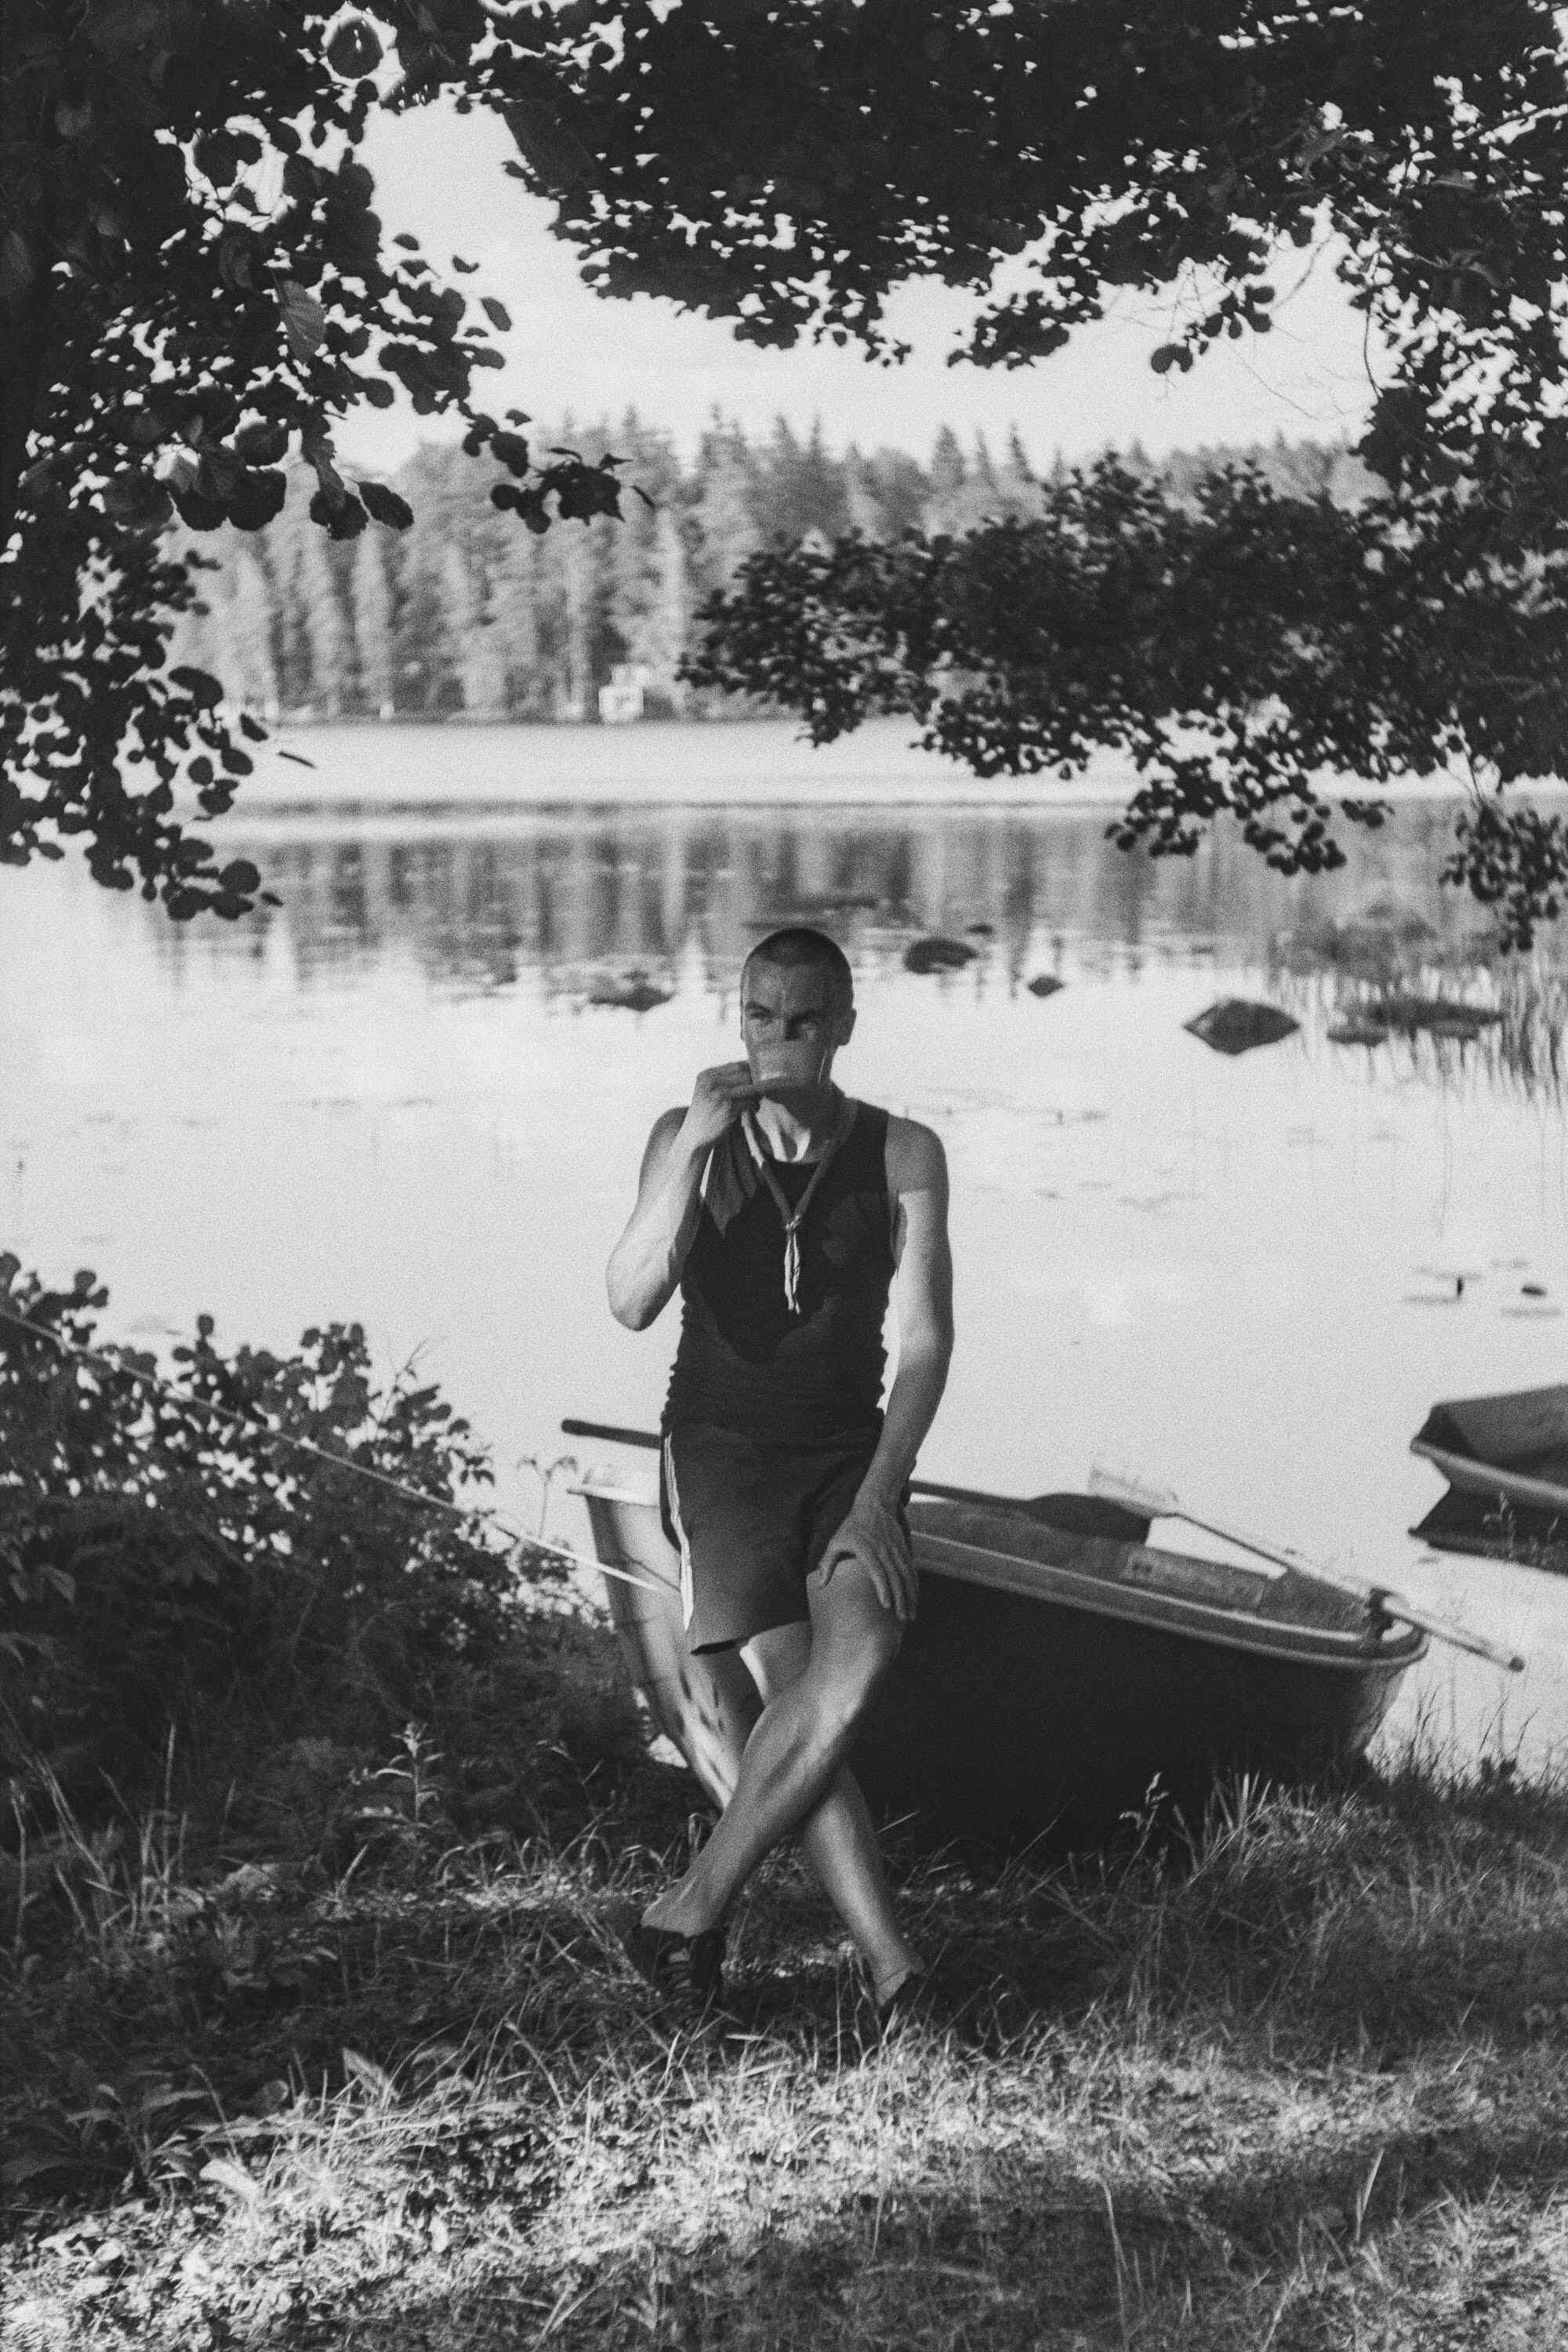
\includegraphics[width=\linewidth]{assets/lpkjohtajantervehdys} \\
{\small Lippukunnanjohtaja nauttimassa iltateestä \textit{Uikun uinti}
"=vaelluksen helteisen, kolmannen päivän päätteeksi Ruokojärven rannalla.\par}

\bigskip

\noindent\null\hfill Kuva: Tanguy
\end{multicols}


\section{Tassu ennen vanhaan}
\textit{Tassu on ilmestynyt säännöllisen epäsäännöllisesti lippukunnan perustamisvuodesta 1986
lähtien. Tällä palstalla muistellaan menneitä ja julkaistaan valittuja paloja takavuosien
lehdistä.}

% \textit{Päätoimittaja sai paketin, jossa on vuosikymmeniä Tassun painoksia ja
% yrittää digitalisoida ne lähiaikoina!}

\vspace*{0.32cm}
% \noindent Tällä kertaa mennään ajassa 20 vuotta taaksepäin, ja katsotaan mitä
% \mbox{KuRu:n} kolkat puuhasivat heidän syysretkellään vuonna 2004:

\newtcolorbox{StickyNote}[1][]{%
    enhanced,
    before skip=2mm,after skip=2mm, 
    width=\textwidth, boxrule=0.2mm, % width of the sticky note
    colback=kuru!50!white, colframe=kuru, % Colors
    attach boxed title to top right={xshift=0cm,yshift*=0mm-\tcboxedtitleheight},
    varwidth boxed title*=-3cm,
    % The titlebox:
    boxed title style={frame code={%
        \path[left color=kuru,right color=kuru,
        middle color=kuru]
        ([xshift=-0mm]frame.north west) -- ([xshift=0mm]frame.north east)
        [rounded corners=0mm]-- ([xshift=0mm,yshift=0mm]frame.north east)
        -- (frame.south east) -- (frame.south west)
        -- ([xshift=0mm,yshift=0mm]frame.north west)
        [sharp corners]-- cycle;
        },interior engine=empty,
    },
    sharp corners,rounded corners=southeast,arc is angular,arc=3mm,
    % The "folded paper" in the bottom right corner:
    underlay={%
        \path[fill=kuru!80!black] ([yshift=3mm]interior.south east)--++(-0.4,-0.1)--++(0.1,-0.2);
        \path[draw=kuru,shorten <=-0.05mm,shorten >=-0.05mm,color=kuru] ([yshift=3mm]interior.south east)--++(-0.4,-0.1)--++(0.1,-0.2);
        },
    % drop fuzzy shadow, % Shadow
    % fonttitle=\bfseries, 
    title={#1}
}

\vspace*{0.64cm}
\begin{StickyNote}[Julkaistu alunperin Tassussa x/xxxx]
	\monofont

\end{StickyNote}


\section{Johtajarusakot}

\textit{Monipuolisen partiotoiminnan mahdollistavat aktiiviset johtajat. Myös
kaikille heille partio on harrastus. Moni viihtyy partiossa ekaluokkalaisesta
\mbox{aikuiseksi} asti, sillä kaiken ikäisille riittää uutta koettavaa. Tässä Tassun
juttusarjassa tutustumme tarkemmin KuRu:n johtajiin.}

\vspace*{0.32cm}
% \noindent Tällä kertaa mennään ajassa 20 vuotta taaksepäin, ja katsotaan mitä
% \mbox{KuRu:n} kolkat puuhasivat heidän syysretkellään vuonna 2004:

\newtcolorbox{FaktaLaatikko}[1][]{%
    enhanced,
    before skip=2mm,after skip=2mm, 
    width=\textwidth, boxrule=0.2mm, % width of the sticky note
    colback=white, colframe=kuru, % Colors
    attach boxed title to top right={xshift=0cm,yshift*=0mm-\tcboxedtitleheight},
    varwidth boxed title*=-3cm,
    % The titlebox:
    boxed title style={frame code={%
        \path[left color=kuru,right color=kuru,
        middle color=kuru]
        ([xshift=-0mm]frame.north west) -- ([xshift=0mm]frame.north east)
        [rounded corners=0mm]-- ([xshift=0mm,yshift=0mm]frame.north east)
        -- (frame.south east) -- (frame.south west)
        -- ([xshift=0mm,yshift=0mm]frame.north west)
        [sharp corners]-- cycle;
        },interior engine=empty,
    },
    sharp corners,rounded corners=southeast,arc is angular,arc=3mm,
    % The "folded paper" in the bottom right corner:
    underlay={%
        \path[fill=kuru!80!black] ([yshift=3mm]interior.south east)--++(-0.4,-0.1)--++(0.1,-0.2);
        \path[draw=kuru,shorten <=-0.05mm,shorten >=-0.05mm,color=kuru] ([yshift=3mm]interior.south east)--++(-0.4,-0.1)--++(0.1,-0.2);
        },
    % drop fuzzy shadow, % Shadow
    % fonttitle=\bfseries, 
    title={#1}
}

\noindent \textbf{\Large Esittelyssä Leo}

\begin{multicols}{2}

\subsection*{Partiossa}
Tänä vuonna tulee täyteen 10 vuotta partiossa! Aloitin tosiaan partion pienenä ekaluokkalaisena vuonna 2015.

\vspace*{0.16cm}
\noindent\textbf{Millaisia partiotehtäviä sinulla on juuri nyt?}\\
Tällä hetkellä johdan seikkailijavartiota ja toimin (ainakin nimellisesti) lippukunnan varainhankintavastaavana.

\vspace*{\fill}
\columnbreak
\subsection*{``Siviilissä''}
Siviilissä opiskelen lukiossa toista vuotta ja kesäisin satunnaisia töitä. Nyt pari kesää ollut leiriohjaajana!

\vspace*{0.16cm}
\noindent\textbf{Mitä muuta harrastat?}\\
Partion lisäks harrastan fiiliksestä riippuen kaikkea sekalaista taiteilua ja muuta sekoilua. Soitan bändissä kitaraa ja laulan, jonka lisäks teen kuvataidetta ja käsitöitä aina kun huvittaa. Tällä hetkellä oon innostunut geokätköilystä!

\end{multicols}

% \vspace*{0.32cm}
% \vspace*{-0.64cm}
\begin{FaktaLaatikko}[Leo]

\begin{multicols}{2}
\vspace*{-0.64cm}
\vspace*{-0.16cm}
\begin{itemize}
\item Oon 17-vuotias ja asun Vantaan Hiekkaharjussa
\item \textbf{Kuuntelen mieluiten}: Kuuntelen paljon kaikkea erilaista musaa, mut tällä hetkellä kuuntelen paljon folkia ja rockia
\item \textbf{Katson mieluiten}: Oon tosi huono kattomaan yhtään mitään mut mun lempisarja on ehdottomasti Criminal Minds!
\item \textbf{Lautasella mieluiten}: Jotain kotitekosta, mausteista kasvisruokaa!
\end{itemize}
\columnbreak

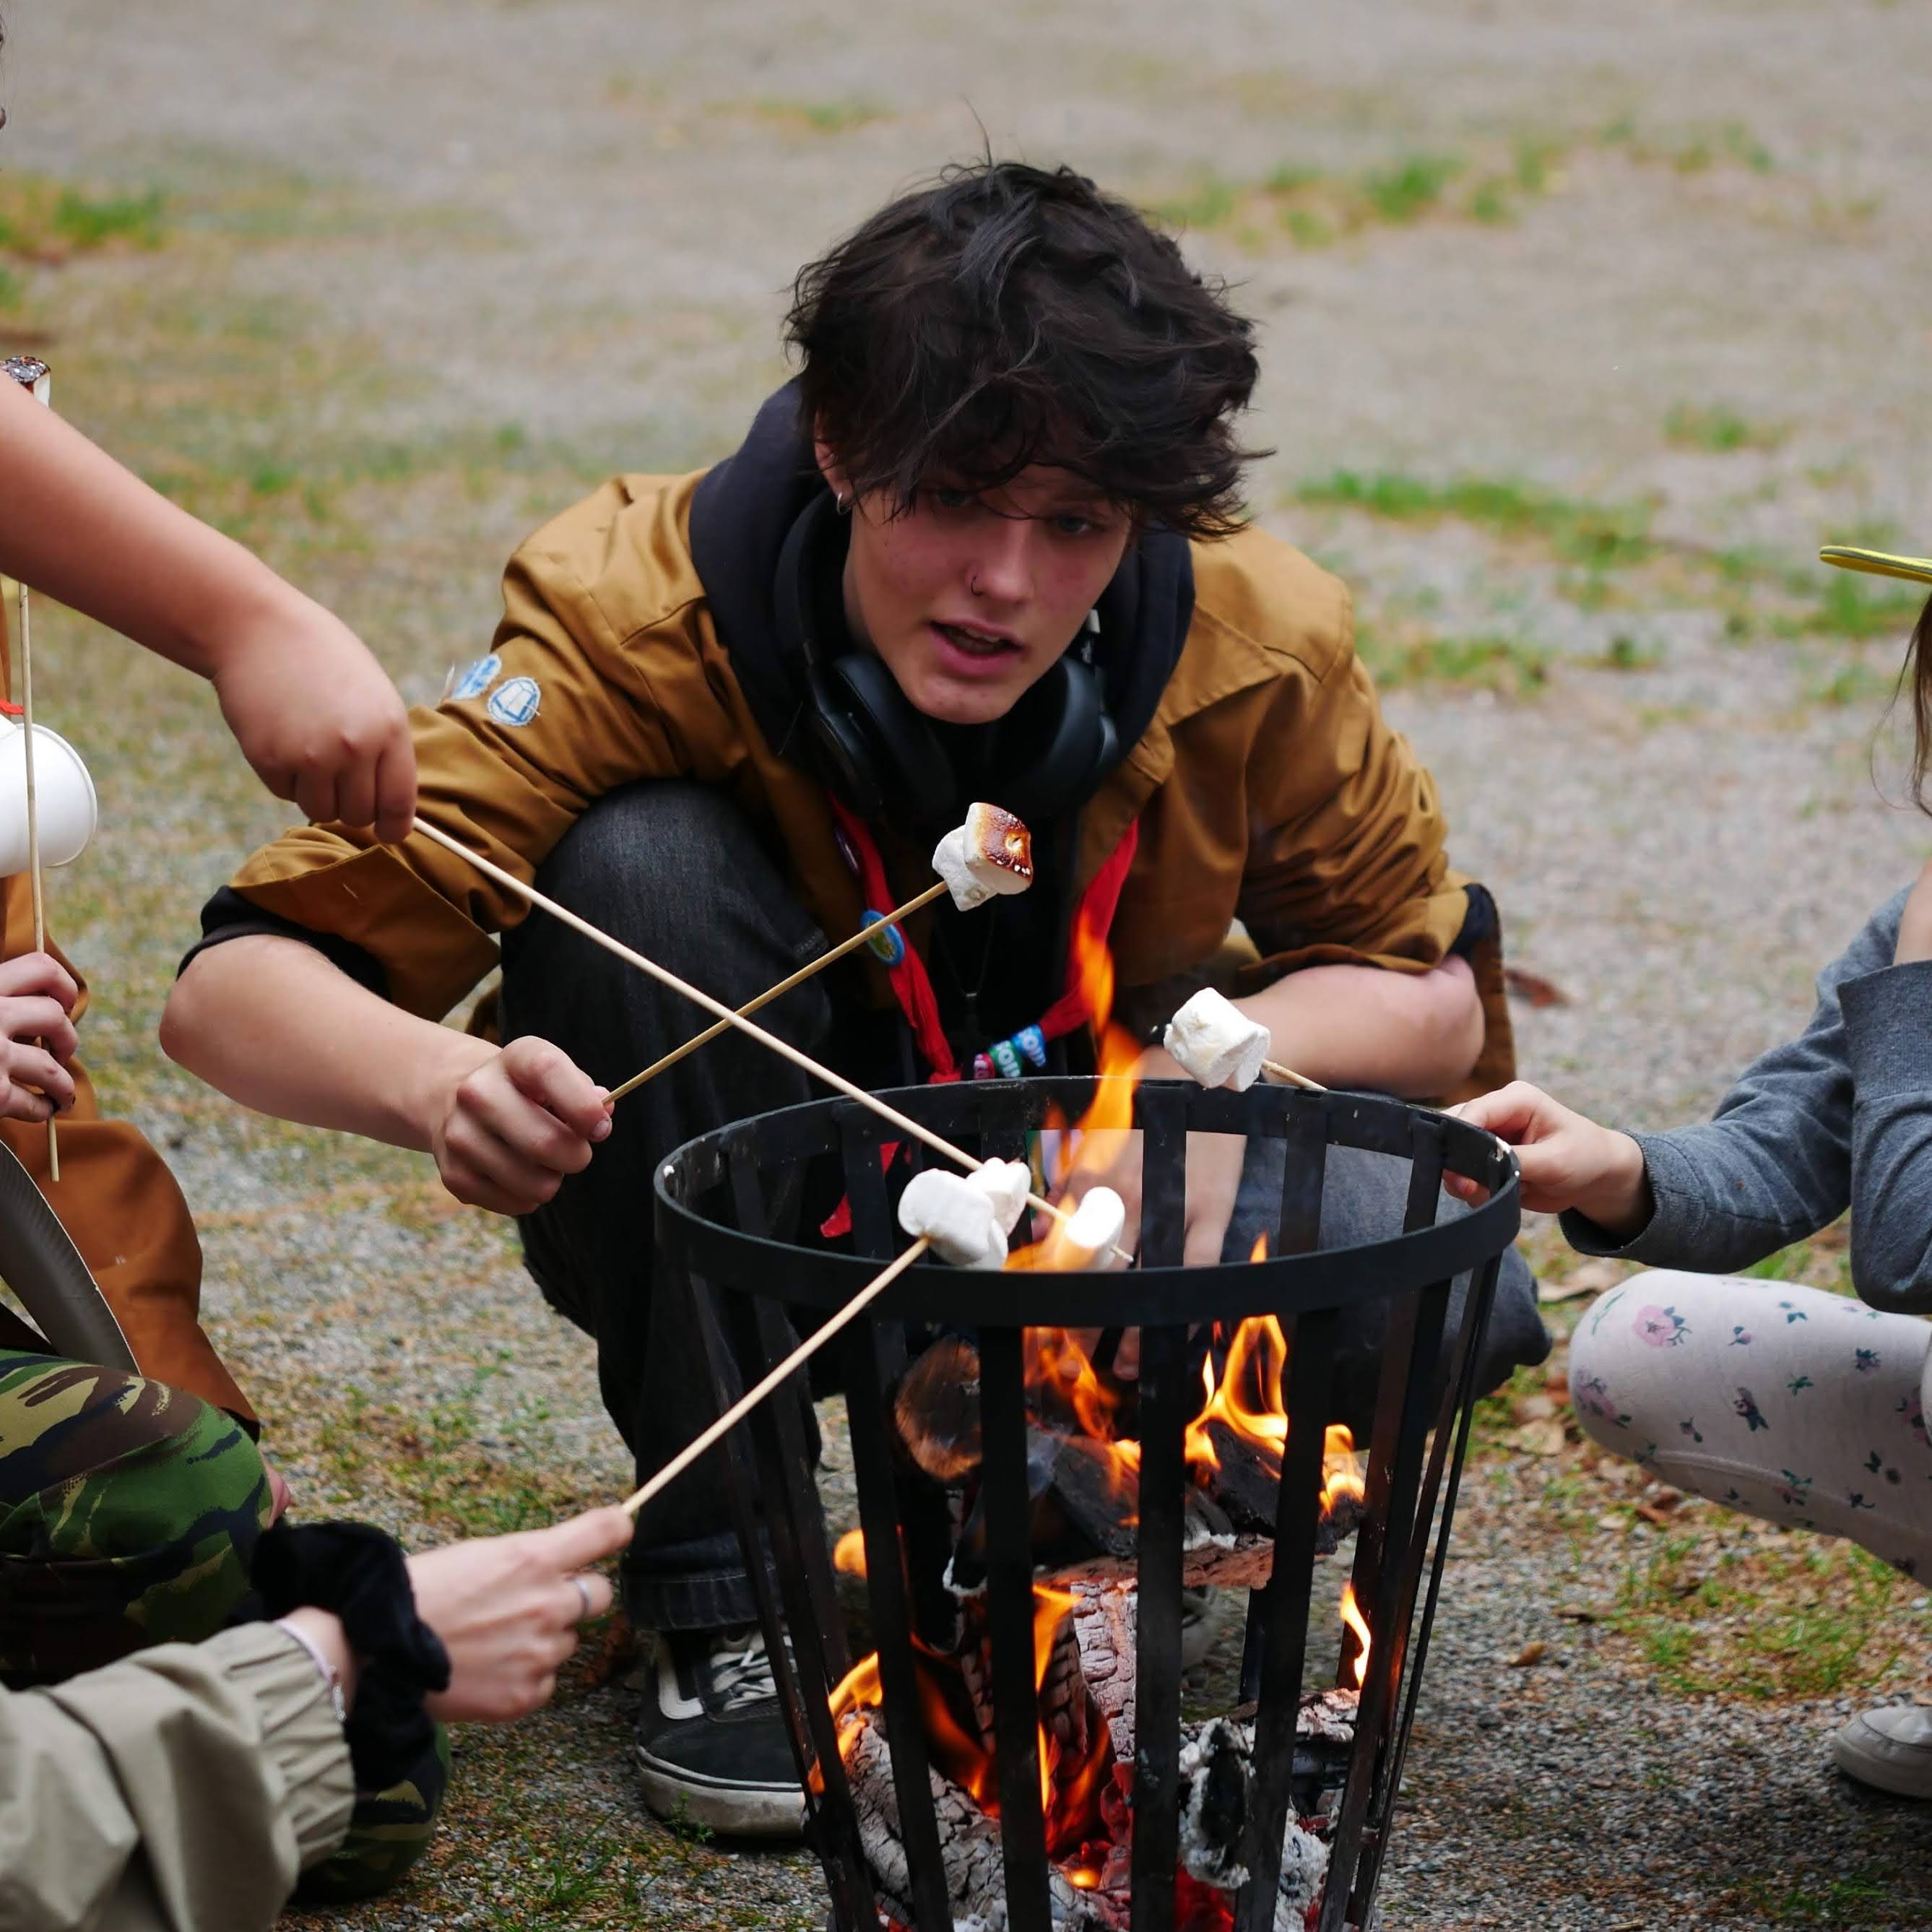
\includegraphics[width=1.02\columnwidth]{assets/johtajarusakot-leo.jpg}
\end{multicols}

\end{FaktaLaatikko}
\vspace*{-0.64cm}


%MISC COLUMNS
\section{Partionimi?}

\textit{Partionimi on partiotoiminnassa käytetty lempinimi. Aiemmin perinne 
käyttää partionimiä oli huomattavasti yleisempää, mutta nykyään vain 
harvalla lippukuntalaisella on partionimi. Ehkä tämä juttu innostaa sinut 
miettimään, haluasitko tulla kutsutuksi partionimellä ja elvyttää hiipuvaa 
perinnettä?}

\begin{multicols}{2}
\noindent Joissakin lippukunnissa partiolainen päättää partionimensä itse, 
joissakin lippukunnissa taas muut partiolaiset antavat sen hänelle. Voi olla 
esimerkiksi, että uusi jäsen ''kastetaan'' hänen ensimmäisellä 
leirillään leirikasteessa hänelle valitulla partionimellä. Partionimi voi 
olla myös henkilön oikea kutsumanimi, jona hän on tunnettu myös partion 
ulkopuolella.

Joskus partionimet saattavat säilyä partiolaisella läpi elämän. Joidenkin 
partionimissä voi mennä pidempään vakiintua ja nimi saattaa muuttaa 
kirjoitusasuaan tai vaihtua kokonaan hänen partiopolkunsa aikana. Oleellista 
on, että partionimi tarvitsee käyttöä jäädäkseen kanssapartiolaisten 
huulille.

Itse partionimi voi olla melkein mitä vain, mutta varsin tyypllistä on, että 
se liittyy jotkenkin partiolaisen luonteenpiirteisiin, etu- tai sukunimeen. Sen 
taustalla voi olla myös jokin hauska lausahdus tai tapahtuma; partionimi voi 
syntyä hyvin yllättävässäkin tilanteessa.

Tärkein tehtävä partionimellä on yksilöidä kantajansa. Joskus lisänimen 
käyttö voi tuntua keinotekoiselta, jos partiolaiset ovat tekemisissä 
toistensa kanssa myös harrastuksen ulkopuolella. Samaan aikaan partionimillä 
pystytään välttämään etunimikaimojen tuomat haasteet.

{\smallskip\noindent\centering ***\par\smallskip}

Kurkisuon Rusakoissa oli hyvin pitkään perinteenä, että kukin uusi kolkka 
ja vartiolainen keksi itselleen partionimen. Tyypillisesti nimi oli jokin 
eläin kuten Pupu, Koala, Delfiini, Leopardi tai Kyyhky, mutta myös muita 
luontoon liittyviä nimiä kuten Karvakuono, Salama, Pottu, Kaarna ja Ruusu 
esiintyi. Joskus nimi tuli jostain muusta yleisnimestä kuten Pamppu, Keiju, 
Stoori, Napero ja Pilkku, kun taas joskus se juontui jostain aivan muualta 
kuten Jepulski, Nici, Eevi, Luru ja Inni. 

Nykyään lippukunnan jäsenistä löytyy ainakin Jääkarhu, Kala, Kike, 
Kirsku, Käärme, Leijona, Nonna, Ristilukki ja Rusakko. Tiedätkö sinä, 
keitä he ovat?
\end{multicols}

\vfill

\noindent\null\hfill Teksti: Ristilukki

\section{Partiolaisuuden aakkoset}

\textit{Samoajavartio Vene listasi omat partiolaisuuden aakkosensa kevään 
2024 kokouksessaan. Kuinka hyvin nämä kuvaisivat juuri sinua?}

\begin{multicols}{3}
\setlength{\parindent}{0em}\setlength{\parskip}{.5em} {\large A}ina valmiina

{\large B}alansoitunut

{\large C}harmikas

{\large D}emokraattinen

{\large E}nerginen

{\large F}unktionaalinen

{\large G}uru

{\large H}ilpeä

{\large I}nnovatiivinen

{\large J}ohtaja

{\large K}ajahtanut

{\large L}uova

{\large M}onipuolinen

{\large N}ero

{\large O}ppivainen

{\large P}ystyvä

{\large Q}uadrifoglio

{\large R}eipas

{\large S}uvaitseva

{\large T}ietäväinen

{\large U}telias

{\large V}almis

{\large W}atti

{\large X}-treme leiriytyjä

{\large Y}ritteliäs

{\large Z}en

{\large Å}hå

{\large Ä}lykäs

{\large Ö}veri
\end{multicols}

\begin{figure}[!h]
\centering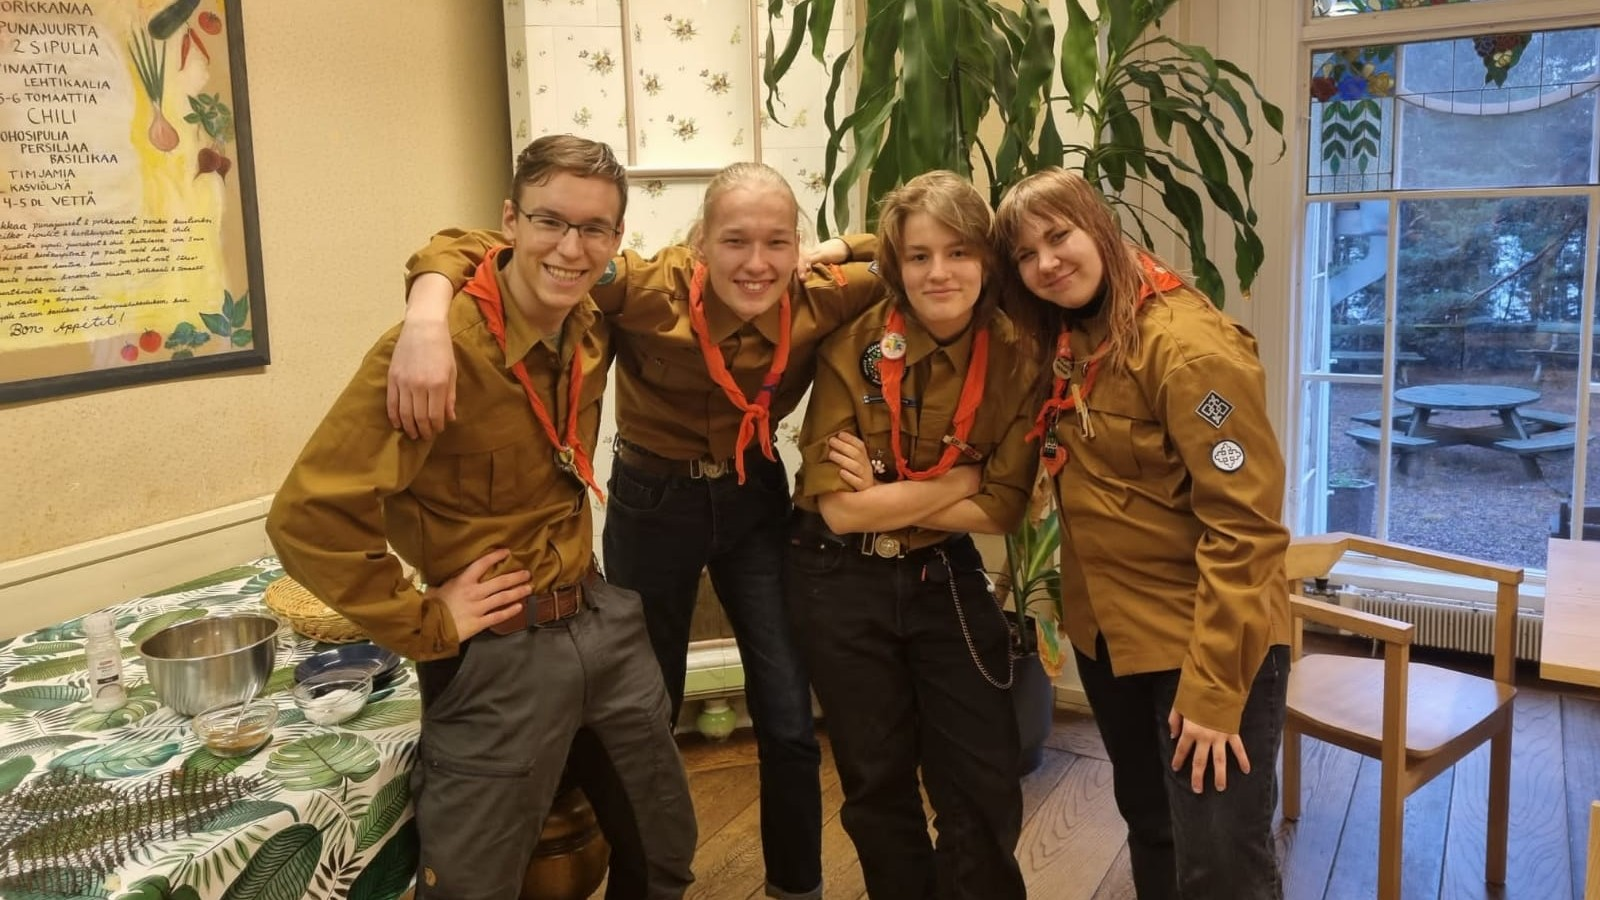
\includegraphics[width=\textwidth]{assets/vene}
\caption{\textit{Vene}-vartio.}
\end{figure}

\medskip

\noindent\null\hfill Kuva: ???


\section{Vene quotes}

\textit{Vene-vartion kokoukset ja retket ovat tunnetusti hyvin…no sanotaanko vaikka,
ettei Veneen tule koskaan tylsää. Koska meininki on hyvin nopeatempoista, Vene
sai kuningasidean alkaa dokumentoimaan yhdessä ollessa suusta päässeitä
lausahduksia, joita on noin vuoden keräämisen jälkeen jo satoja. Kuitenkin
suurin osa niistä sisältää ei-perheystävällistä kielenkäyttöä tai muuta
päivänvaloa kestämätöntä sisältöä, joten julkaisemaan päädyttiin vain hyvin
pieni osa sitaateista. Nämä lausahdukset ovat kerätty noin viimeisen puolen
vuoden ajalta.}

\vspace{0.64cm}
“Kahvi ON alkanut vaikuttaa” -Mikko

\smallskip
“Oikeesti mä alan velhoks” -Leo

\smallskip
“Täällä haiskahtaa mitoosi” -Elias

\smallskip
“Tää on mun työ teidän pitäis maksaa mulle!” -Janne

\smallskip
“Me ollaan samalla taajuudella tän ilmapallon kanssa” -Ahti

\smallskip
“Sori mä oon liian kermajuoma” -Mikael

\smallskip
“Any time Janne organizes something I expect it to be pure pain” -Tanguy

\smallskip
“Mummot on pahimpia!” -Mikko

\smallskip
“Mä just flippasin lautasellisen puuroo tohon lattialle…” -Leo

\smallskip
“Ruokamyrkytys-maxxing” -Elias

\smallskip
“Nyt on oikea hetki syrjäytyä” -Janne

\smallskip
“Kerranki sä ET oo ongelma” - Ahti

\smallskip
“Tää penkki on mua vastaan” -Mikael

\smallskip
“I think I got pranked by the weather forecast” -Tanguy



\section{Seikkailijoiden sivut}\label{sec:seikkailijat}


\vspace*{-0.32cm}
\begin{multicols}{2}
\noindent \textbf{Vitsi kulma!\\}
\bigskip
Mä meen ostaan Teslan\\
Tesla: ääh!\\
\bigskip
Voi vitsit! Täällä sataa lunta!\\
Lumi: Täh? En mä sada.

\vfill
\noindent Elna

\columnbreak
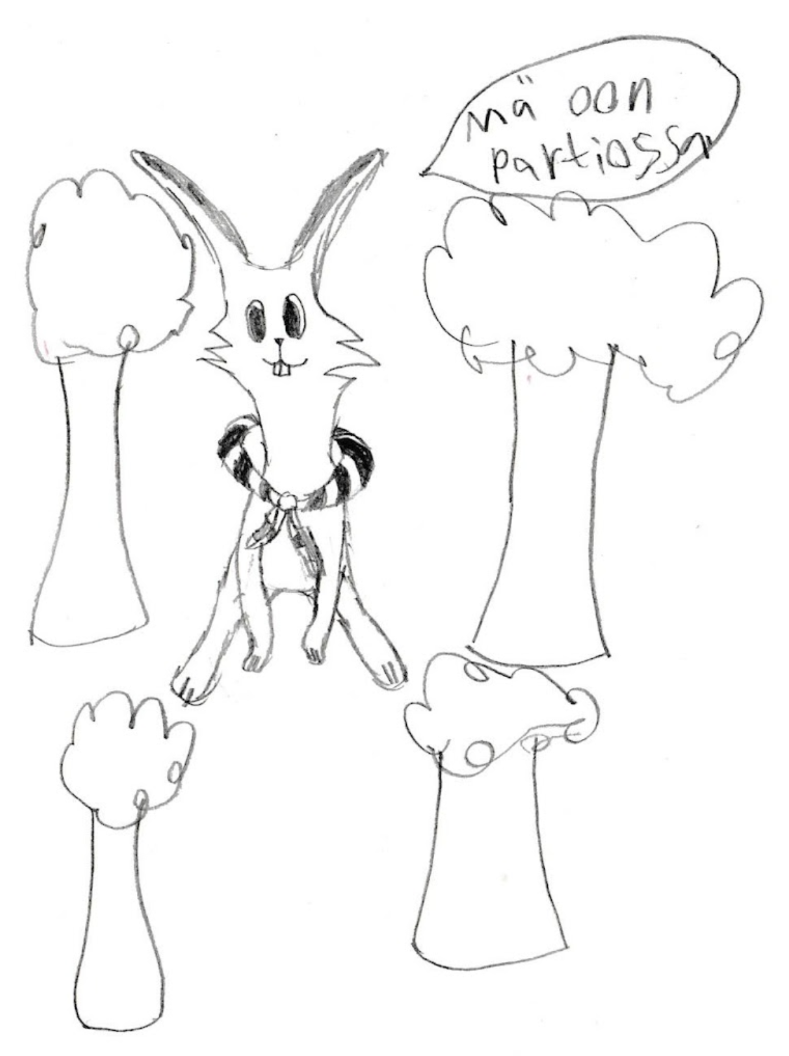
\includegraphics[width=0.42\textwidth]{assets/seikkailijat2}
\end{multicols}

\hrule

\begin{multicols}{2}
\noindent\textbf{Partion ristikko}
\begin{enumerate}
	\item Missä me ollaan
	\item Latinaksi se on Lepus Europaeus
	\item Puinen muki
	\item Kova ääni joka kuuluu ihmisistä
	\item Pelokkaan vastakohta
\end{enumerate}
\columnbreak
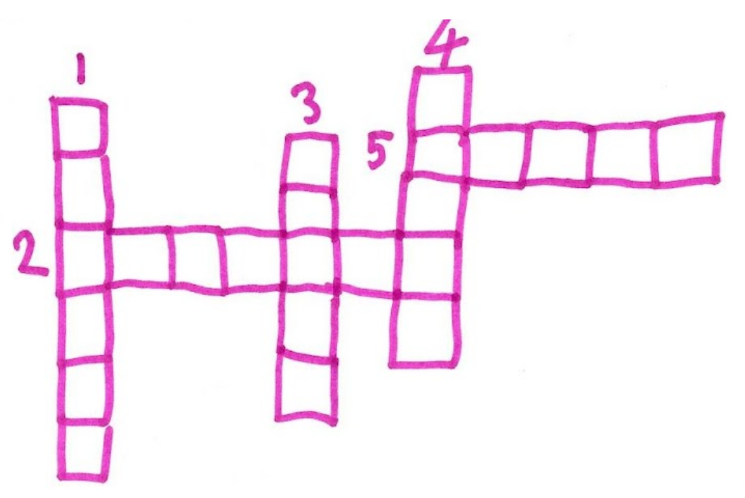
\includegraphics[width=0.5\textwidth]{assets/seikkailijat1}
\end{multicols}


\noindent\textbf{Vitsi aika!}\\
Mitä ruokaa voi syödä kuussa ja maassa? Kuumaa ruokaa!

\bigskip
\noindent\textbf{KYSYMYS!}\\
Jos kyltti kertoo että se on huijaus se tarkoittaa että se on totta, mutta jos se on totta se on totta että se on huijaus.\\
Tätä kutsutaa PARADOXIKSI!

\bigskip
\noindent Kuisma


% \noindent\textbf{Maailman huonoin vitsi!}\\
% Rusakko: No voi vitsit\\
% Puu: Eihän toi ollu vitsi\\
% Ilma: Toi on niin puinen vitsi että puu vastas siihen\\
% Ruoho: Lalala\\
% Lentävä lehmä joka ei näytä lehmältä: Muumaa mums!\\
% Epämuotoinen kukka: Lopeta jo tuolta tulee rusakko\\

% \bigskip
% \noindent Teksti ja kuva: Lillian

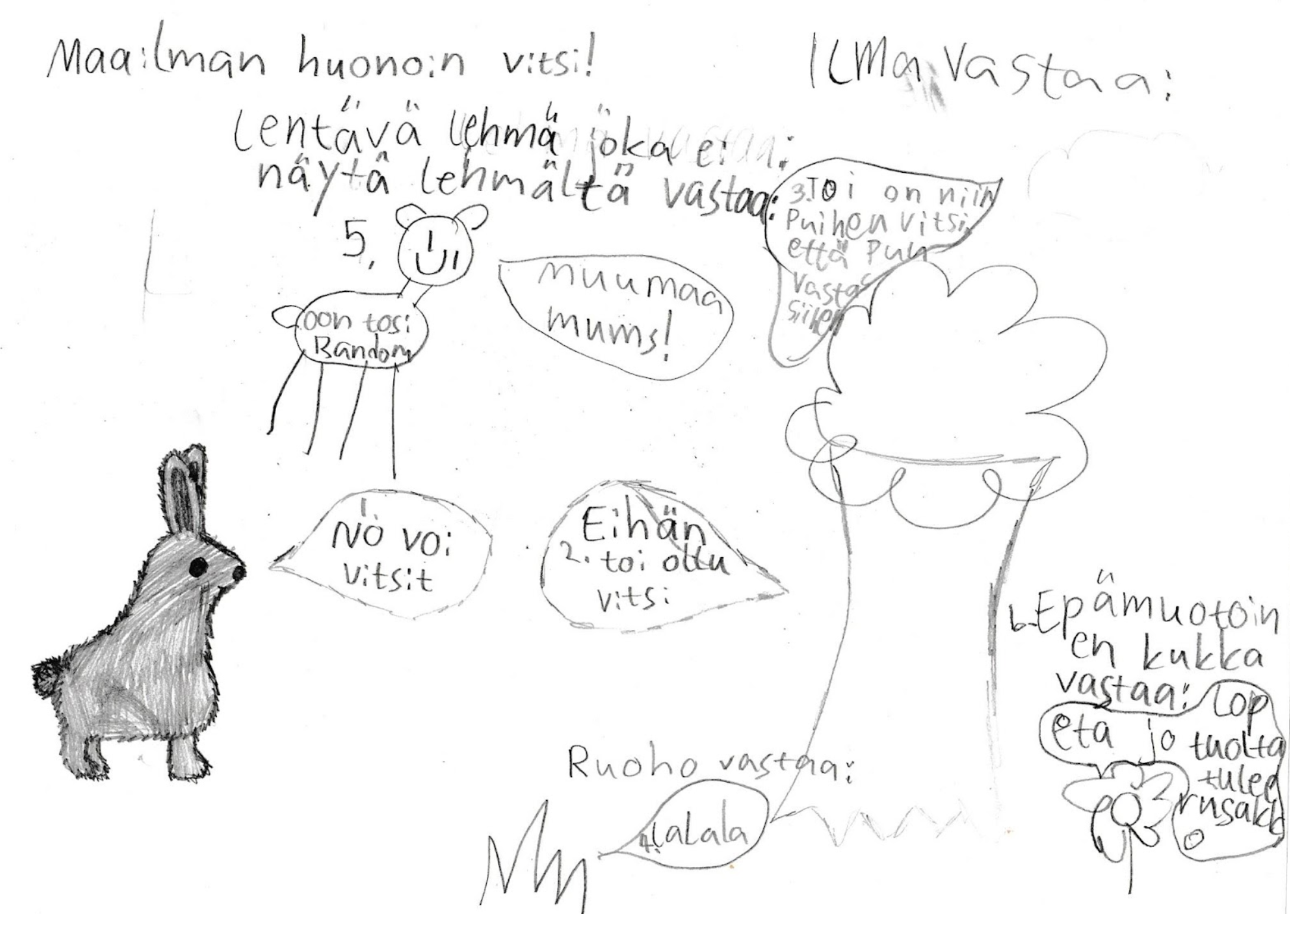
\includegraphics[width=1.0\textwidth]{assets/seikkailijat3}

\bigskip
\noindent Lillian

\bigskip
\hrule

\bigskip
\noindent\textbf{Vitsejä:}\\

\begin{multicols}{2}
\bigskip
\noindent“Mikä on nalle-puhin veli?”\\
“no?”\\
“puh-veli.”\\

\bigskip
\noindent“Kumpi ja Kampi tappelivat.”\\
“Kumpi voitti!”\\

\bigskip
\noindent“miksi darth vader meni \mbox{silmälääkäriin}?”\\
“no?”\\
“hän ei nähnyt Lukea”\\

\columnbreak

\bigskip
\noindent“miksi poliisin ei tarvi käydä \mbox{vessassa}?”\\
“no?”\\
“se pidättää kakkaa.”\\

\bigskip
\noindent“Montako kaksosia on?”\\
“no?”\\
“kaksi”.\\
\end{multicols}


\bigskip
\noindent Samuel


\begin{center}
\noindent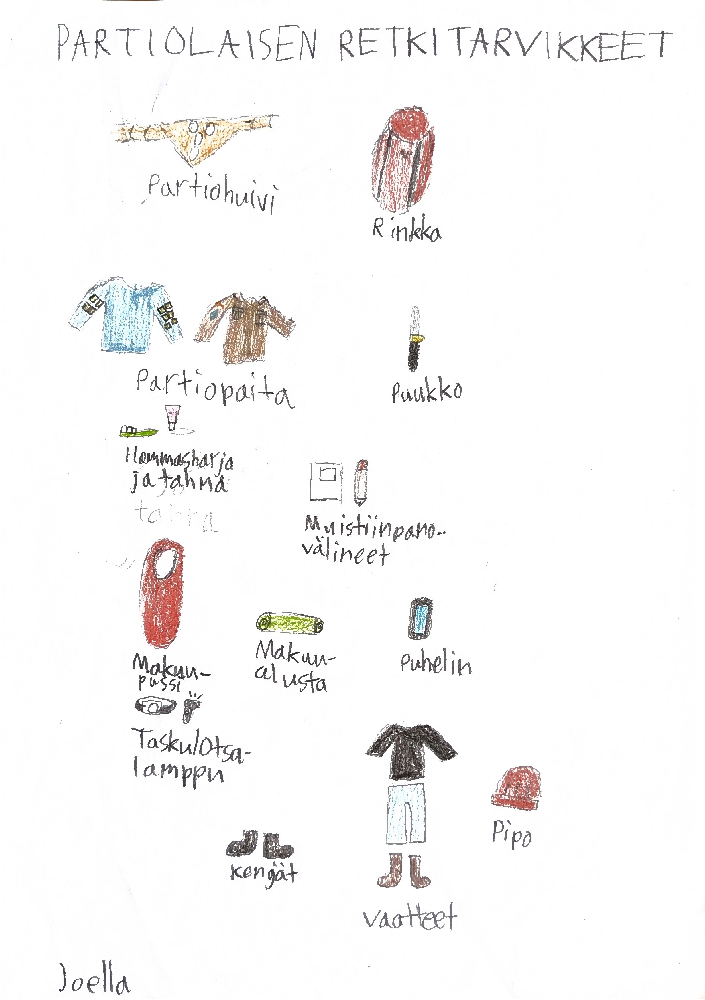
\includegraphics[width=1.0\textwidth,trim={0 0 0 0.5cm},clip]{assets/seikkailijat4}
\end{center}



%STORIES FROM RETKI/VAELLUS/LEIRI/EVENT
\section{Eläinten joulu Meriharjussa}

\textit{Gustaf Björkenheimin rakennuttama Villa Meriharju on vuonna 1910 
valmistunut huvila Uutelassa. Nykyään huvila on Helsingin kaupungin 
omistuksessa ja se kulkee nimellä Meriharjun luontotalo. Rusakot ovat tehneet 
pikkujouluretkiä luontotalolle jo useamman kerran, vuosina 1996--2001, 2003, 
2008, 2009, 2015, 2016 ja 2019--2023. Myös vuoden 2024 pikkujouluretki 
suuntautui Meriharjuun -- lue lisää retken tapahtumista tästä jutusta!}

\begin{figure}[!b]
\centering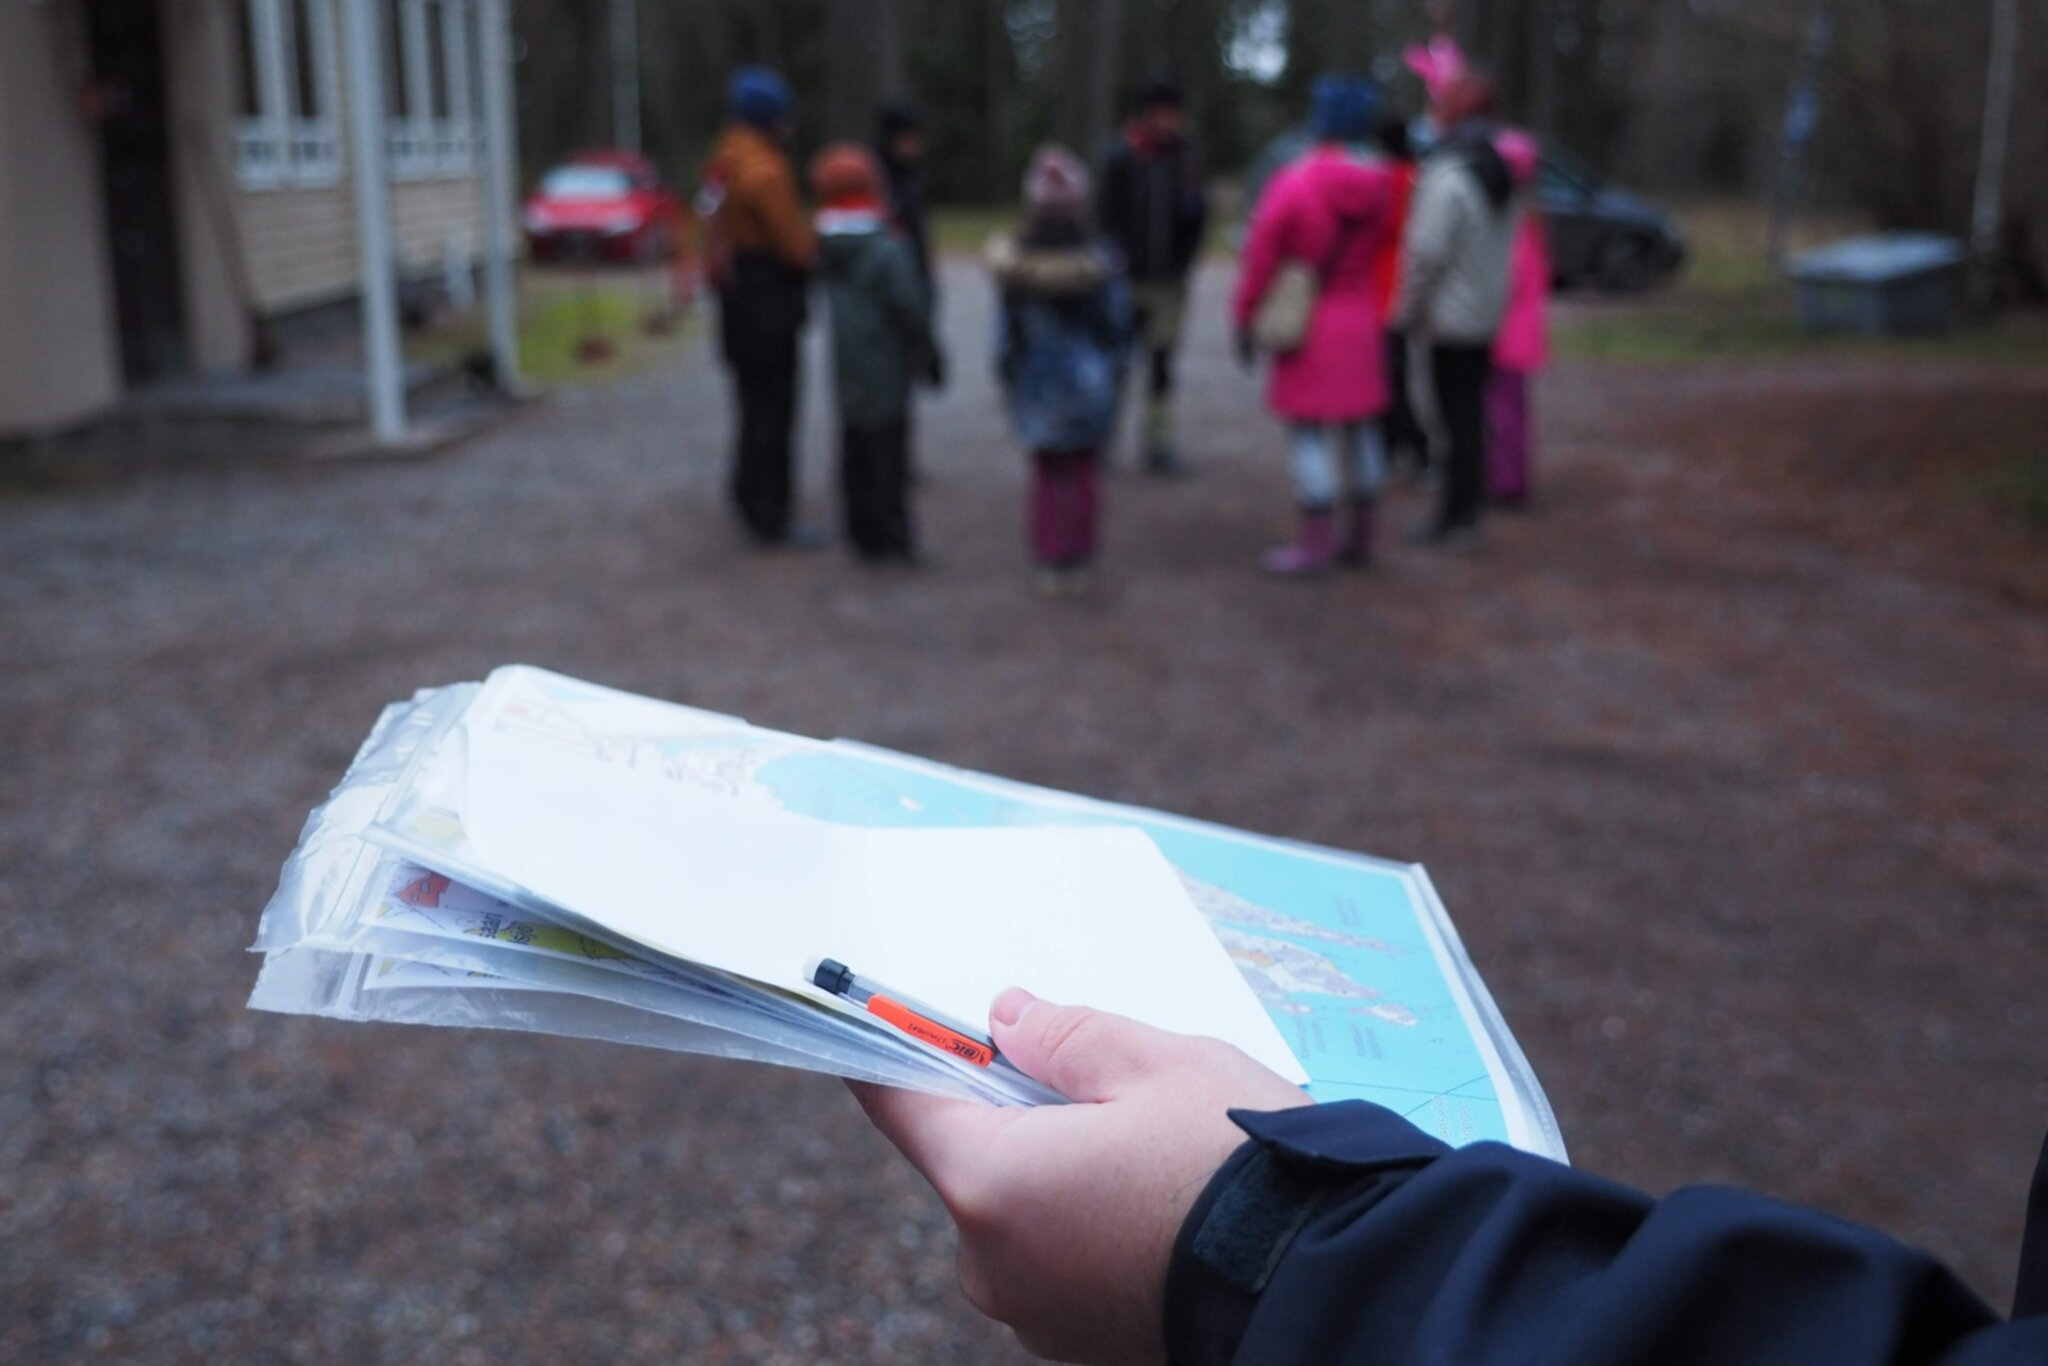
\includegraphics[width=\textwidth]{assets/meriharjuSuunnistus}
\caption{Lippukuntaretken lauantaisuunnistus käynnistyi luontotalon edustalta.}
\end{figure}

\begin{multicols}{2}
\noindent Kautta aikain rusakoiden pikkujouluretkillä on ollut erilaisia 
teemoja. Viime vuosina teemoina ovat olleet Itämeri, lentokykynsä 
menettäneet joulupukin porot, Kalevalan joulu sekä karanneet ja vilustuneet 
lehmät. Rusakoiden Meriharjun 17. pikkujouluretken teemana oli metsän 
eläinten joulu. 

\begin{figure*}[!t]
\centering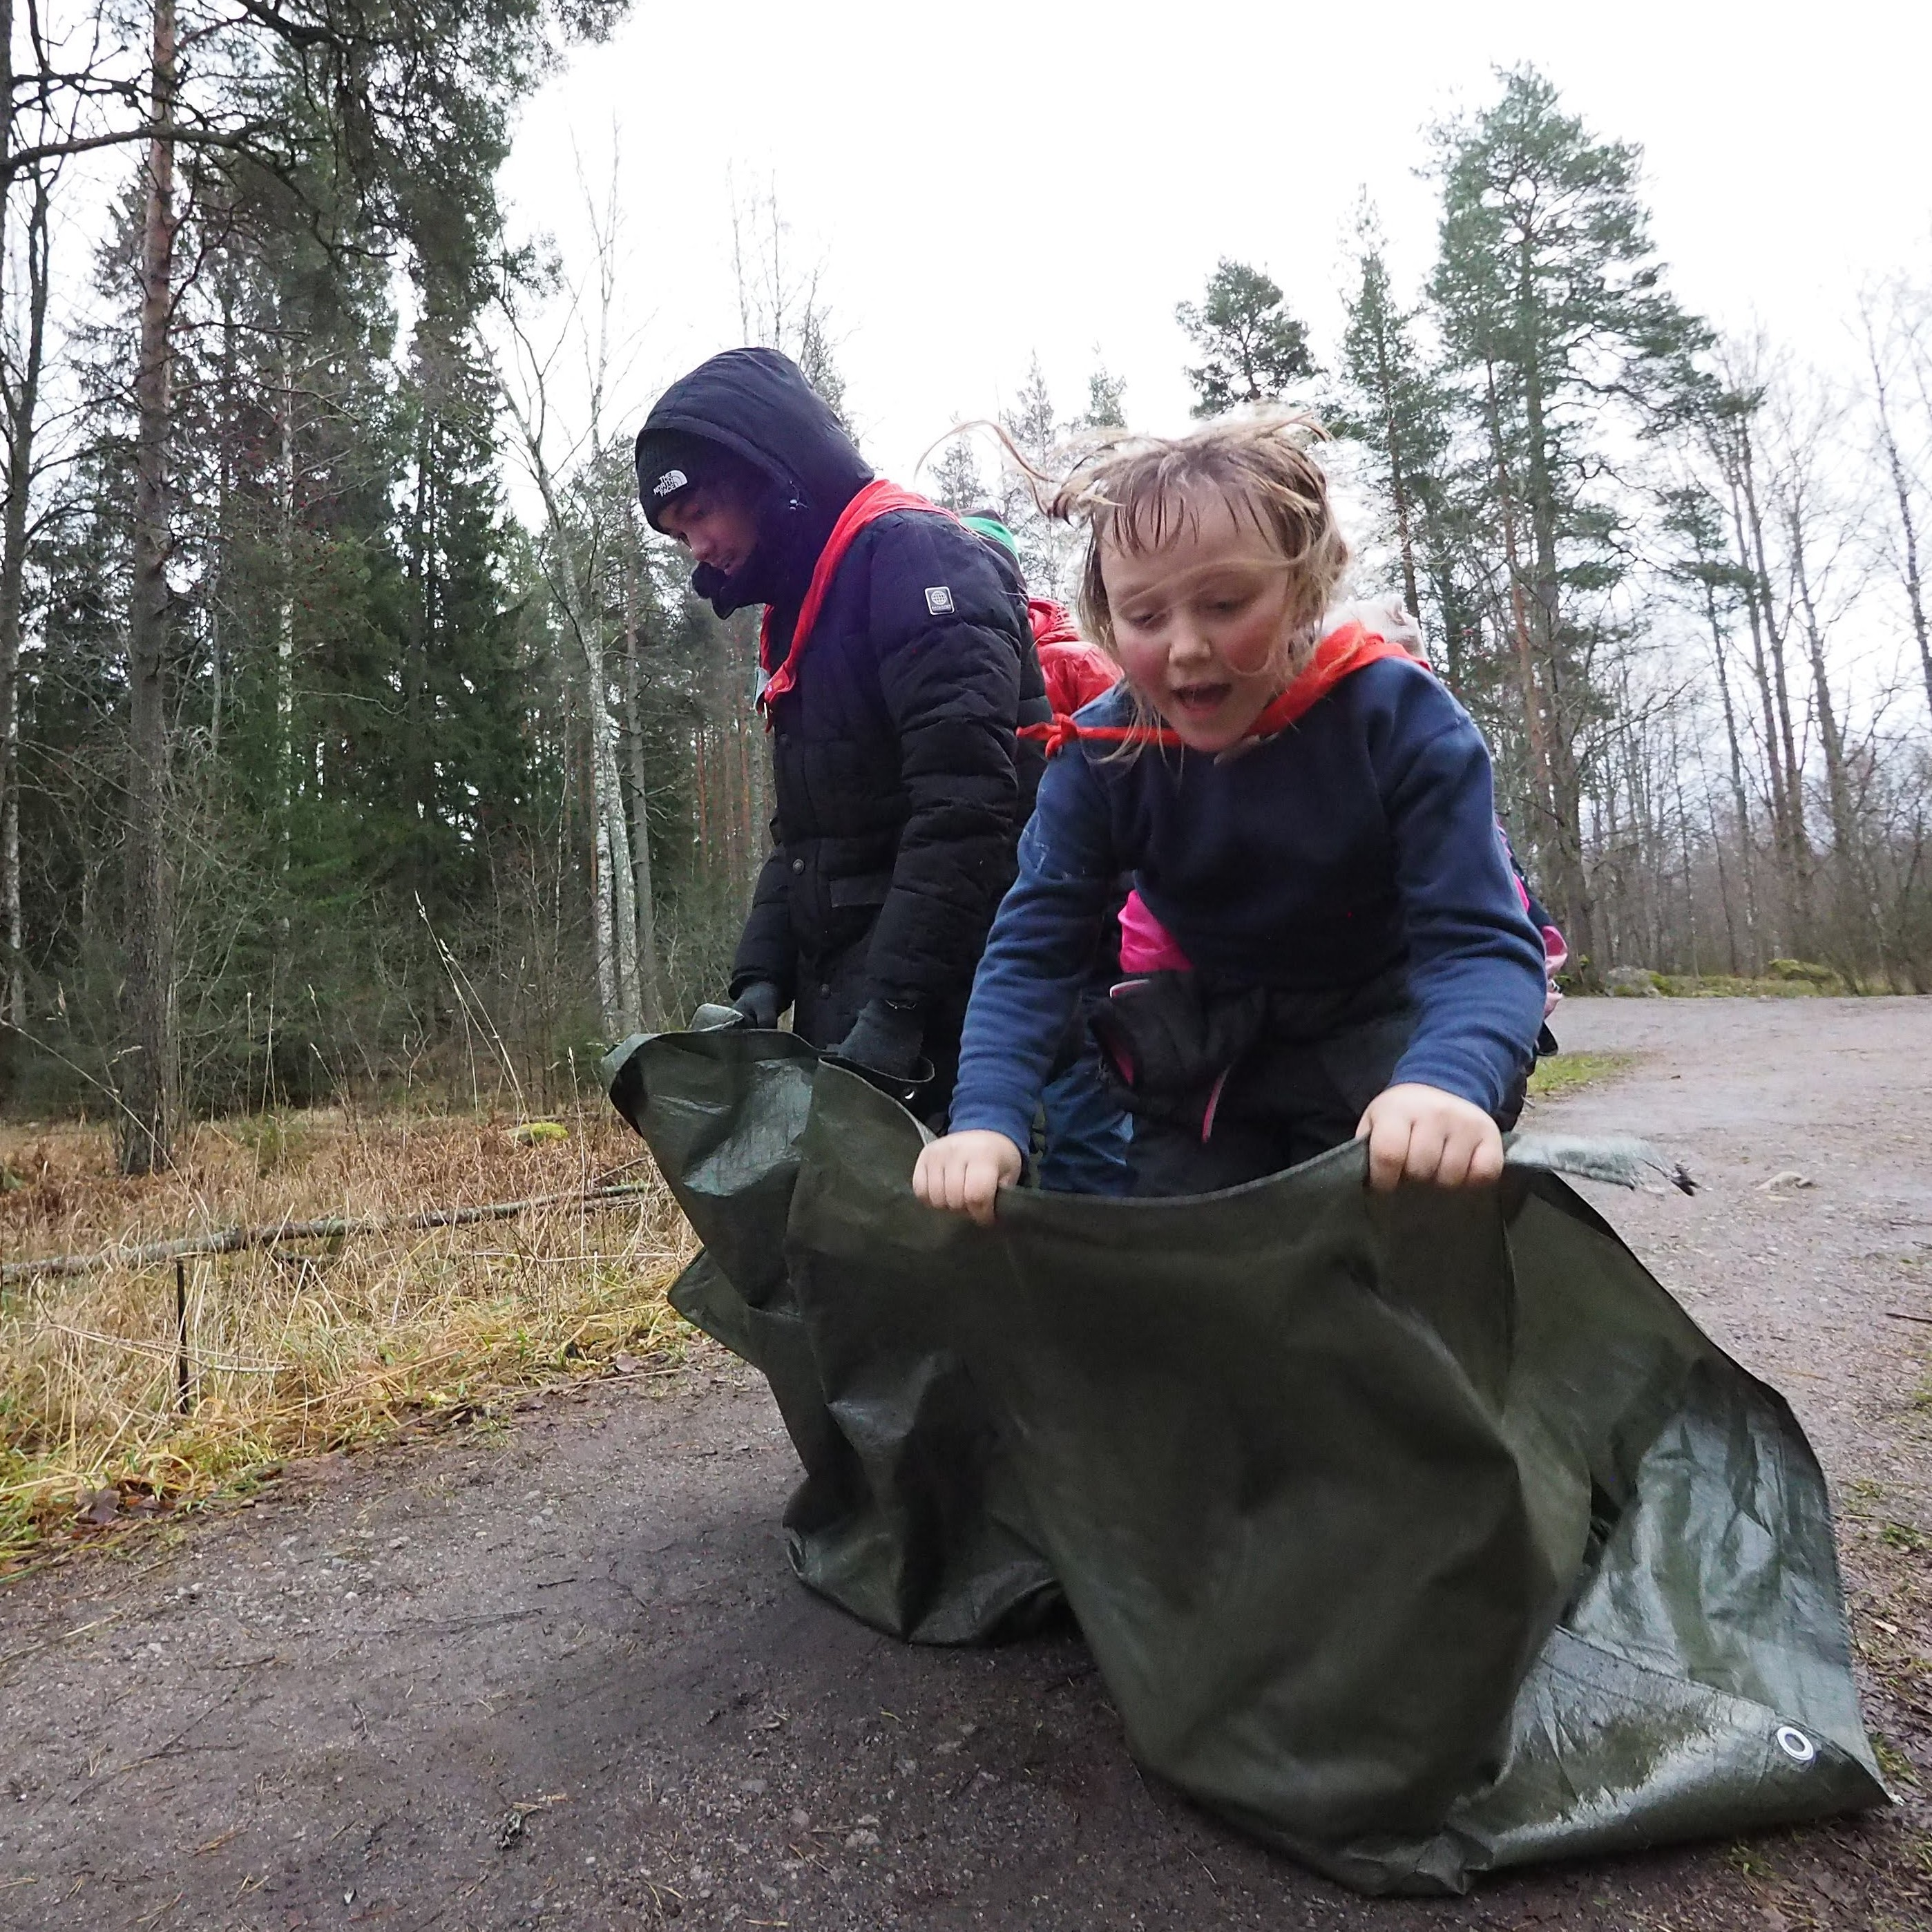
\includegraphics[width=.475\textwidth]{assets/meriharjuTaikamatto}\hfill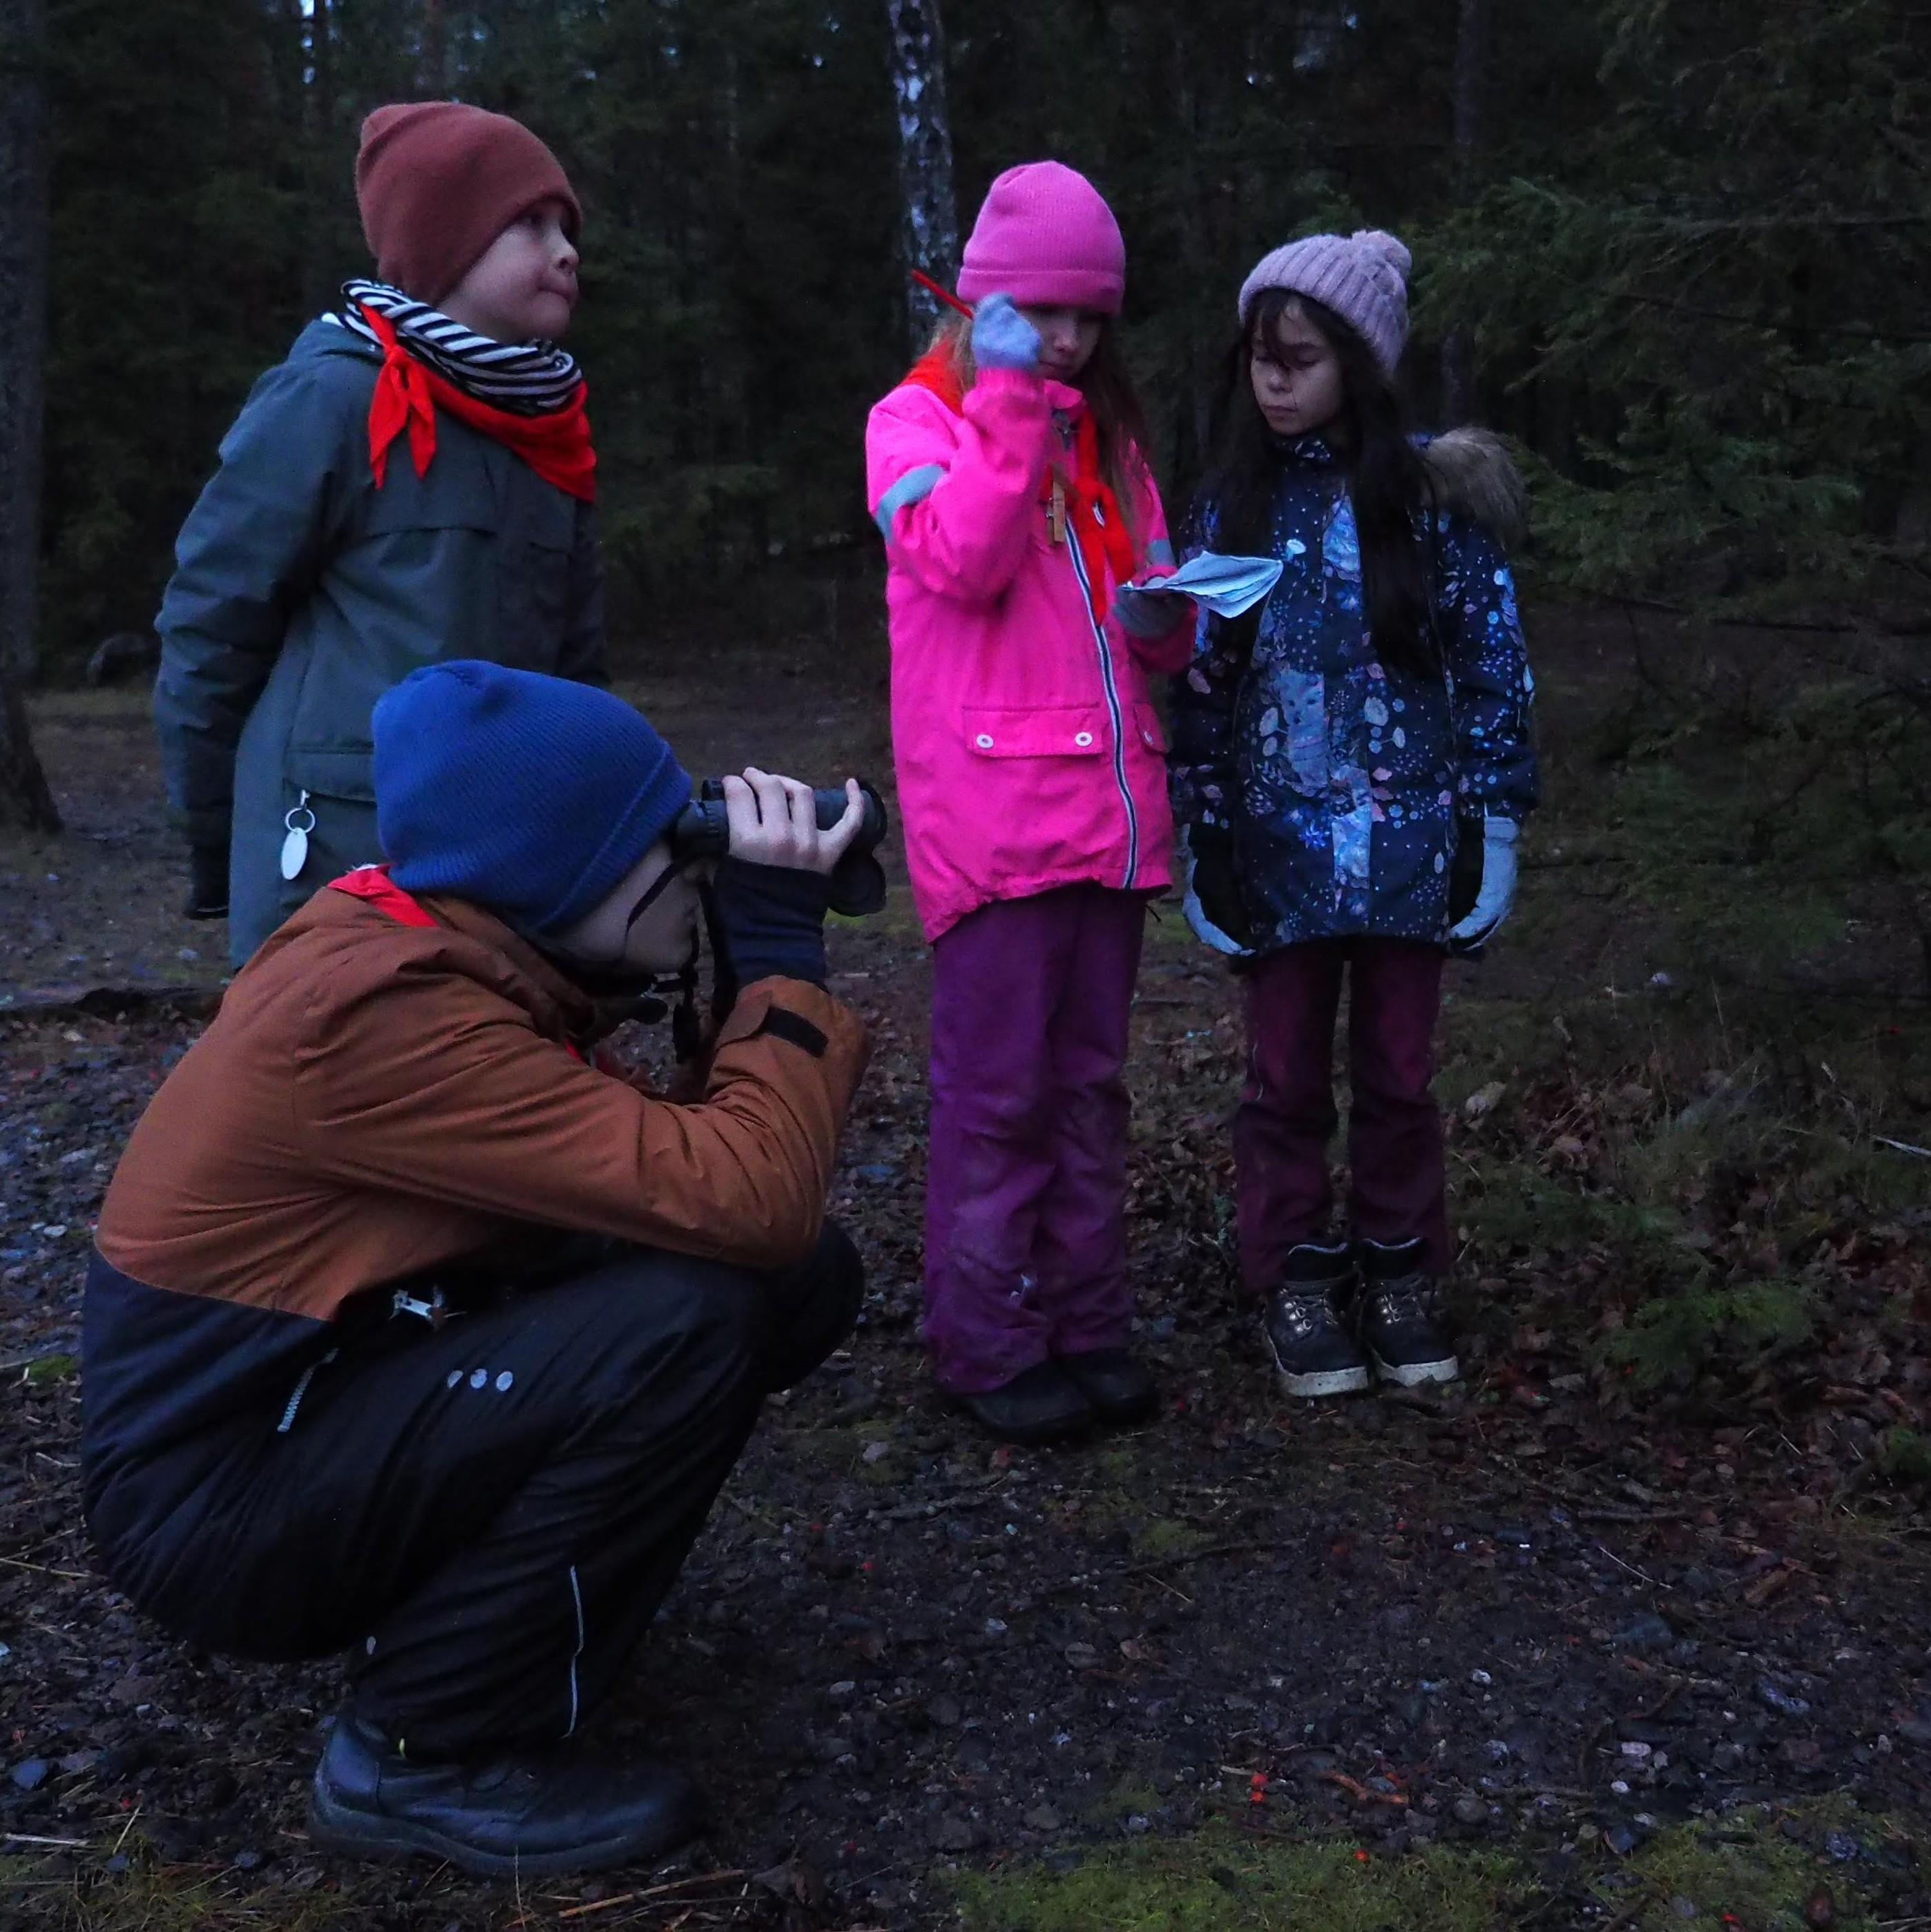
\includegraphics[width=.475\textwidth]{assets/meriharjuLinnut}
\caption{Neonvalo-vartio Kuusenalusmatto-rastilla ja Tyypit-vartio Poro, peura tai hirvi? -rastilla.}
\end{figure*}

Peräti 24 rusakkoa kokoontui jo tutuksi käyneellä bussilinja 560:n 
pysäkillä Kontulassa, josta matka jatkui kohti itää. Kävely Vuosaaren 
metroasemalta luontotalolle oli nuorempien retkeläisten mielestä 
jännittävä, kun viimeisellä kilometrillä ei ollutkaan enää 
katuvalaistusta. Tasku- ja otsalamput kaivettiinkin esiin hyvissä ajoin 
lyhyellä tauolla Sumujen sillalla. 

Kämpän pihalla vuorossa oli retkenjohtajan lyhyt ohjeistus ja Vene"-vartion 
leikkikimara ennen sisään siirtymistä ja majoittautumista: uniikki, 
sisäkissa"-ulkokissa ja lännen nopein. Kolkat yöpyisivät yhdessä 
huoneessa, seikkailijat ja tarpojat toisessa, samoajat ja Nonna kolmannessa ja 
muut johtajat neljännessä huoneessa. Retken kokonaisvahvuus oli 33 eli kaikki 
sänkypaikat paitsi yksi tulivat käytettyä.

Voileipäiltapalan jälkeen siirryttiinkin jo iltatoimille ja nukkumaan. Osa 
seikkailijoista ja tarpojista jäi vielä hetkeksi valvomaan takahuoneeseen ja 
osa johtajista kävi perjantaisaunassa.

Lauantaiaamu käynnistettiin kaurapuurolla ja pian oli aika suunnistukselle. 
Matkaan lähti viisi vartiota: Sudet, Neonvalo, Pupunkorvat, Tyypit ja 
S.U.P.E.R.G.A.L.A.K.T.I.S.E.T. F.E.M.I.N.I.S.T.I.M.A.R.S.U.T. (lyhyemmin 
S.G.F.M.). Rastikiertoon liittyi retken teemaan sopiva kehystarina, joka 
mukaili Marketta Pyysalon kertomusta \textit{Siili, jonka joulu herätti}. 

Suunistuksen ensimmäisellä rasteilla tunnistettiin eläinten lumijälkiä. 
Valitettavasti retkilauantaina ei vielä lunta maassa ollut, minkä vuoksi 
jälkien tunnistus tapahtui puhelimen näytöltä. Toisella rastilla vartion 
tehtävänä oli edetä pressun päällä rastihenkilön määräämä matka ja 
kolmannella laulaa joululauluja, joissa esiintyi tiettyjä sanoja. Neljäs 
rasti sijaitsi Niemenapajalla, jossa vartio etsi kertakäyttölusikoita 
maastosta.

\begin{figure*}[!t]
\centering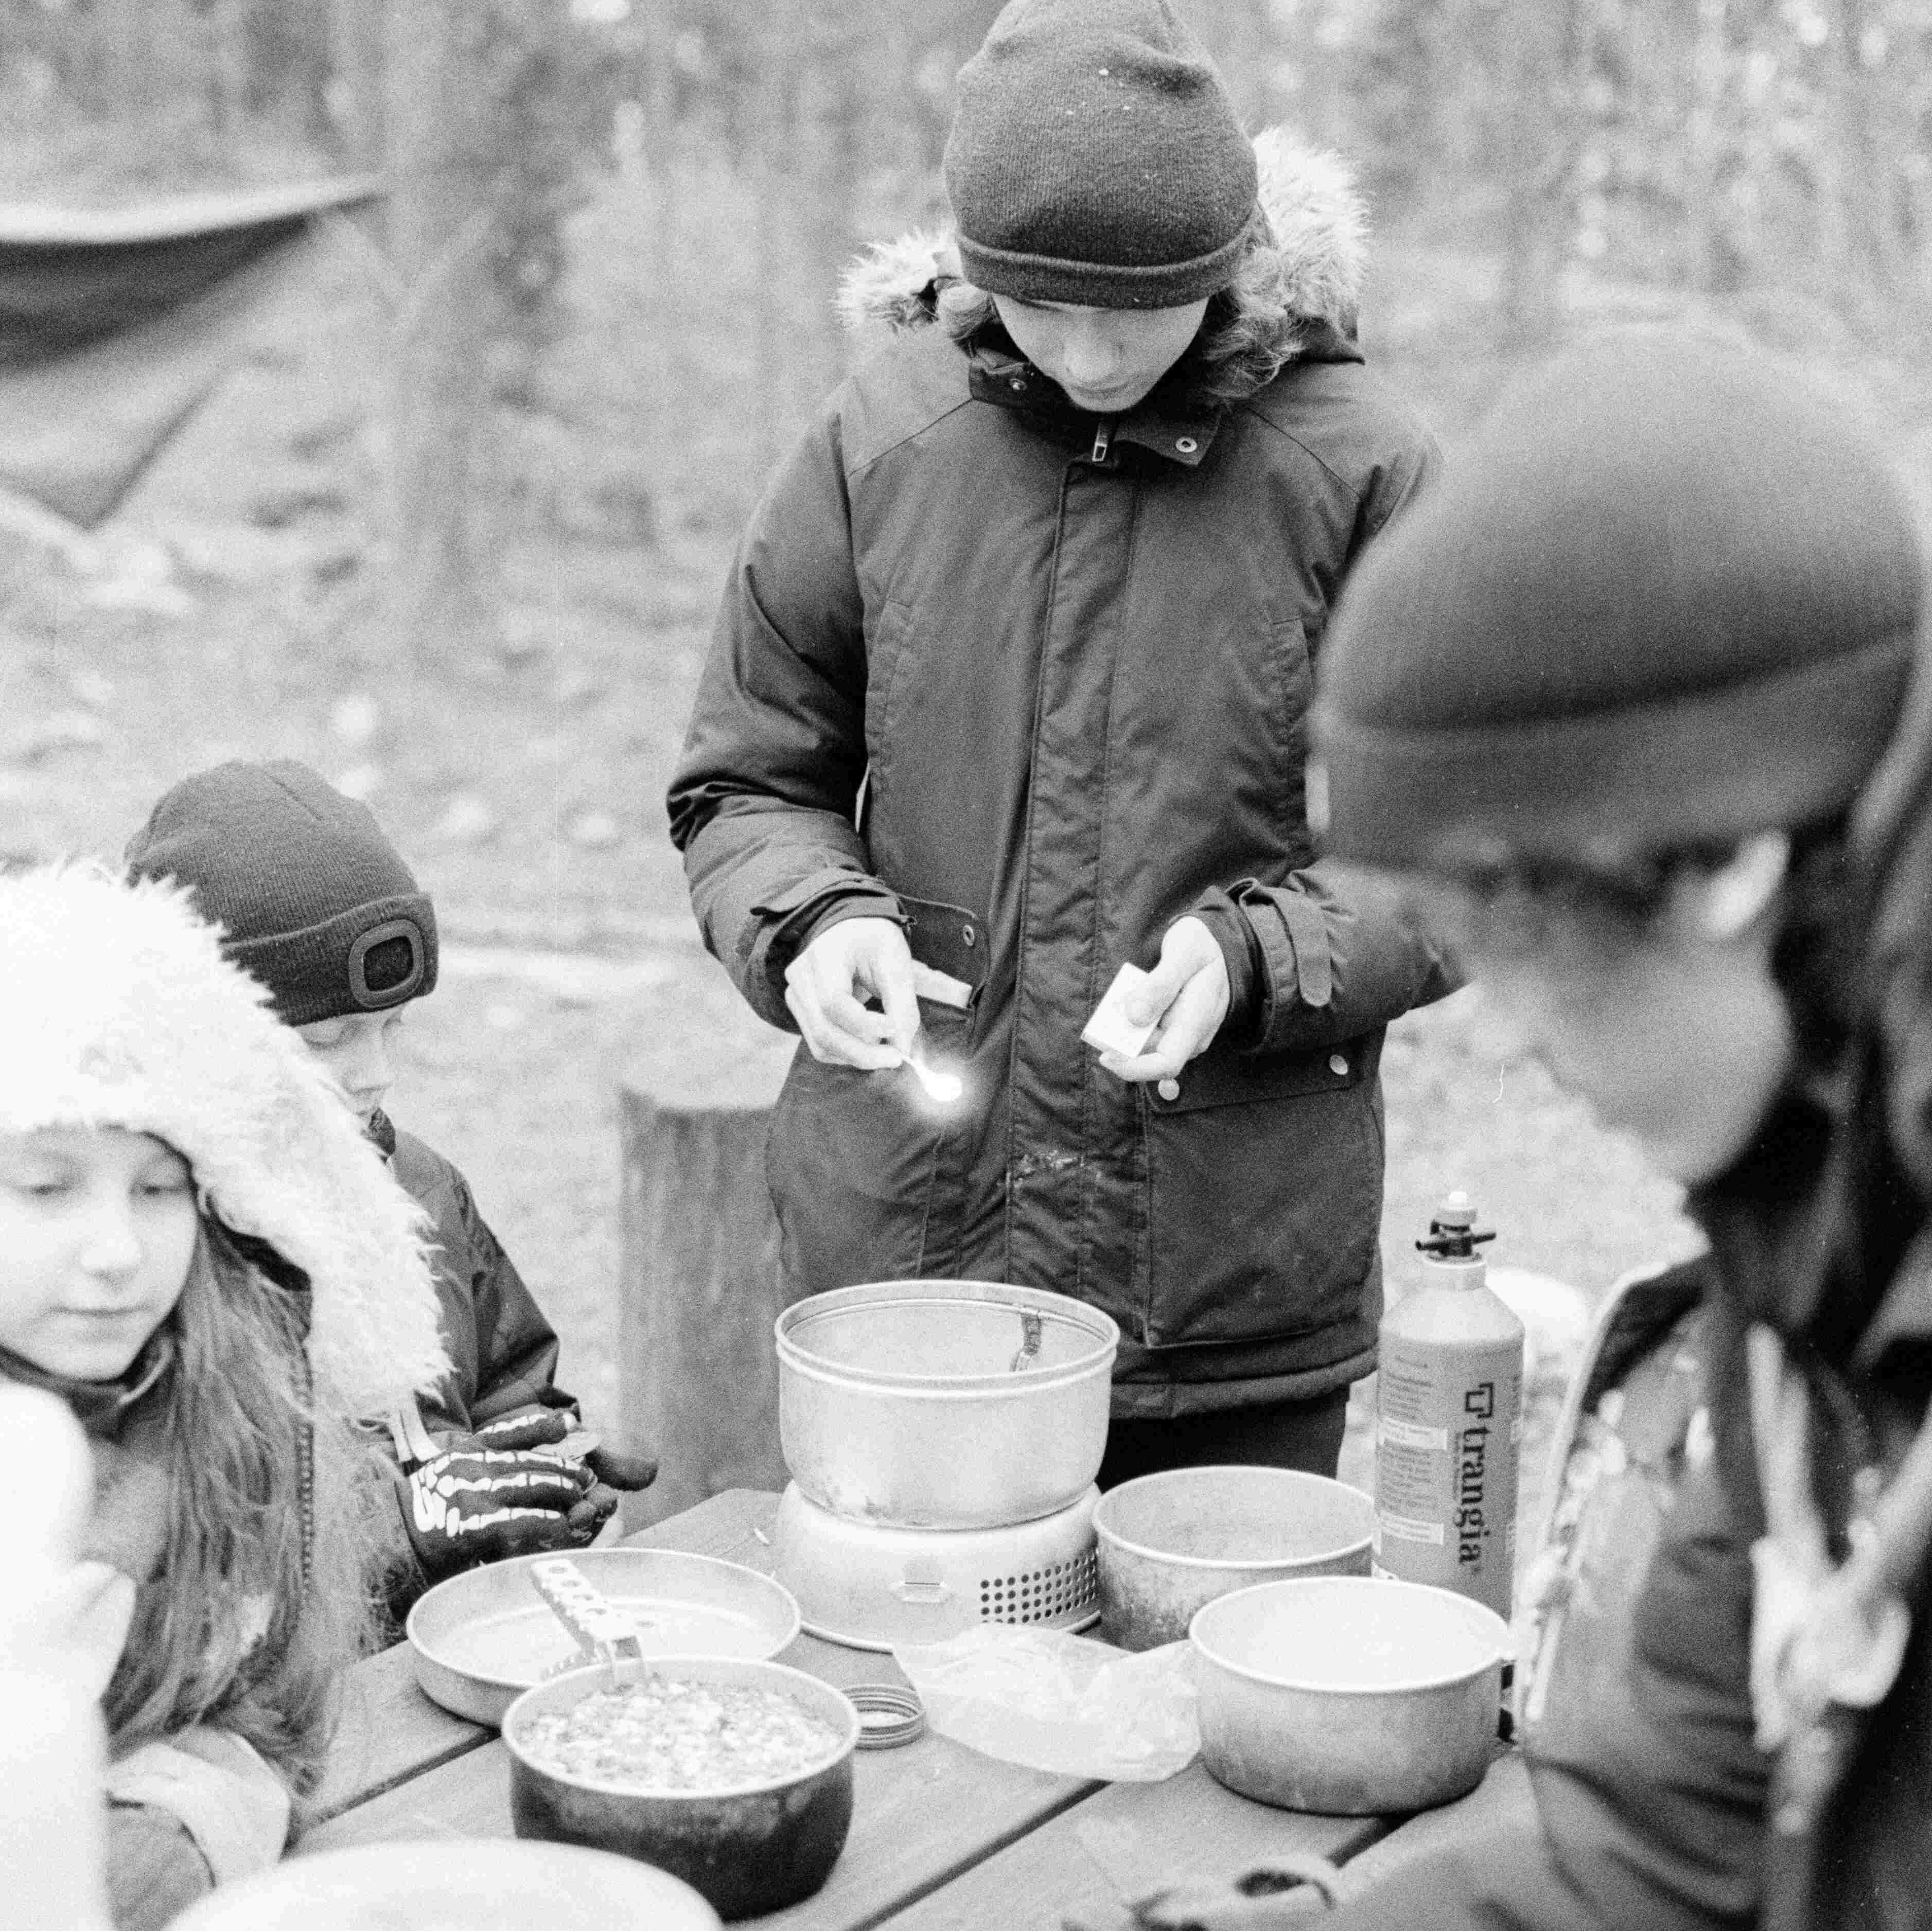
\includegraphics[width=.475\textwidth]{assets/meriharjuRuoka1}\hfill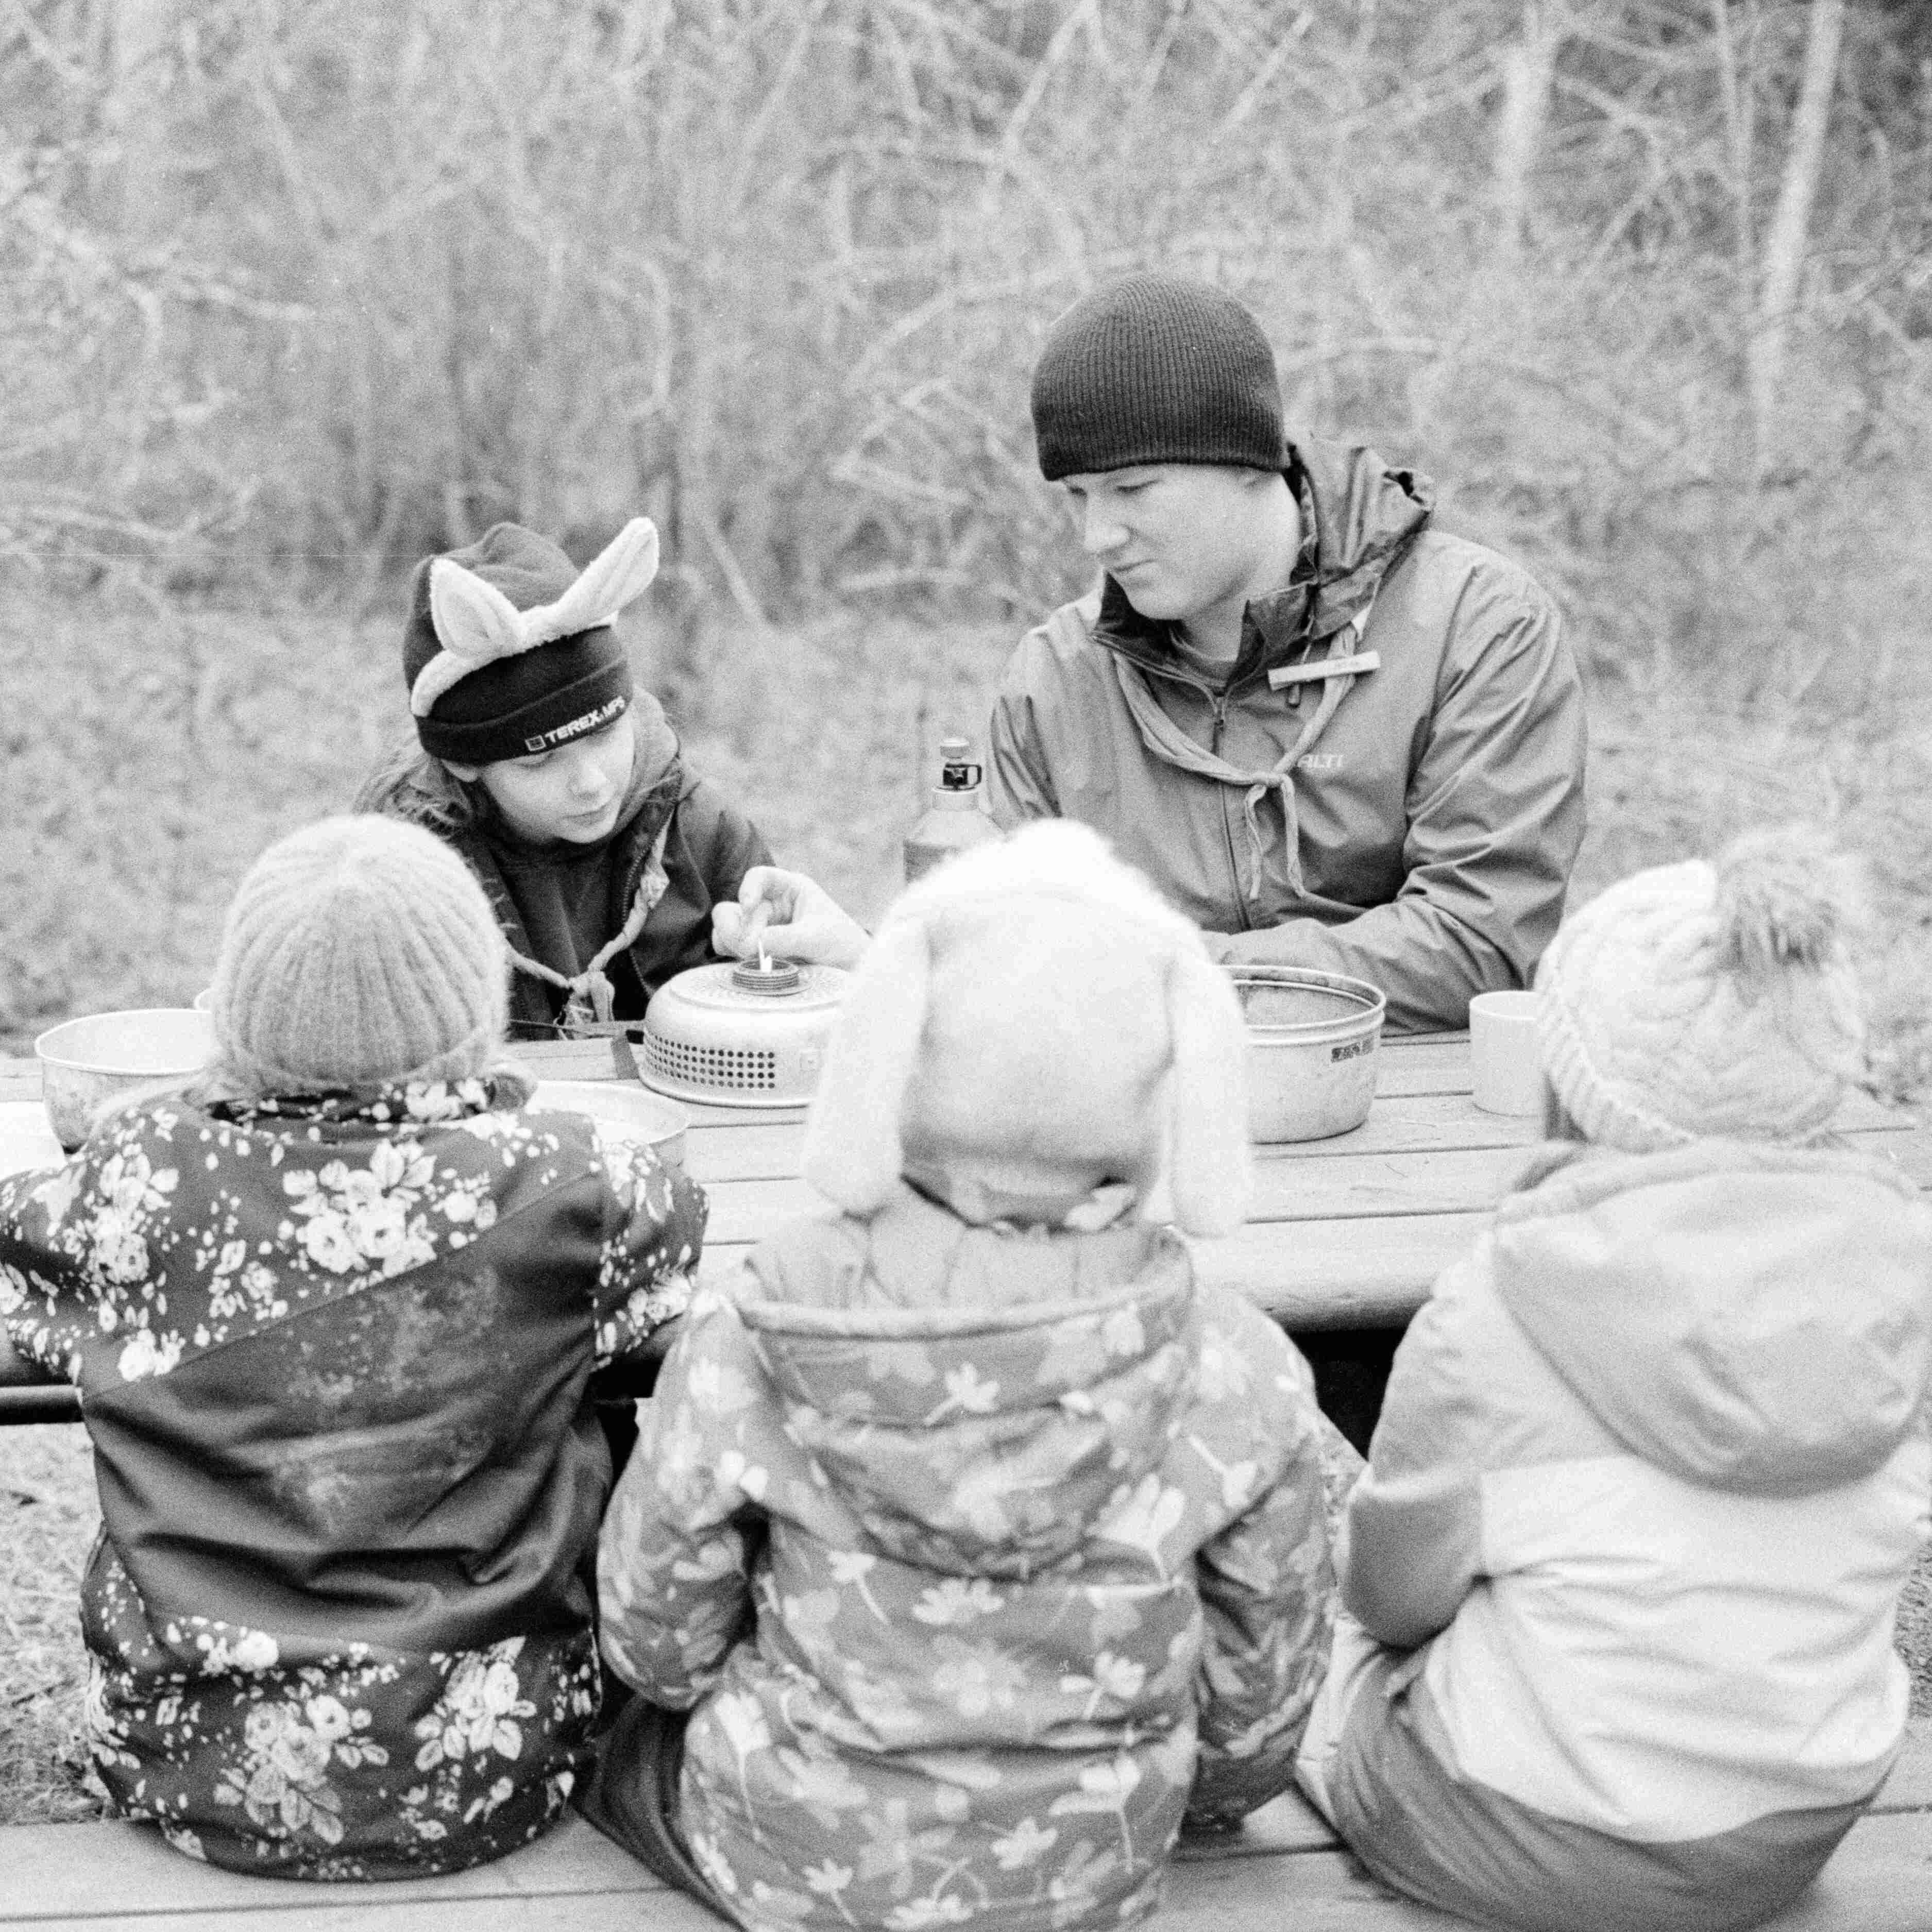
\includegraphics[width=.475\textwidth]{assets/meriharjuRuoka2}
\caption{Sudet- ja Pupunkorvat -vartiot ruokarastilla.}
\end{figure*}

Vielä oli kaksi rastia jäljellä, mutta ennen niitä vartiot valmistivat 
itselleen maittavan trangialounaan: tonnikalanuudeleita, nams! Tässä 
vaiheessa alkoi sataa vähän räntää, mutta se ei vartoiden menoa haitannut. 
Kuudennella rastilla tehtiin iso merimiessolmu ja seitsemännellä rastilla 
tunnistettiin eläimiä. Maalitehtävä oli muita rastitehtäviä huomattavasti 
haastavampi, kun vartioiden piti yhdistää maakunnan vaakuna sitä vastaavaan 
maakuntamaaeläimeen, "=lintuun tai "=kalaan. 

Vaikka varsinaisia suunnistuksia ei viime lippukuntaretkillä ole ollutkaan 
ohjelmassa, kaikki vartiot löysivät hienosti kaikille rasteille. Seitsemän 
rastin, vajaan kahdeksan kilometrin suunnistukseen meni nopeimmalta vartiolta 
noin viisi tuntia ja hitaimmalta kuusi tuntia. Nopeudesta ei saanut pisteitä, 
mutta rastitehtävät pisteytettiin -- löydät vartoiden pisteytykset 
jutun lopun taulukosta. Onneksi olkoon, Tyypit!

Samaa vauhtia kuin vartiot saapuivat suunnistuksen maaliin vartiot alkoivat 
suunnitella omia piparkakkutalojaan. Kukin vartio sai käyttöönsä kokonaisen 
kilon piparkakkutaikinaa, josta tarkoituksena oli rakentaan kullekin vartiolle 
mieluisa teos. Varsin moni vartio rakensi perinteikästä piparkakkutaloa 
mukailevan rakennelman, mutta myös jännittävämpiä ratkaisuja kuten 
piparkakkunelitahokas ja piparkakkupelikortit nähtiin. Myös teokset 
pisteytettiin.

\begin{figure*}[!t]
\centering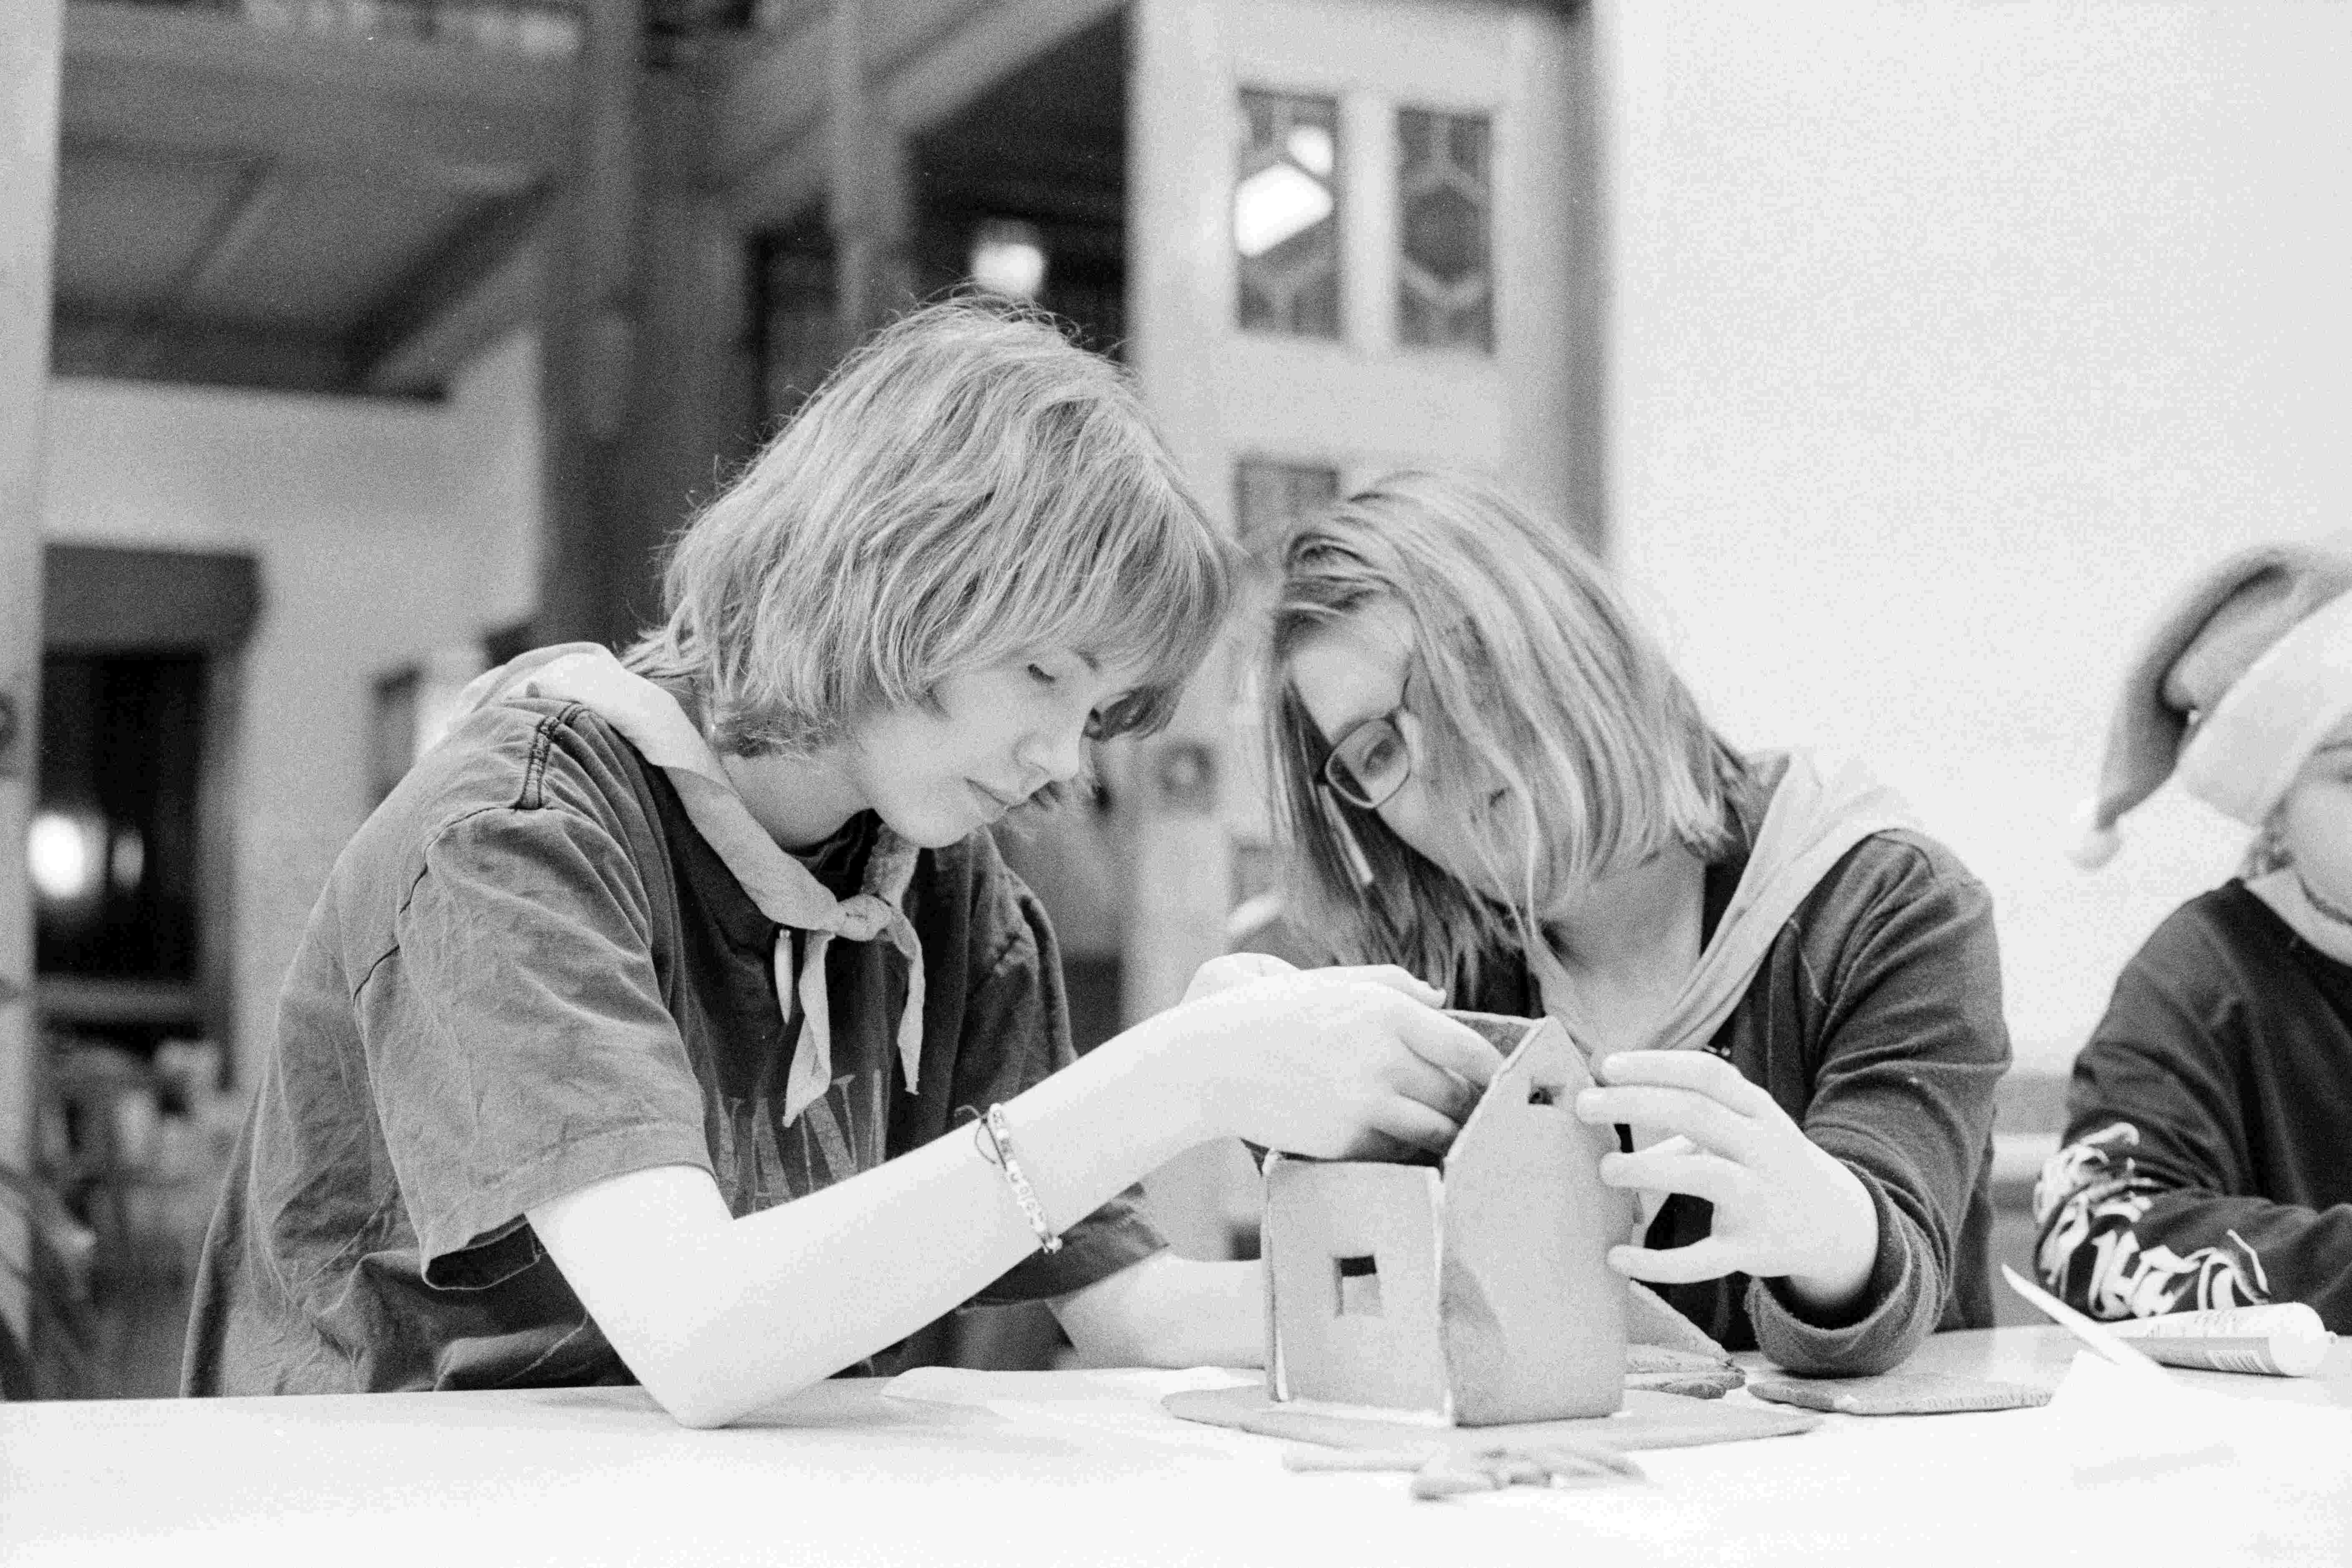
\includegraphics[width=\textwidth,trim={0 0 0 5cm},clip]{assets/meriharjuPipari}
\caption{S.U.P.E.R.G.A.L.A.K.T.I.S.E.T. F.E.M.I.N.I.S.T.I.M.A.R.S.U.T. -vartio rakentamassa piparkakkutaloa.}
\end{figure*}

\begin{table*}[b]\centering\small
\begin{tabular}{|l|c|c|c|c|c|}
\hline
 & \textbf{Tyypit} & 
\begin{tabular}[x]{@{}c@{}}\textbf{Pupun-}\\\textbf{korvat}\end{tabular} & 
\begin{tabular}[x]{@{}c@{}}\textbf{Neon-}\\\textbf{valo}\end{tabular} & 
\textbf{Sudet} & \textbf{S.G.F.M.} \\ \hline
\textbf{Lumijälkiä} & 3,00 & 3,00 & 1,00 & 3,00 & 5,00 \\ \hline
\textbf{Kuusenalusmatto} & 13,12 & 12,14 & 11,82 & 11,46 & 0,00 \\ \hline
\textbf{Kauneimmat joululaulut} & 10,00 & 8,00 & 7,00 & 2,00 & 6,00 \\ \hline
\begin{tabular}[x]{@{}c@{}}\textbf{Pata-himmeli 
ja}\\\textbf{ruutu-kranssi}\end{tabular} & 3,00 & 5,00 & 3,00 & 4,00 & 5,00 \\ 
\hline
\textbf{Joulurusetti} & 5,00 & 5,00 & 4,00 & 4,00 & 5,00 \\ \hline
\textbf{Poro, peura tai hirvi?} & 4,00 & 6,00 & 3,00 & 5,50 & 3,00 \\ \hline
\textbf{Joulun taikaa} & 25,00 & 12,50 & 25,00 & 12,50 & 12,50 \\ \hline
\textbf{Piparkakkutalot} & 30,00 & 35,00 & 24,00 & 35,00 & 37,00 \\ \hline \hline
 & 93,12 & 86,64 & 78,82 & 77,46 & 73,50 \\ \hline
\end{tabular}
\end{table*}

Piparkakkuteosten osien paistuessa syötiin herkullista kanapataa. 
Päivällisen jälkeen halukkaat kävivät saunomassa muiden laulaessa 
joululauluja ja koristellessa teoksiaan. Iltapalaksi oli jotain hieman 
erikoisempaa: nyhtöleipää, keksejä ja paukkumaissia!

Sunnuntaiaamu käytettiin pakkaamiseen ja siivoamiseen. Uusille kolkille 
järjestettiin kolkkakoe, jonka kaikki kolme kokelasta läpäisivät. Lounaaksi 
juuri ennen joulujuhlaa syötiin riisipuuroa. 

\begin{figure*}[p]
\centering
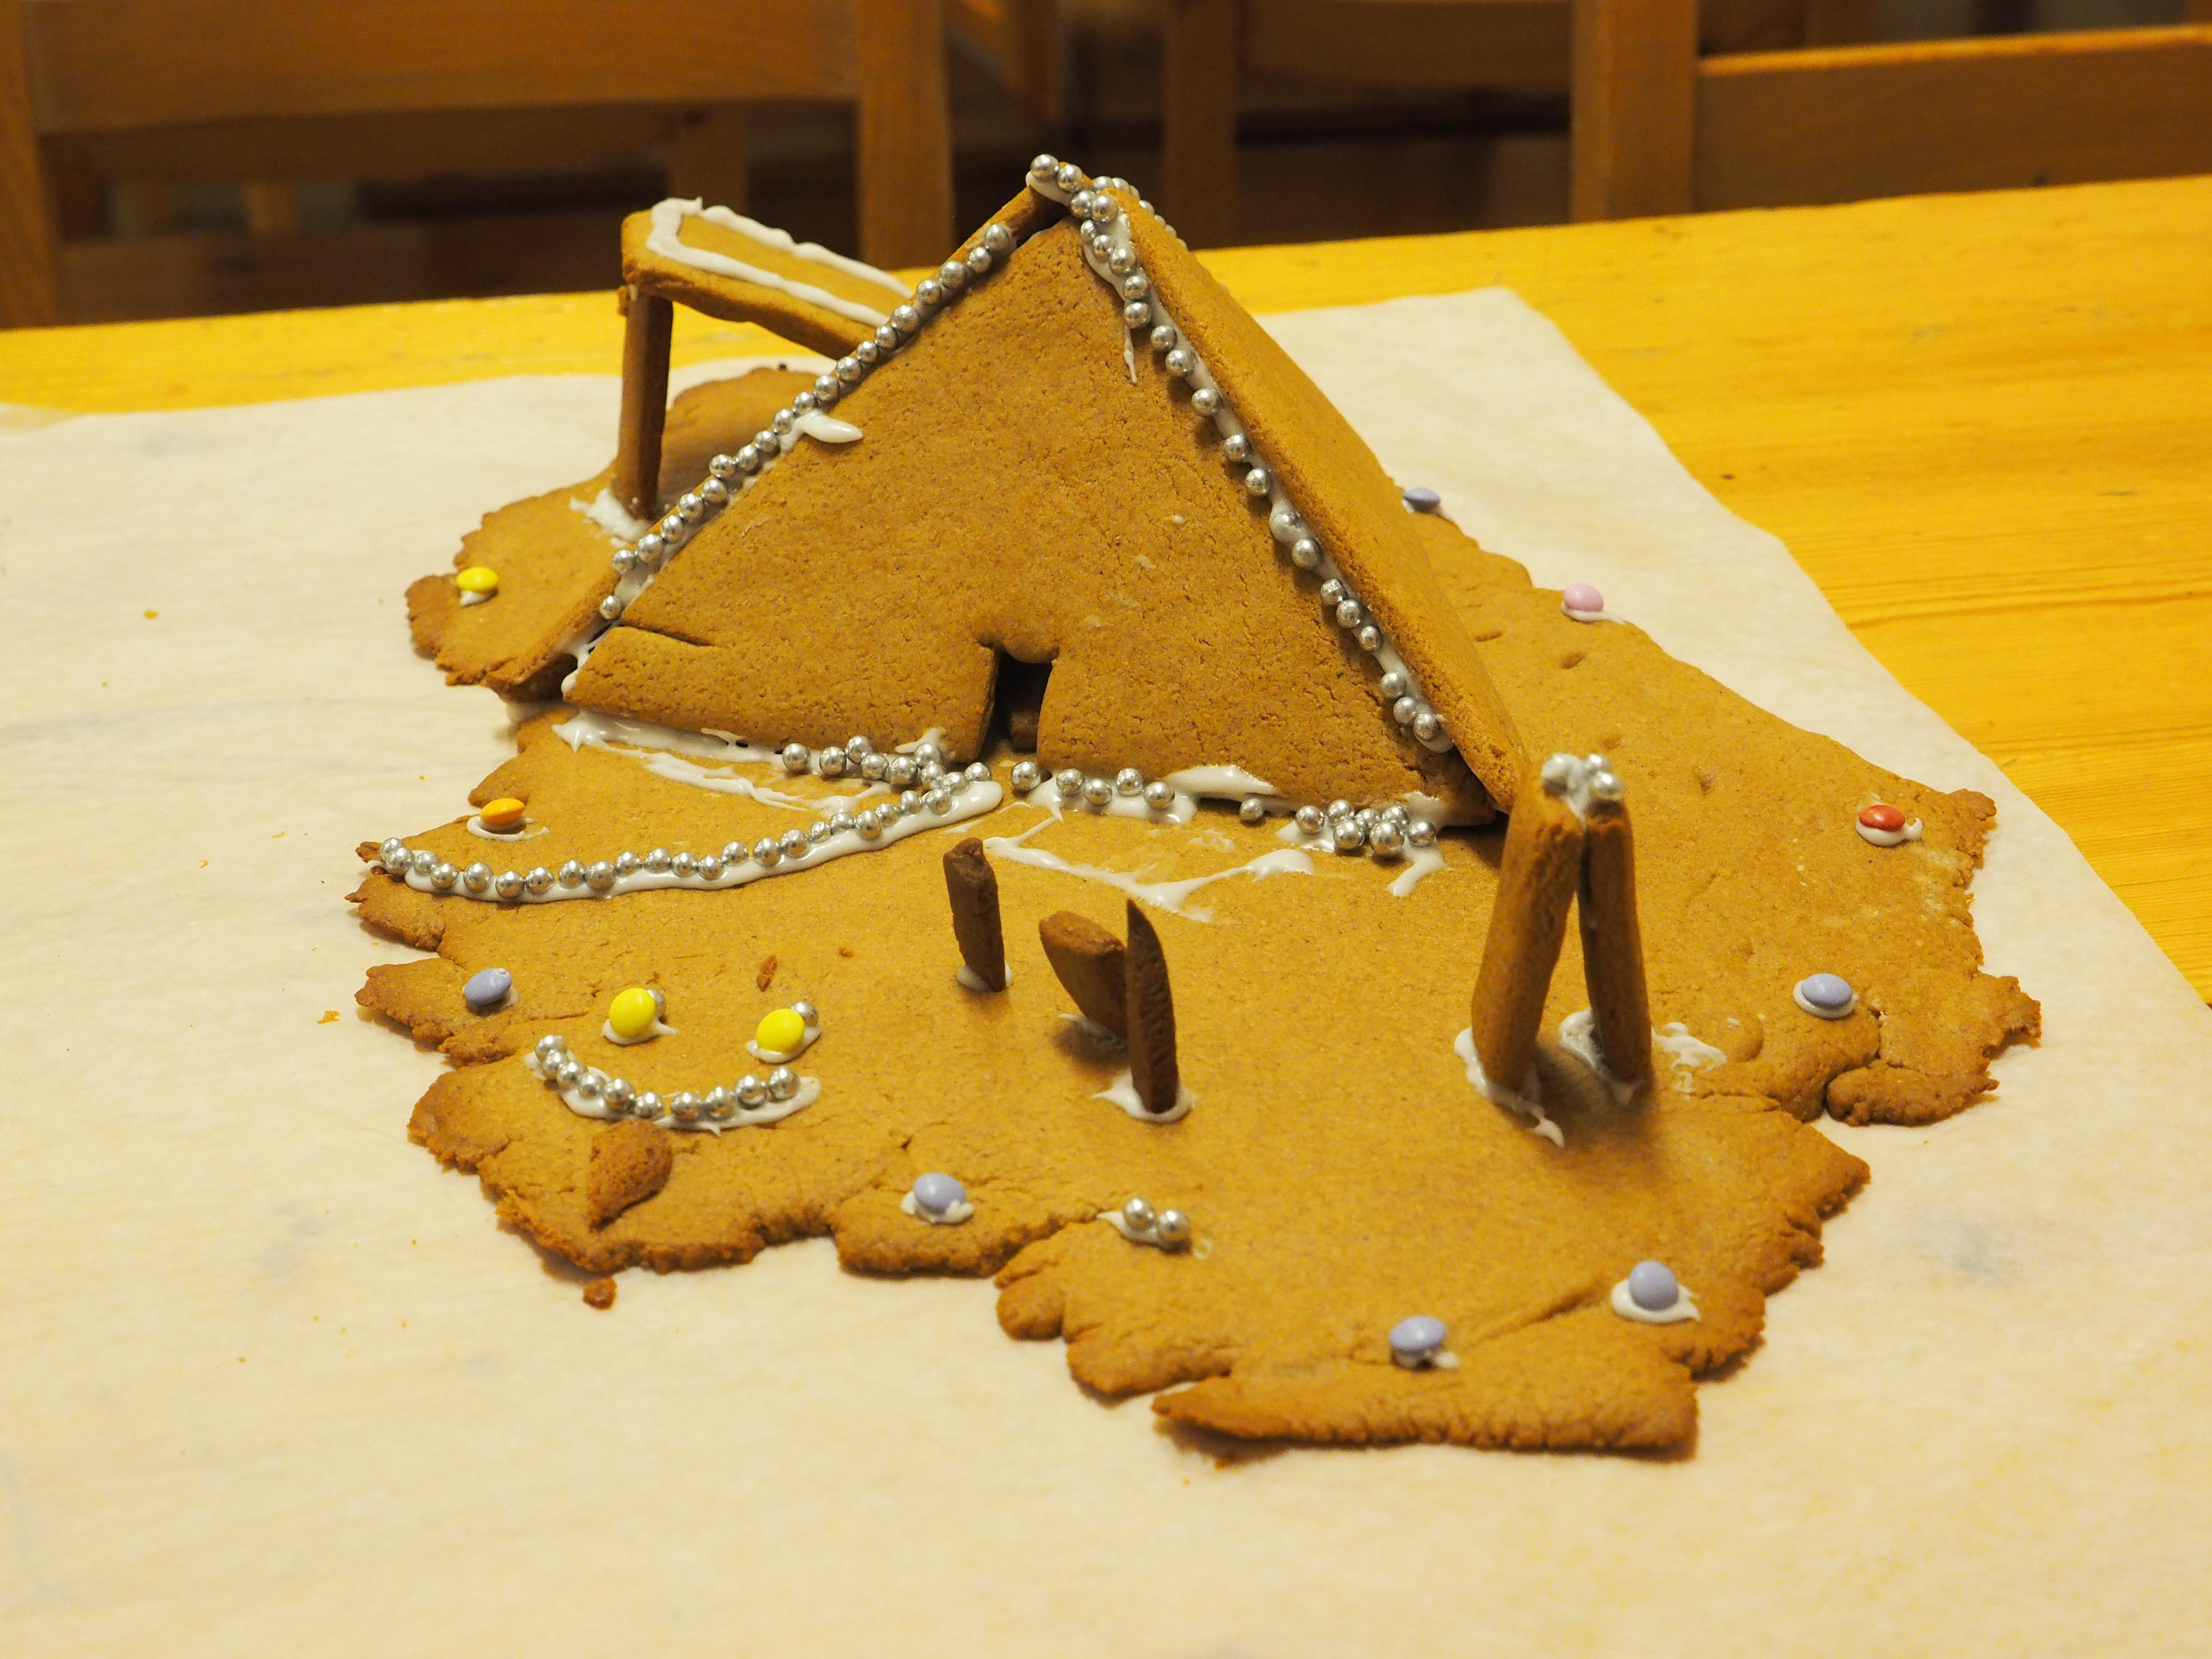
\includegraphics[width=.475\textwidth,height=.475\textwidth,keepaspectratio]{assets/pipari1}\hfill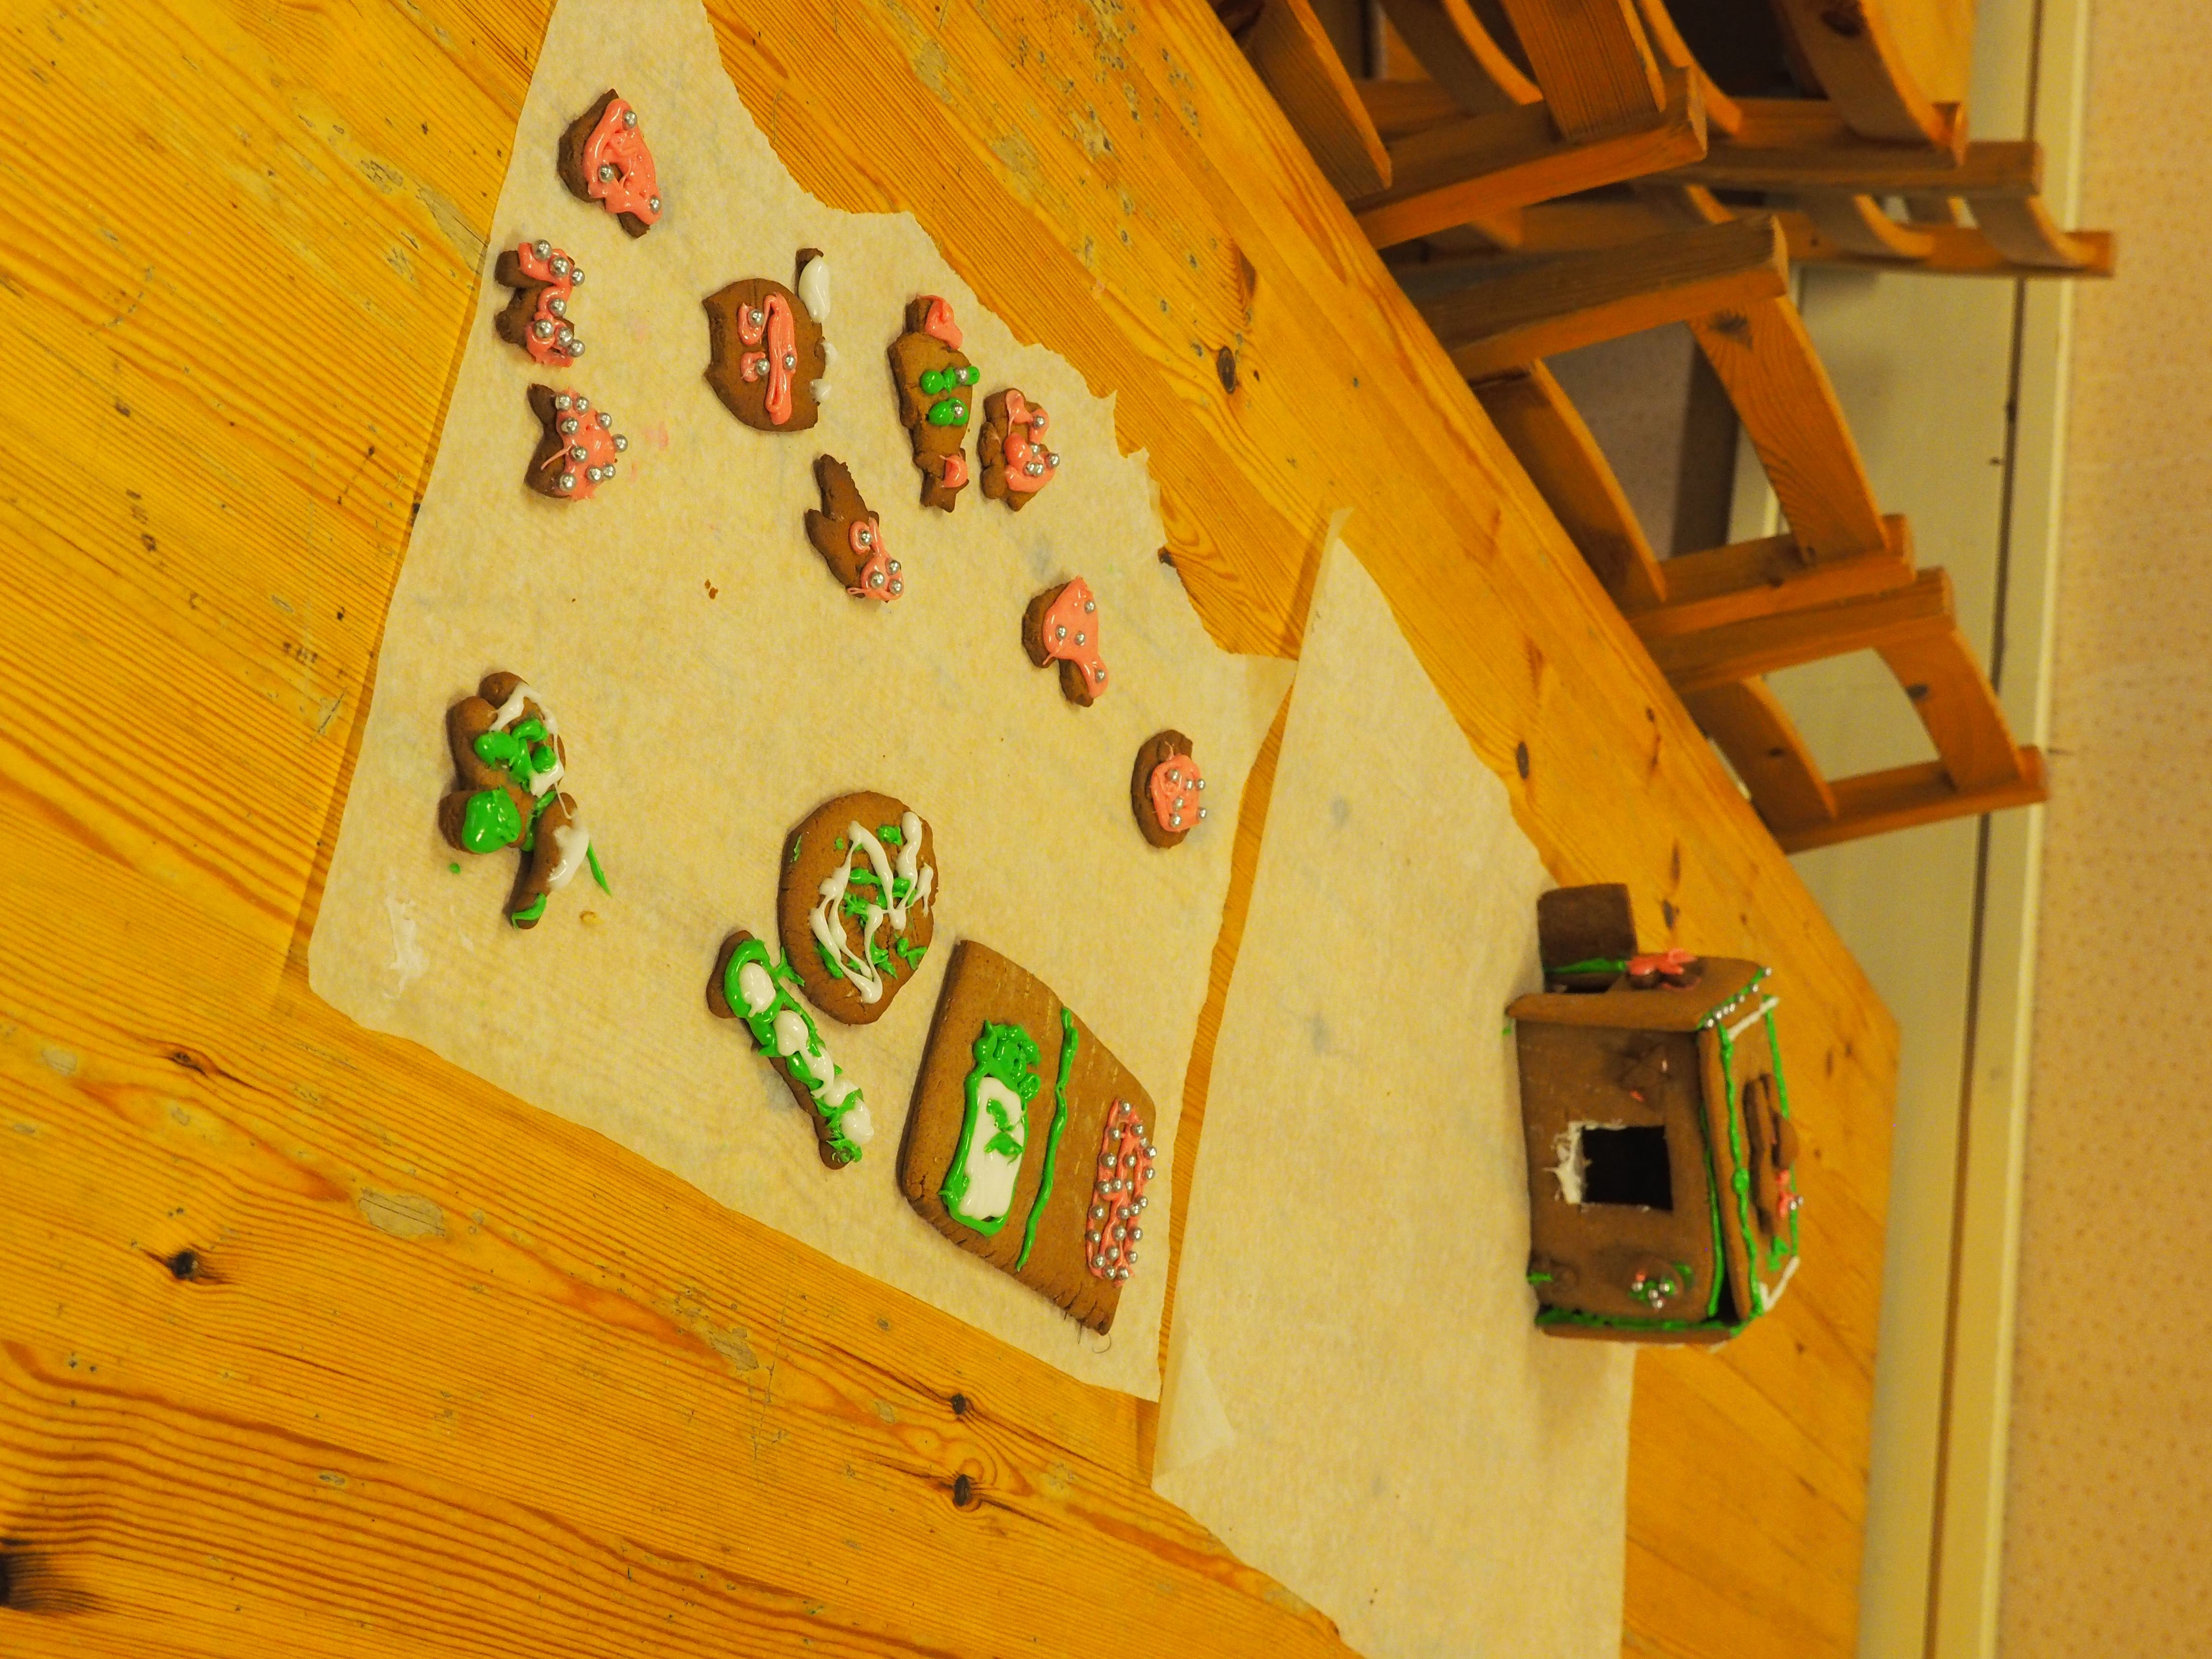
\includegraphics[width=.475\textwidth,height=.475\textwidth,keepaspectratio,angle=90]{assets/pipari2}

\vspace*{.05\textwidth}

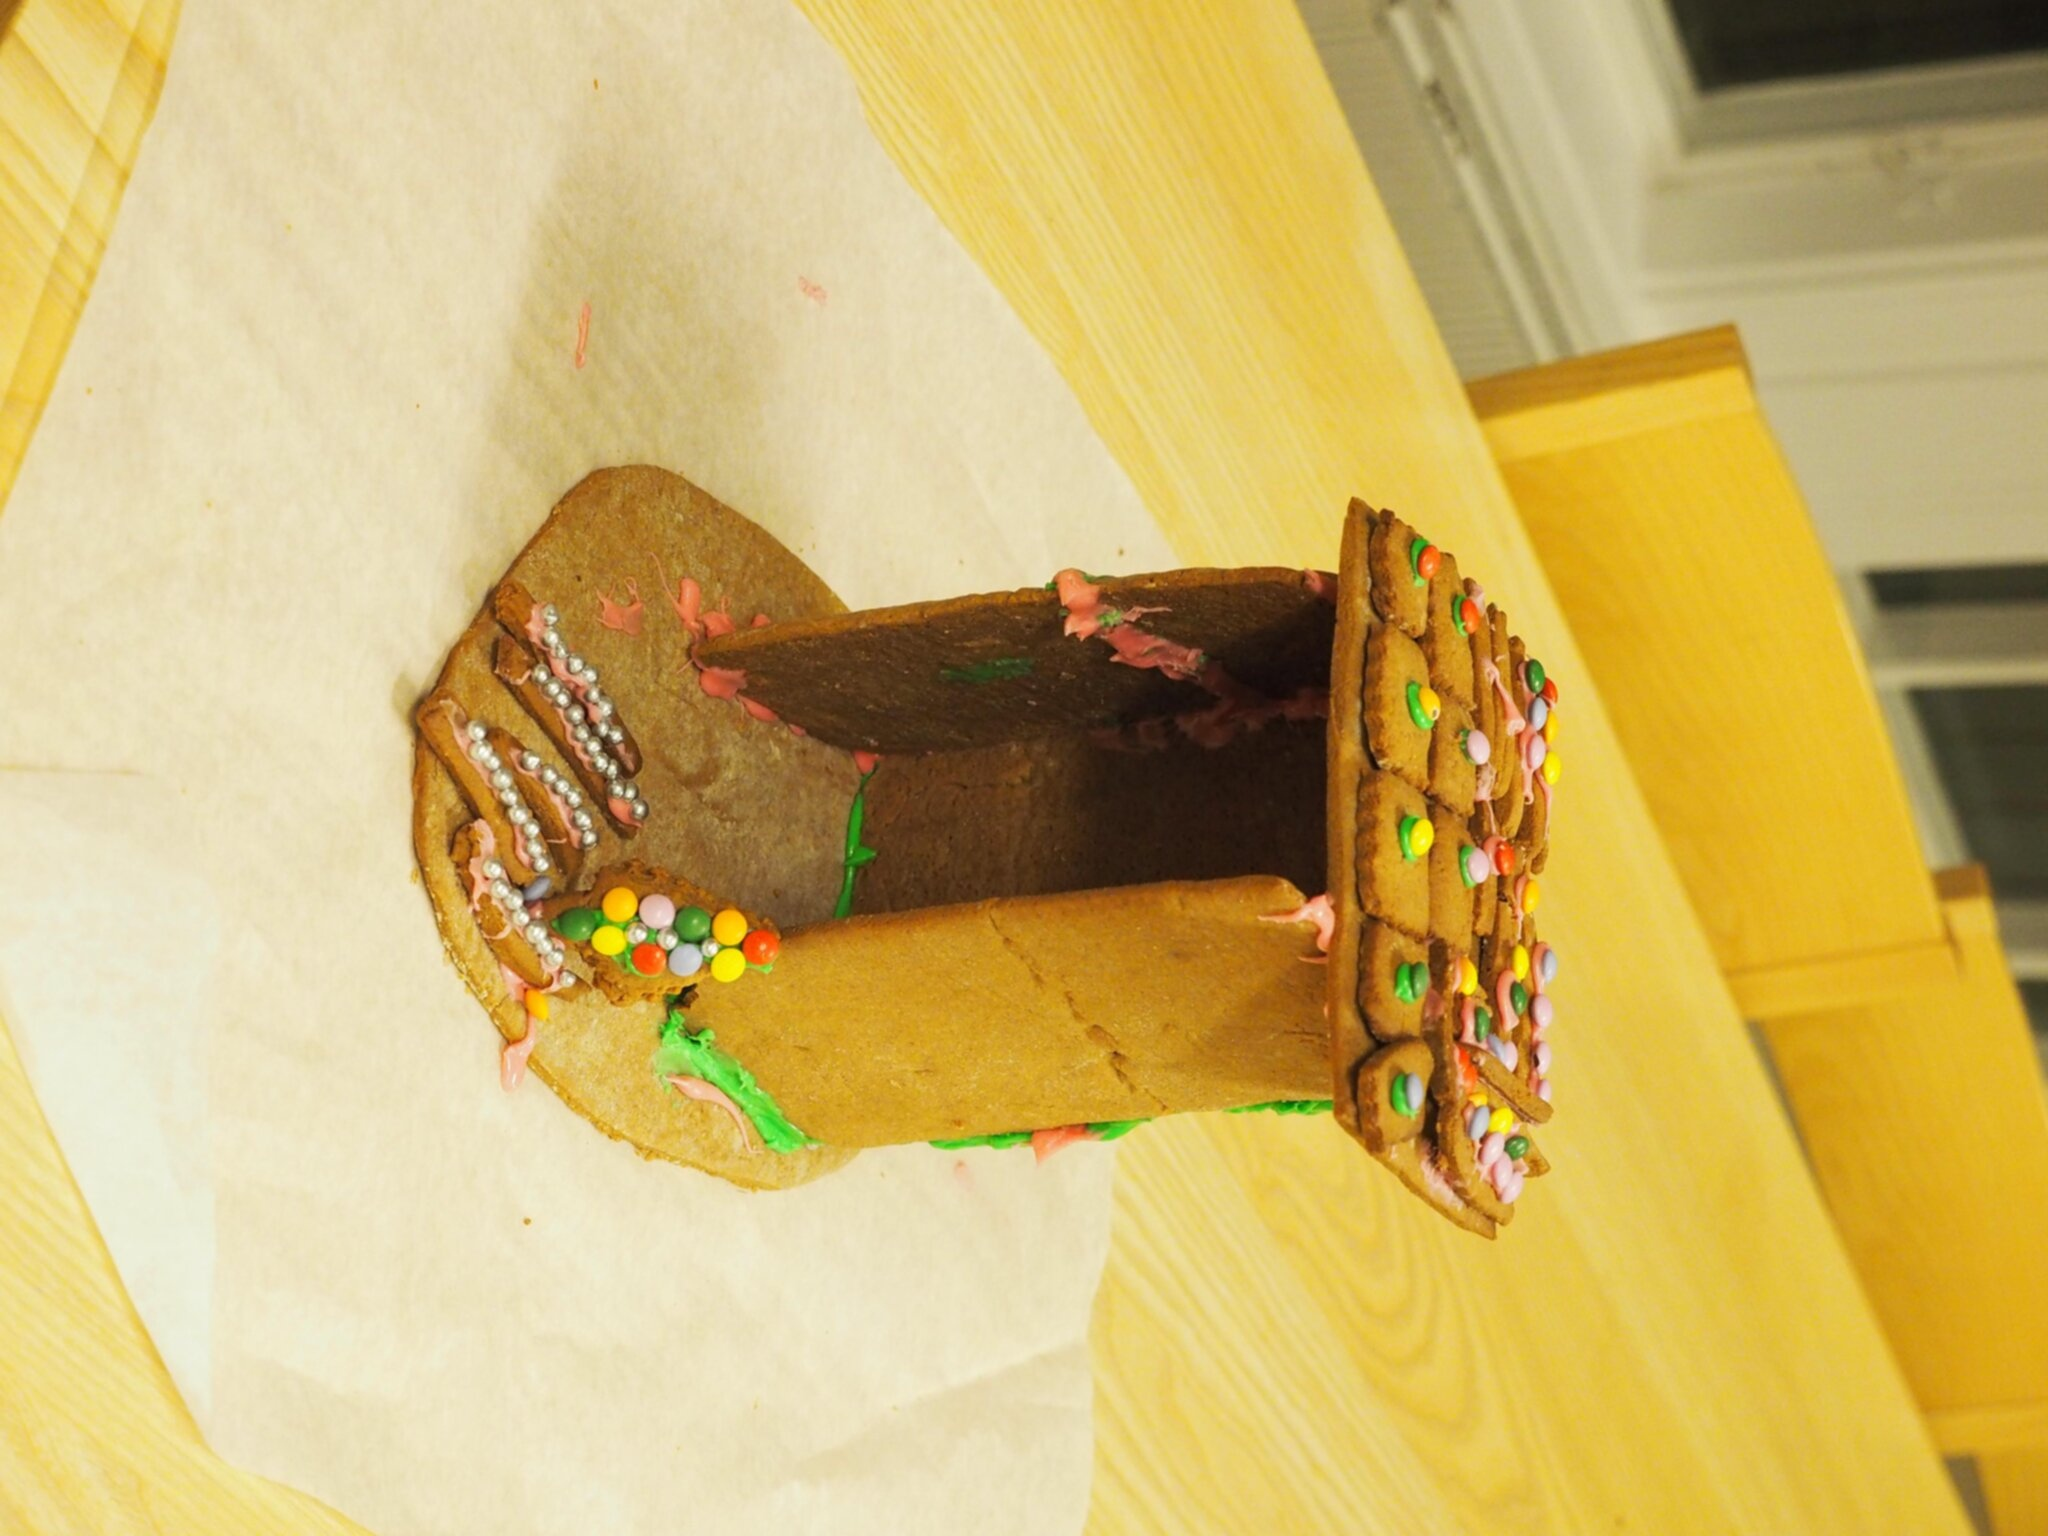
\includegraphics[width=.475\textwidth,height=.475\textwidth,keepaspectratio,angle=90]{assets/pipari4}\hfill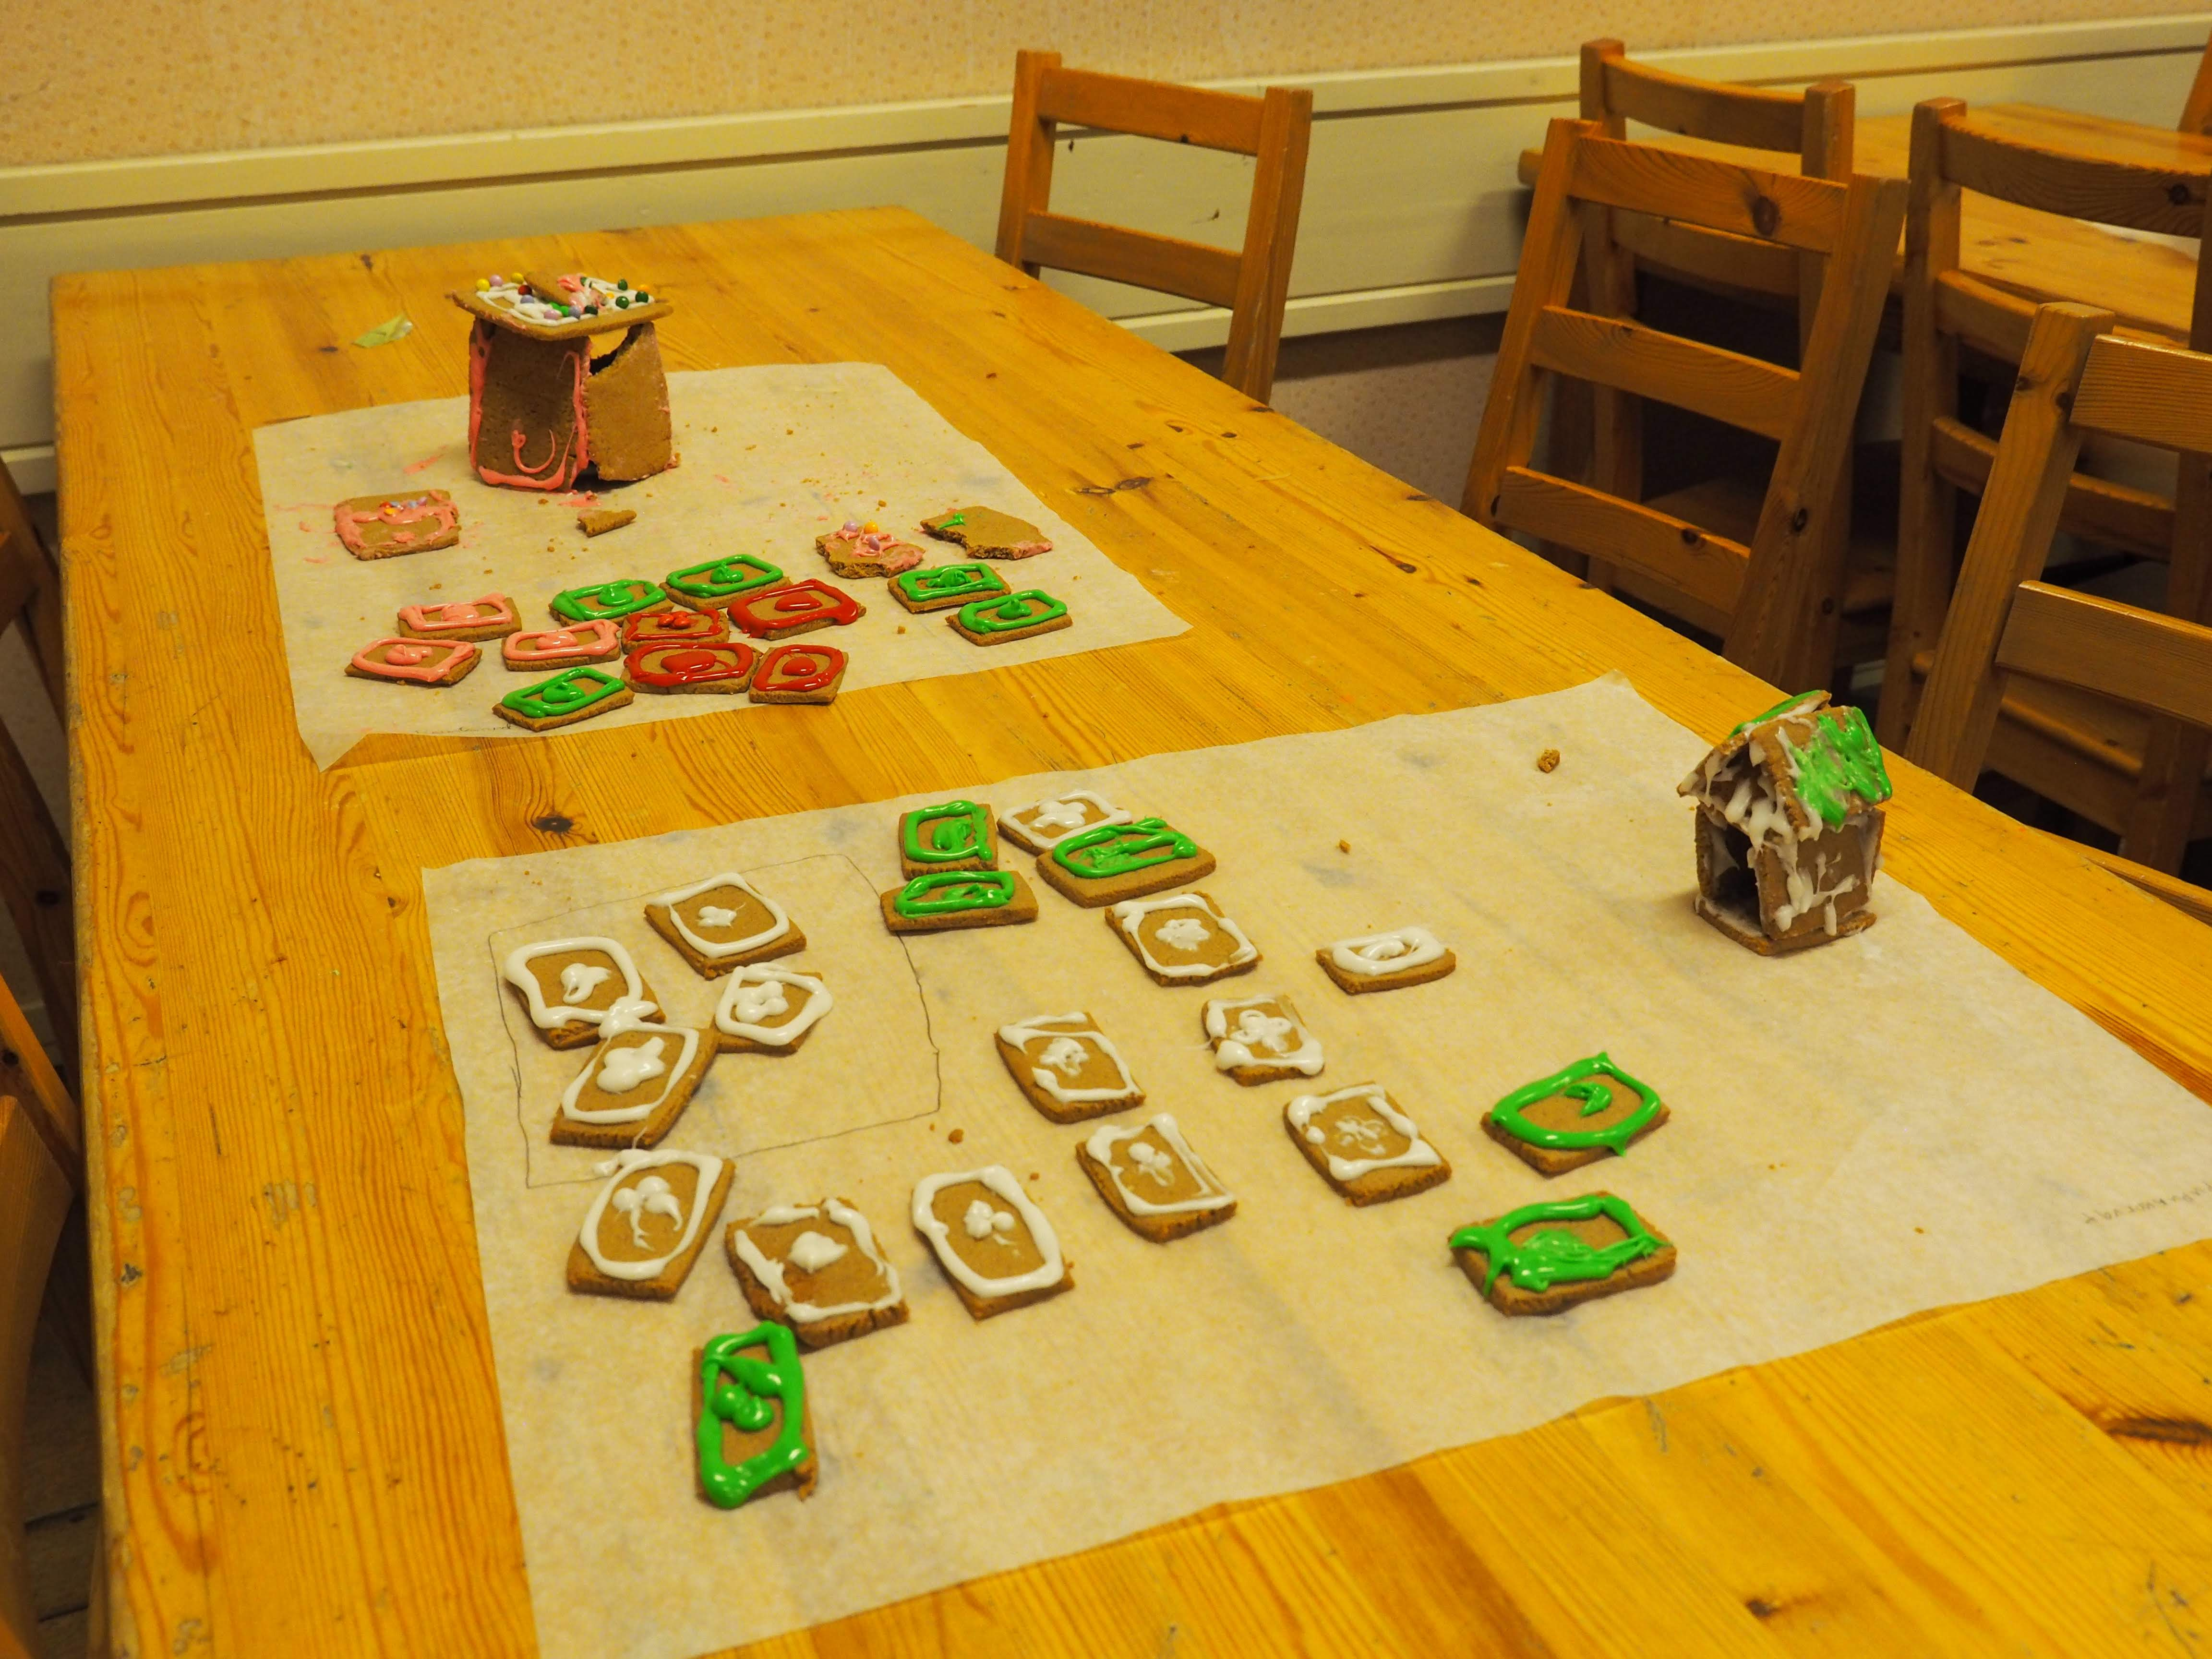
\includegraphics[width=.475\textwidth,height=.475\textwidth,keepaspectratio]{assets/pipari3}

\vspace*{.05\textwidth}

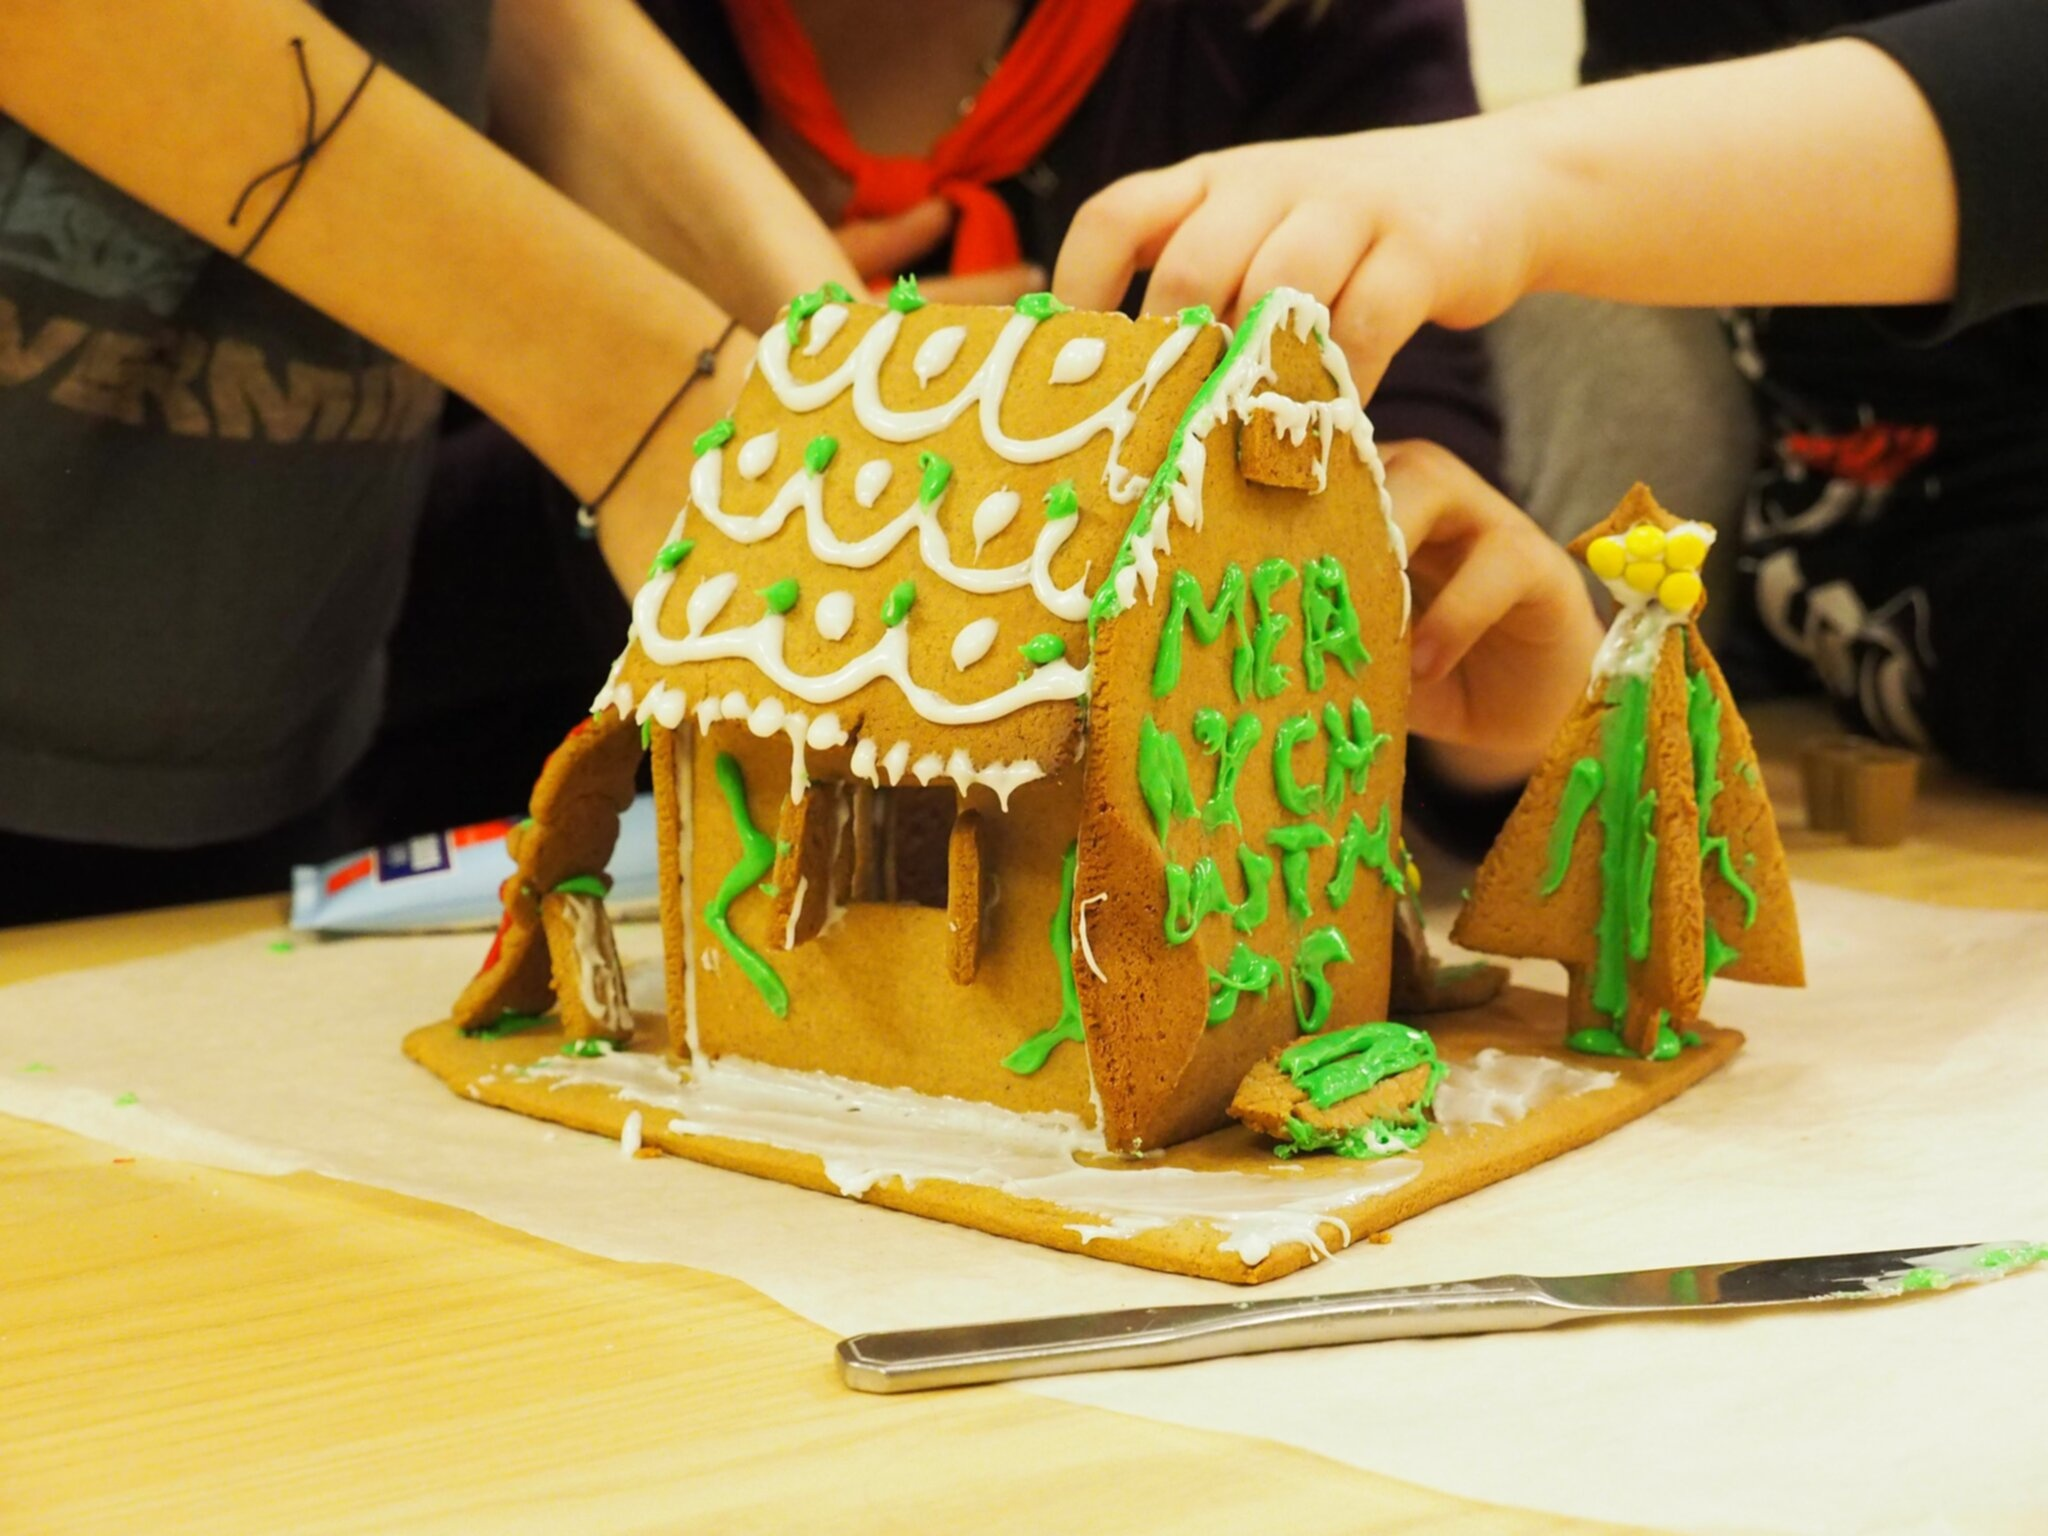
\includegraphics[width=.475\textwidth,height=.475\textwidth,keepaspectratio]{assets/pipari5}

\caption{Vartioiden piparkakkuteokset.}
\end{figure*}

Joulujuhlan juonsivat Tesla ja Touko ja se alkoi Päärynähyttysten 
spektaakkelimaisella näytelmällä joulupukista, tountuista ja nuuttipukista, 
joka huipentui joulupukin ja nuuttipukin eeppiseen räppäyskilpailuun! Listan 
joulujuhlassa ansioituneista löydät edellisestä Tassusta.

Juhlan päätyttyä luontotalo siivottiin loppuun ja lähdettiin kotimatkalle. 
Mitäköhän keksimmekään taas tämän vuoden pikkujouluretkelle?
\end{multicols}

\medskip

\noindent\null\hfill Kuvat: Janne ja Tanguy\\
\noindent\null\hfill Teksti: Janne

\section{Tarpojien minihaikki}


\noindent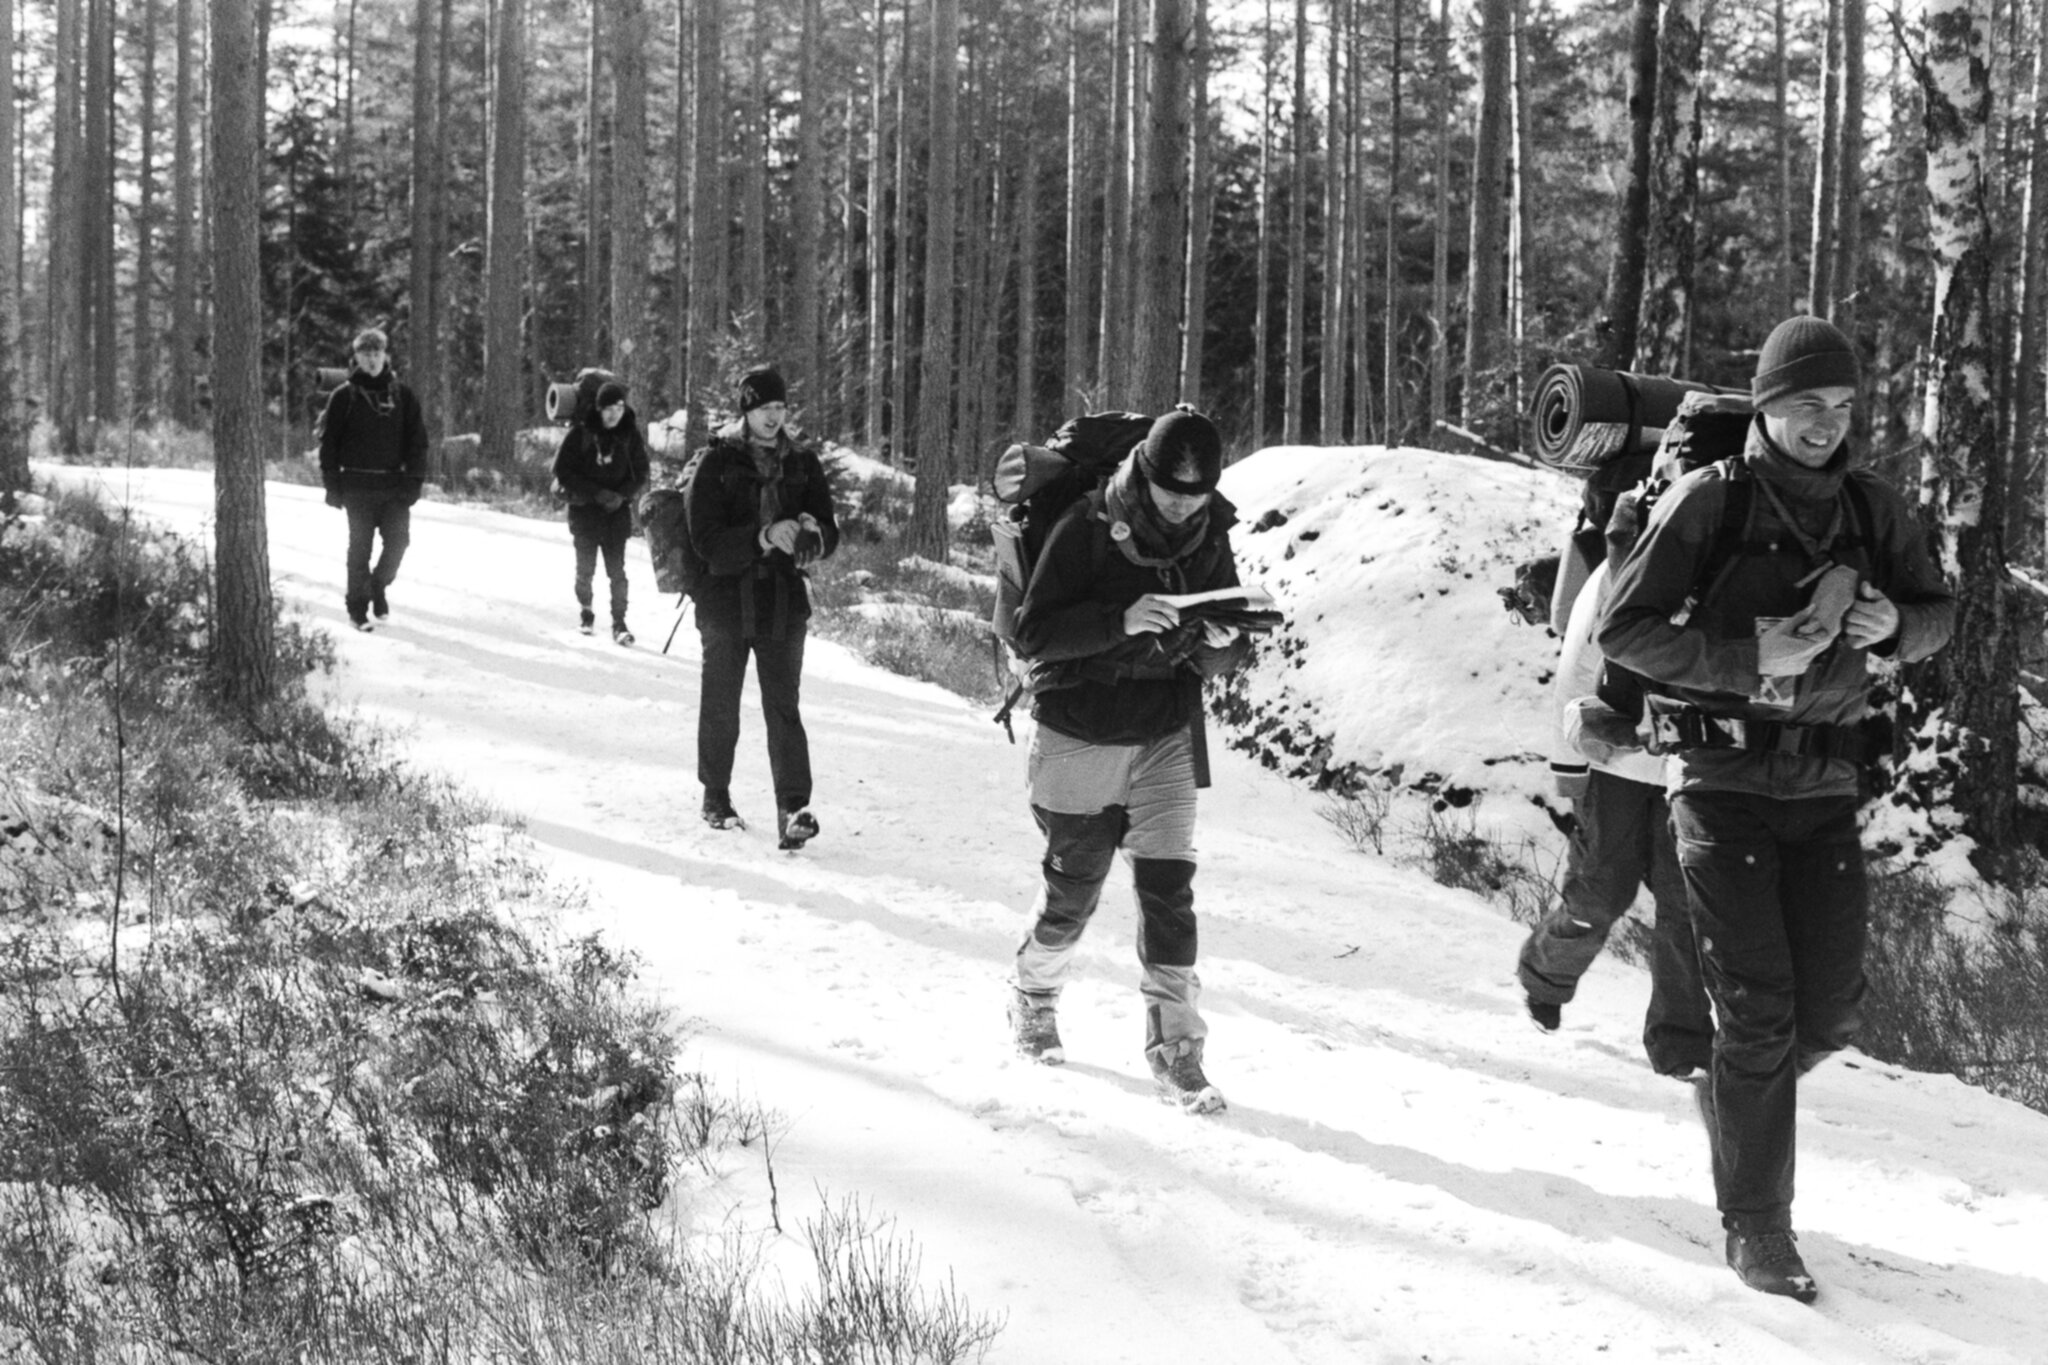
\includegraphics[width=1.0\linewidth,trim={0 0 0 1cm},clip]{assets/minihaikki4}

\begin{multicols}{2}

\noindent Perjantaina 14. maaliskuuta seitsemän rusakkoa lähti kohti Nuuksion
kansallispuistoa viettämään mukavaa viikonloppua pienimuotoisen vaelluksen
merkeissä. Vaikka vaellus oli nimensä mukaisesti tarpojille suunnattu, lopulta
matkaan lähti vain kolme tarpojaa, Alden, Jetro ja Tesla, sekä neljä johtajaa,
Ahti, Janne, Leo ja Tanguy. Retkikunta Leoa ja Jetroa lukuunottamatta lähti
liikkeelle kello 17.00 Kontulasta, Mikaelinkirkolta. Kontulasta hypättiin
metroon suuntana Rautatientori, josta matka jatkui E-junalla kohti Espoon
keskusta. Leo ja Jetro hyppäsivät junan kyytiin Huopalahden asemalta ja näin
koko retkikunta olikin kasassa! Junassa suoritettiin yhteisten varusteiden
jakoa, nautittiin matkaevästä ja manailtiin seuraavan yön sääennustetta, joka
lupaili jopa 9 asteen pakkasta. Onneksi kaikilla oli varusteet kunnossa,
jolloin kylmyys ei pääsisi haittaamaan! Junamatkan päätteeksi saavuttiin Espoon
keskukseen, josta bussi 245A lähti kuljettamaan retkeilijöitä kohti
kansallispuistoa. Bussimatka kesti kaikkiaan noin 20 minuuttia, minkä jälkeen
retkikunta jäi pois Kaitakorven bussipysäkillä. 

Ensimmäisen noin kahden kilometrin etapin suunnistamisen sai vastuulleen Jetro,
jonka tehtävänä oli suunnistaa porukka Hynkänlammen leiripaikalle. Reitti
Kaitakorvelta Hynkänlammelle kulki läpi Nuuksion ratsastuskeskuksen tilusten.
Hevosaitauksen vieressä kulkevaa polkua kävellessä retkikunnasta alkoi tuntua,
kun joku tuijottaisi heitä. Muutama ulkona oleileva hevonen ei selkeästi ollut
varautunut tunkeilijoihin, vaan tuijotti retkeilijöitä ihmeissään.
Hevoskohtaamisen jälkeen matka jatkui pienen nousun kautta ylös Hynkänlammen
keittokatokselle, joka oli retkikunnan ensimmäinen yöpaikka. Oli jo ilta ja
pimeää, minkä vuoksi retkikunta aloitti majoitteiden pystyttämisen miltei saman
tien. Kun muut lähtivät kasaamaan laavuja, telttaa tai riippumattoa, jäi Leo
tekemään tulia iltapalaa varten. Puut olivat kuitenkin märkiä eikä Leo
ymmärtänyt kasata nuotiota ylemmälle ritilälle tulipaikan pohjan sijaan,
jolloin tulen tekemisessä kesti odotettua kauemmin. Lopulta Ahti sai tulen
roihuamaan ja iltapalaksi nautittiin teetä ja makkaraa, minkä jälkeen väsynyt
retkikunta painui unten maille!

\vspace*{0.04cm}
\noindent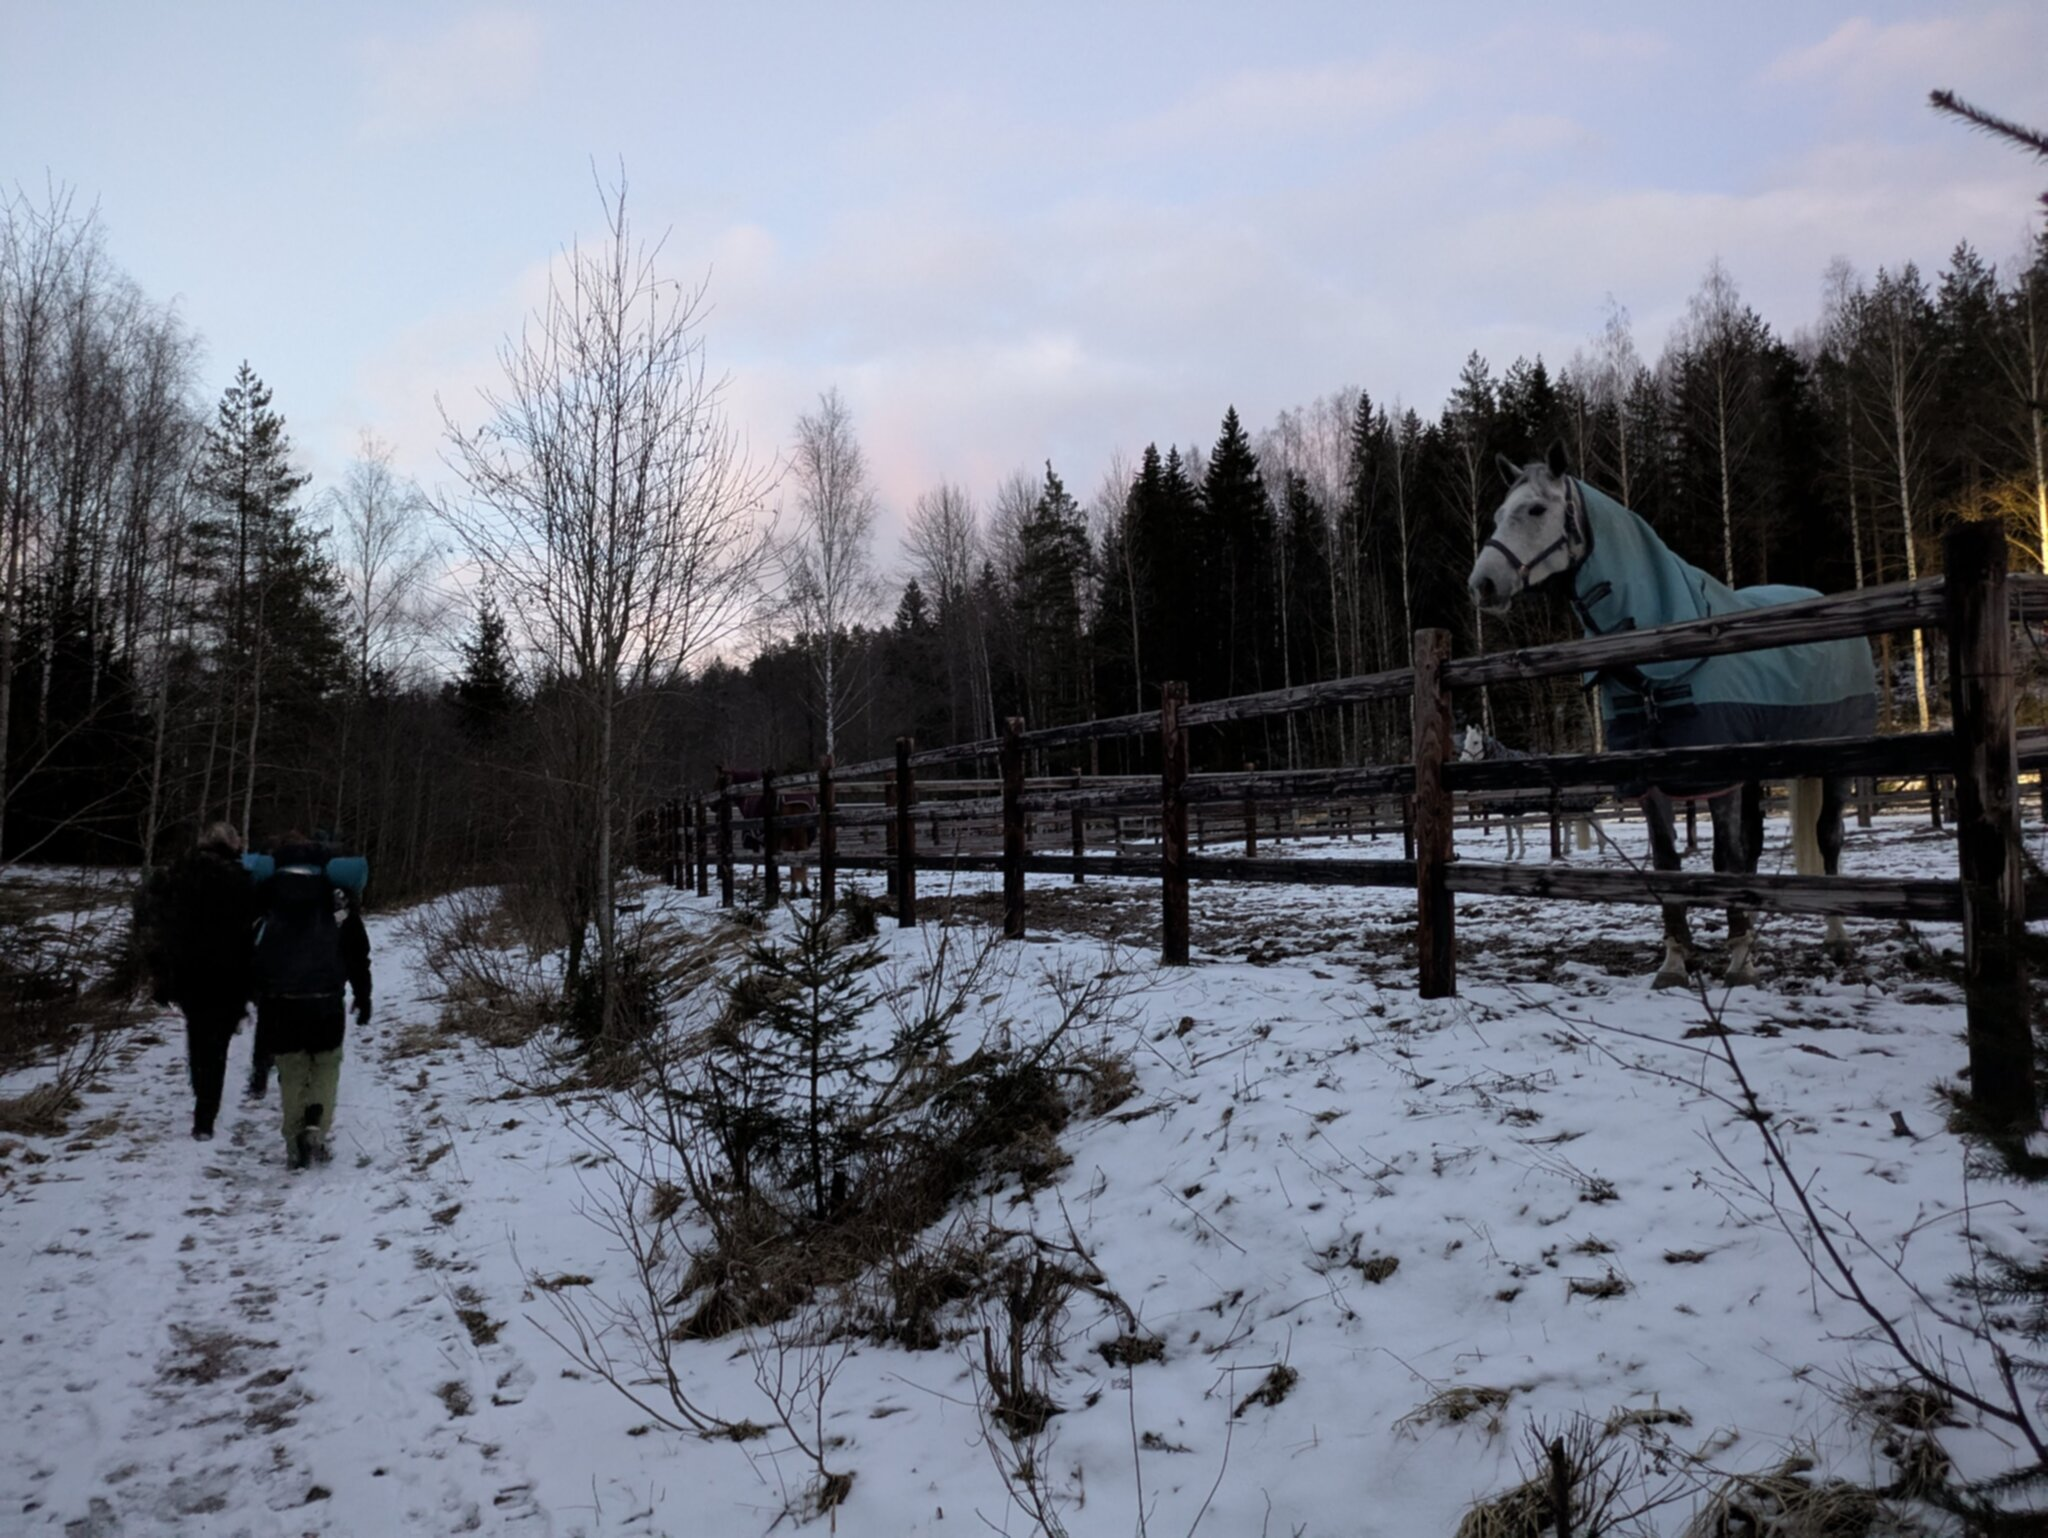
\includegraphics[width=1.0\linewidth,trim={0 10cm 0 10cm},clip]{assets/minihaikki1}

\vspace*{-0.32cm}
\noindent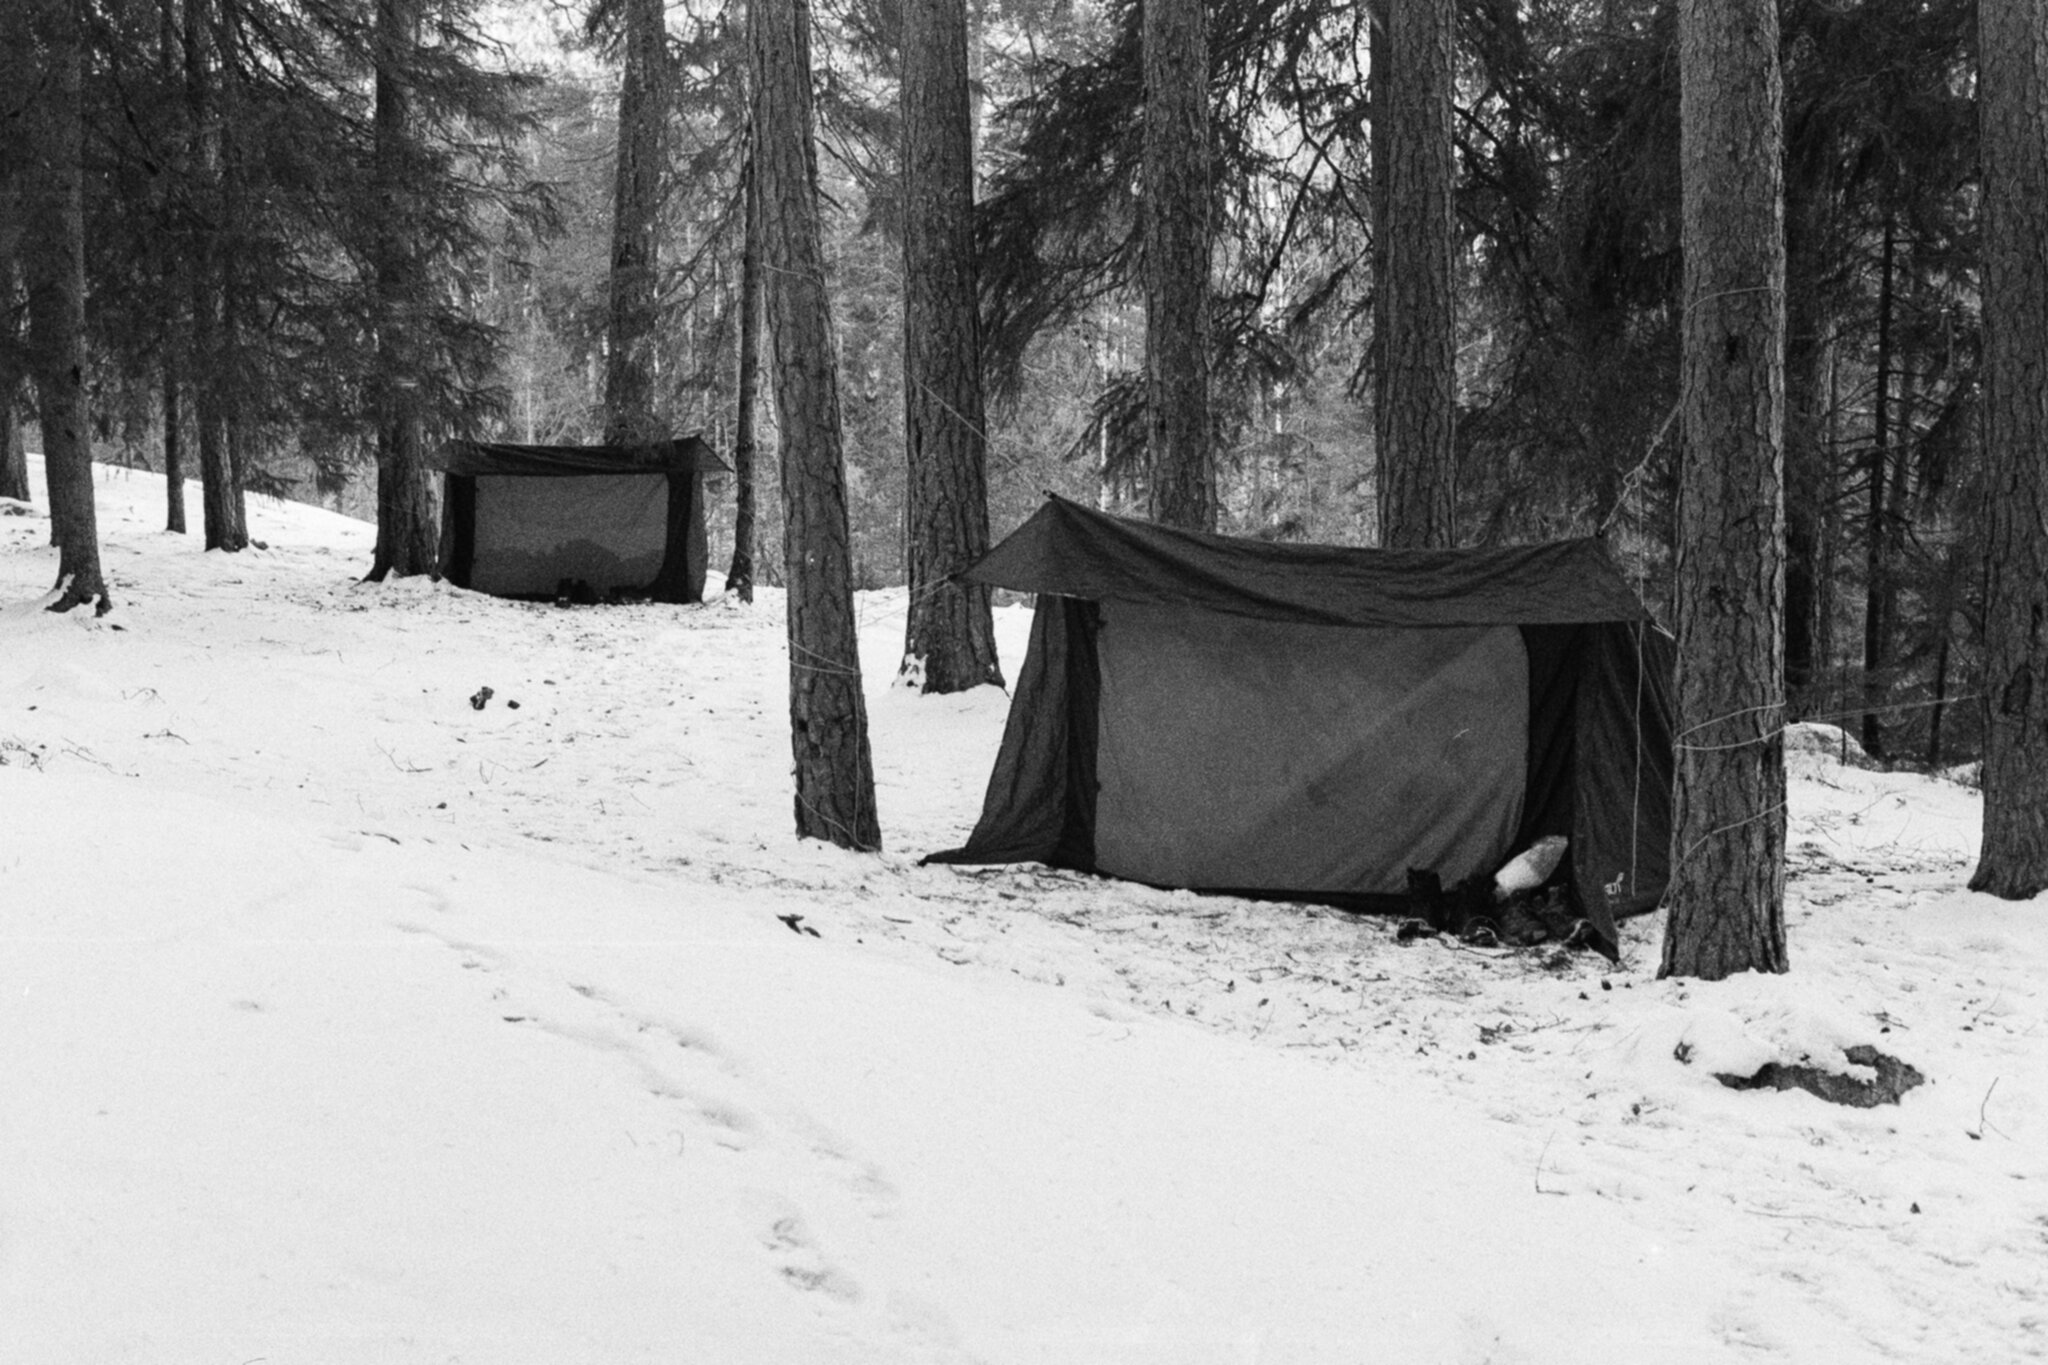
\includegraphics[width=1.0\linewidth,trim={0 2cm 0 2cm},clip]{assets/minihaikki2}

\noindent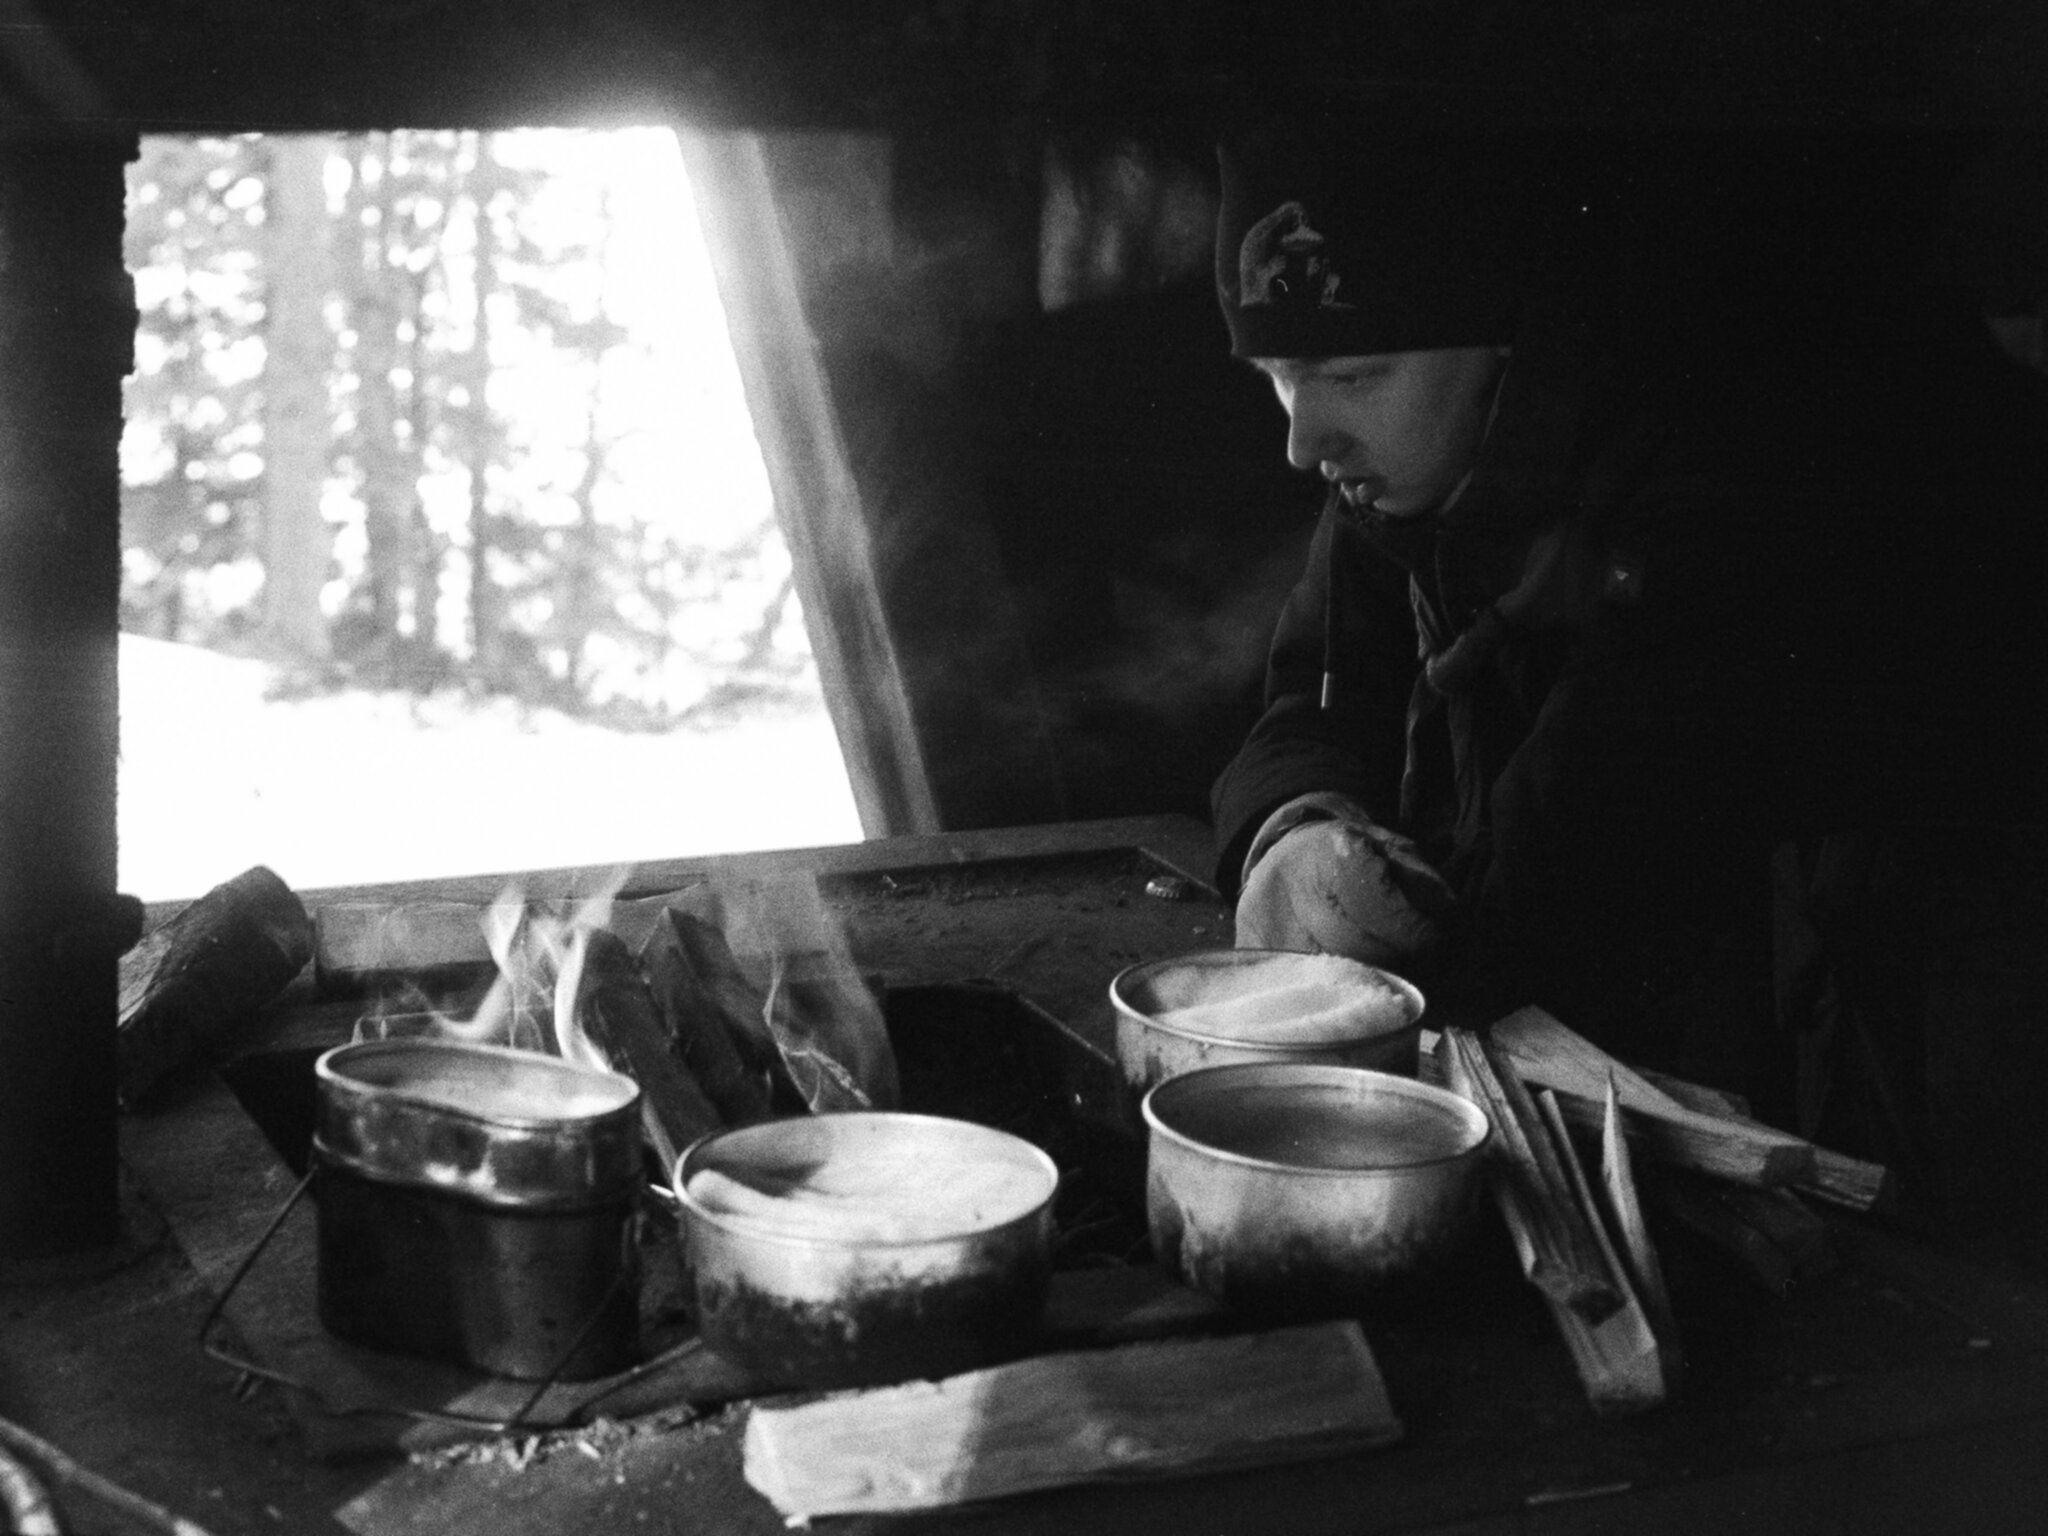
\includegraphics[width=1.0\linewidth,trim={0 0 0 0},clip]{assets/minihaikki3}

Aamulla herätessä todettiin, että sääennuste oli hyvinkin pitänyt paikkansa,
sillä ainakin allekirjoittanut voi todeta, että kylmyys tosiaan kiusasi. Yöllä
oltiin vältytty lumisateelta, mutta aamulla lämpötilan noustessa kosteus oli
hiipinyt sisään telttaan, jolloin varusteet olivat kostuneet. Aamupalalla
sitten kuivateltiin varusteita nuotion ääressä, puuroa, kahvia ja Oivallusta
nautiskellen. Pian olikin jo aika purkaa majoitteet ja jatkaa matkaa.
Ensimmäisen suunnistusvuoron sai Leo, joka pienen harhailun jälkeen sai
suunnistettua porukan lounaspaikalle. Noin kahden kilometrin kävelyn jälkeen
retkikunta pysähtyi Kattilajärventien varrelle valmistamaan lounasta.
Trangioilla valmistui herkullinen “ranskalainen” sipulikeitto, jonka mausteena
toimi kuivattu sipuli. Ja mitä olisikaan ateria ilman Oivallusta ja kahvia!
Lautaset tyhjinä ja energiaa täyteen tankattuina retkeilijät lähtivät tarpomaan
kohti seuraavaa etappia, Urja-järveä. Seuraavan suunnistusvuoron sai Alden,
joka sunnistikin onnistuneesti muutaman kilometrin matkan Urjalle, jonka
rannalla sijaitsikin jo seuraava yöpaikka. Matkalla päiviteltiin jälleen
seuraavan yön sääennustetta, joka vaikutti aiempaakin yötä karmeammalta. Yksi
aste lämmintä ja räntää…

\bigskip
\noindent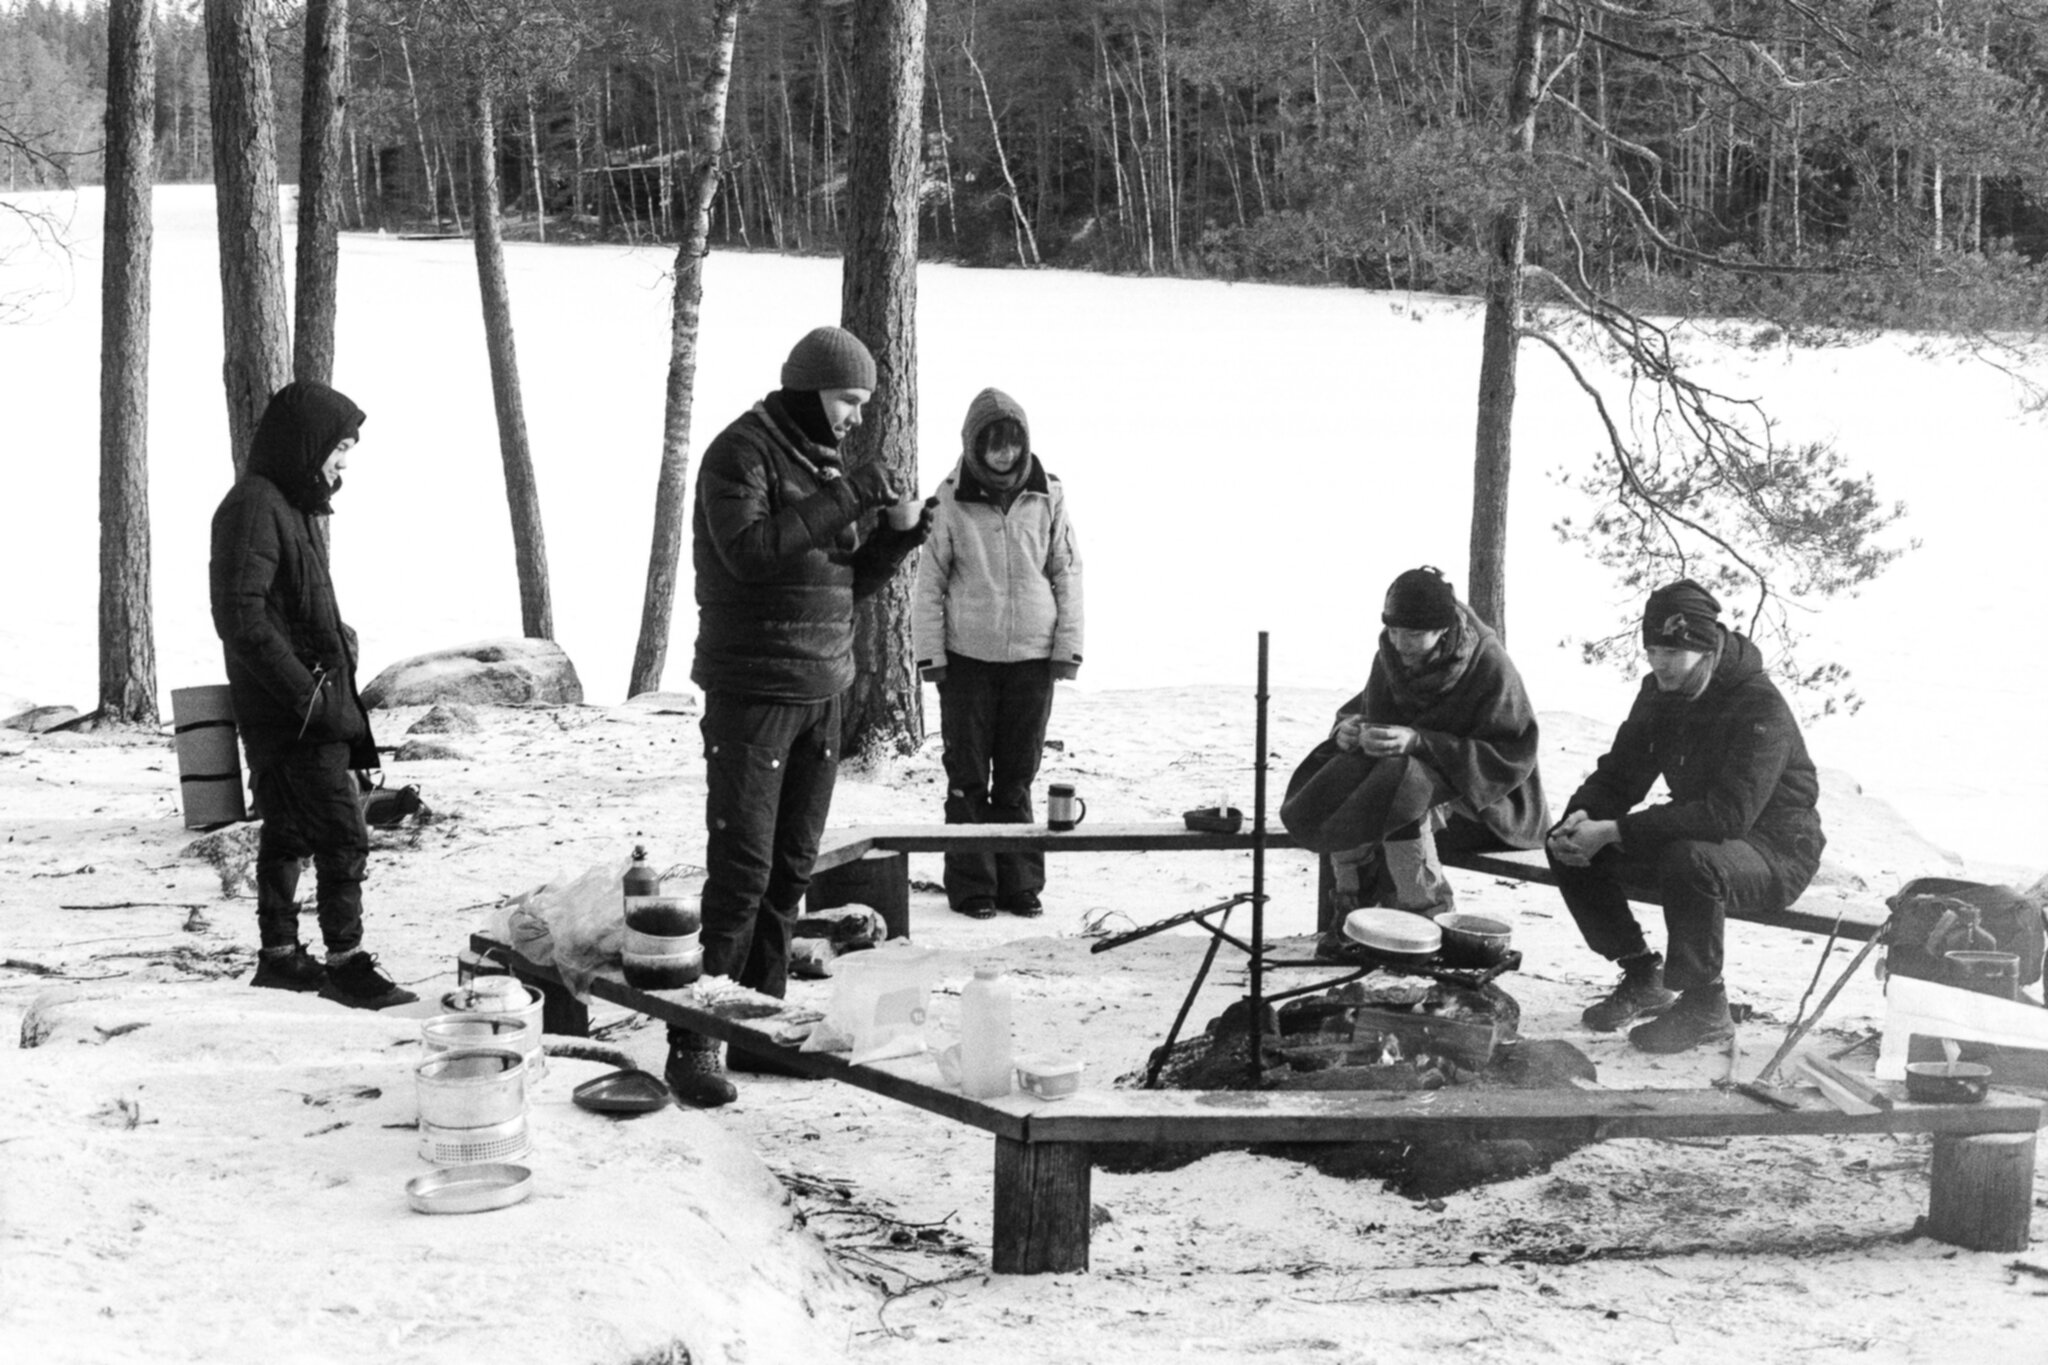
\includegraphics[width=1.0\linewidth,trim={0 0 0 0},clip]{assets/minihaikki6}
\smallskip

Urjalle saavuttaessa todettiin, ettei laavupaikan löytäminen ollut yhtään niin
helppoa kuin Hynkänlammella ja sopivia paikkoja etsittiin miltei puoli tuntia.
Kun paikat löytyivät ja majoitteet saatiin kasaan, oli jälleen ruoka-aika.
Koska Urjalla oli rusakoiden lisäksi muitakin retkeilijöitä, jotka olivat
miehittäneet nuotiopaikan, täytyi retkikunnan valmistaa ruokaa trangialla.
Iltaruuaksi syötiin tomaattista soijapataa sekä salami-tomaattipastaa.
Kasvisruokailijoiden harmiksi soijanpalaset maistuivat pitkälti pahvilta, mutta
siitä huolimatta vatsat saatiin täyteen. Loppuilta kuluikin yhdessä aikaa
viettäessä ja jutellessa. Iltapalana oli Hönöä, Oivallusta, Lämmintä kuppia ja
teetä. Illan pimentyessä ja kylmetessä retkikunta painui nukkumaan.

\vfill\null
\columnbreak

\begin{center}
\noindent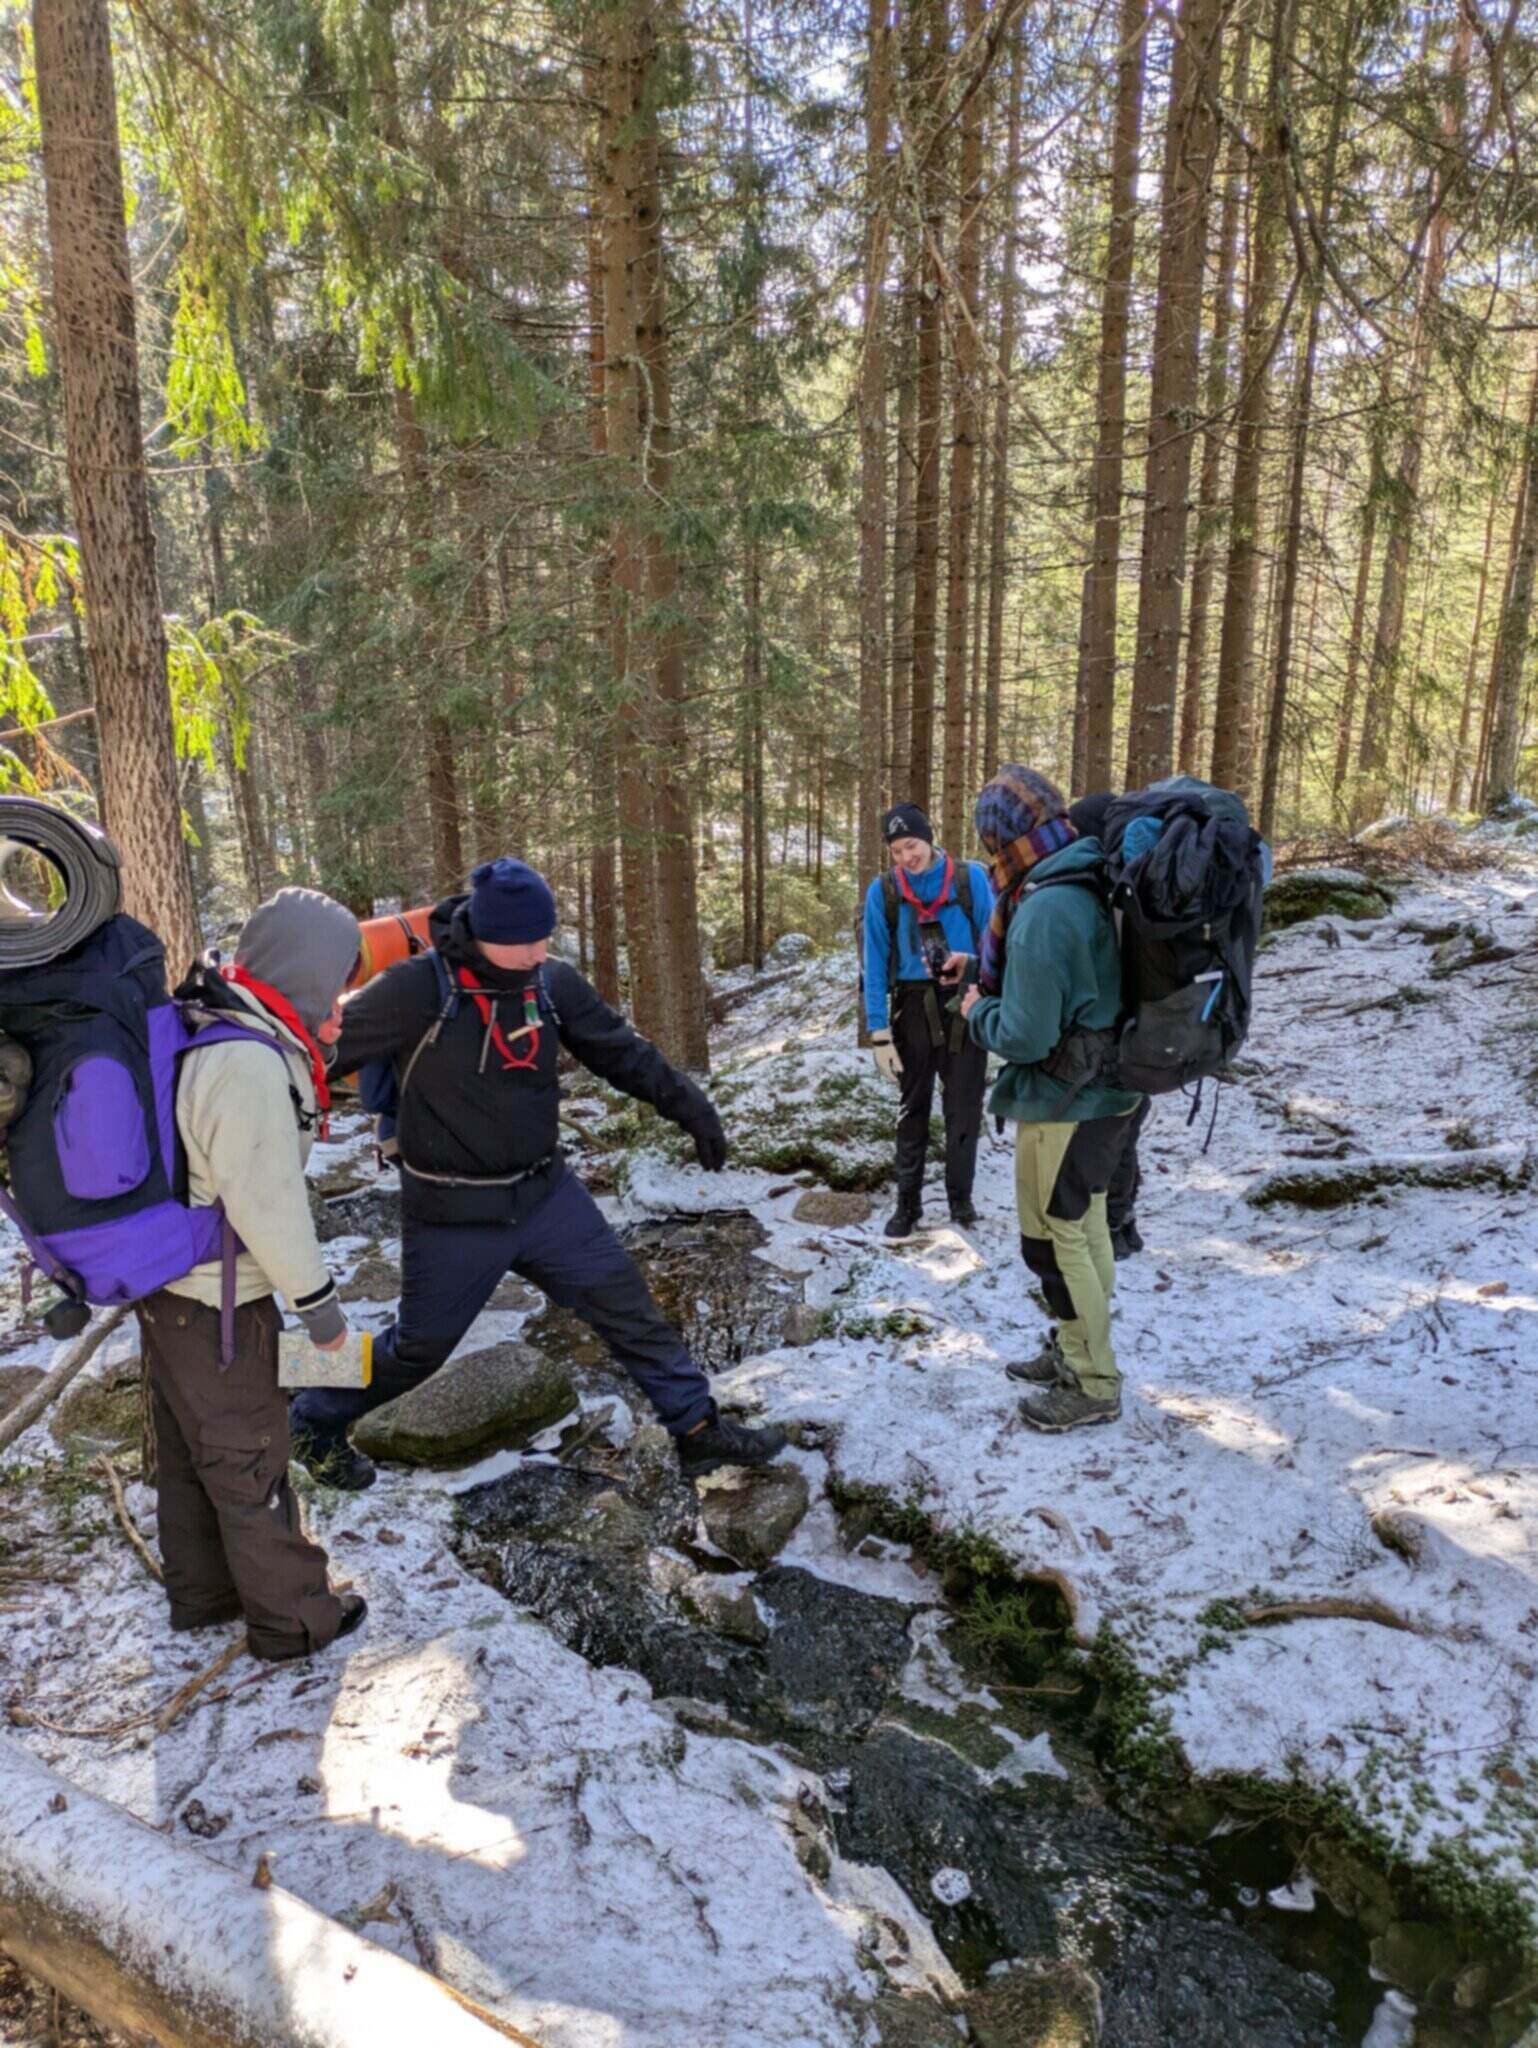
\includegraphics[width=1.0\linewidth,trim={0 0 0 0},clip]{assets/minihaikki5}
\end{center}

Haikin viimeinen aamu alkoi kosteissa tunnelmissa. Sääennuste oli totta tosiaan
pitänyt paikkansa ja yön räntäsade oli tullut läpi laavun katosta. Etenkin
teltan keskiosaan kerätyt tavarat kuten allekirjoittaneen toppatakki olivat
kastuneet. Onneksi muulta seurueelta sai kuivaa vaatetta lainaan, minkä lisäksi
aamupuuro ja -kahvi sekä nuotio lämmittivät aamun kylmyydessä. Aamiaisen
jälkeen oli vielä aika tiskata astiat, pakata loput tavarat ja purkaa
majoitteet, minkä jälkeen matka pääsi jatkumaan. Suunnistusvuoron sai nyt
puolestaan Tesla, jonka tehtävänä oli suunnistaa seurue Haltiaan
bussipysäkille. Matkalla päädyttiin kuitenkin tekemään pieni poikkeus, kun
retkikunta päätti lähteä katsomaan Meerlammen luolaa. Matkalla luolalle
ylitettiin pieniä vesialueita, listattiin suomen kielen mö-alkuisia sanoja ja
nautittiin auringonpaisteesta, jota oli kaivattu koko viikonlopun ajan.

Meerlammella todettiin, että “luola” on hiukan harhaanjohtava termi paikalla
olevista kallioista ja suurista siirtolohkareista. Se oli kuitenkin mukava
levähdyspaikka ja sen kivimuodostelman alla saatiin otettua myös retken
virallinen yhteiskuva. Meerlammen nähtävyyksien jälkeen matka jatkui kohti
Haltiaa. Matkalla aloitettiin jälleen uusi kielellinen haaste, kun retkikunta
alkoi keksimään tulevan kesän vaellukselle v-kirjaimella alkavia nimiä.
Juomaveden loppuessa osa alkoi maistella Nuuksion purojen virtavesien
tarjontaa, mikä herätti muissa hiukan ihmetystä. Lopulta saavuttiin Haltiaan,
jolloin todettiin koko minihaikin matkasaldoksi yksitoista kilometriä.
245A-bussia saatiin odotella jonkin aikaa, jolloin oli hyvin aikaa käydä vielä
vessassa Haltian luontokeskuksessa. Bussimatka saatiin jakaa kahden muun
Nuuksiossa retkeilleen lippukunnan kanssa tupaten täydessä bussissa. Espoon
keskuksesta lähdettiin E-junalla kohti kotia. Ikävistä sääolosuhteista
huolimatta retki oli onnistunut ja seurue jälleen valmiina uusiin
seikkailuihin.
\columnbreak

\noindent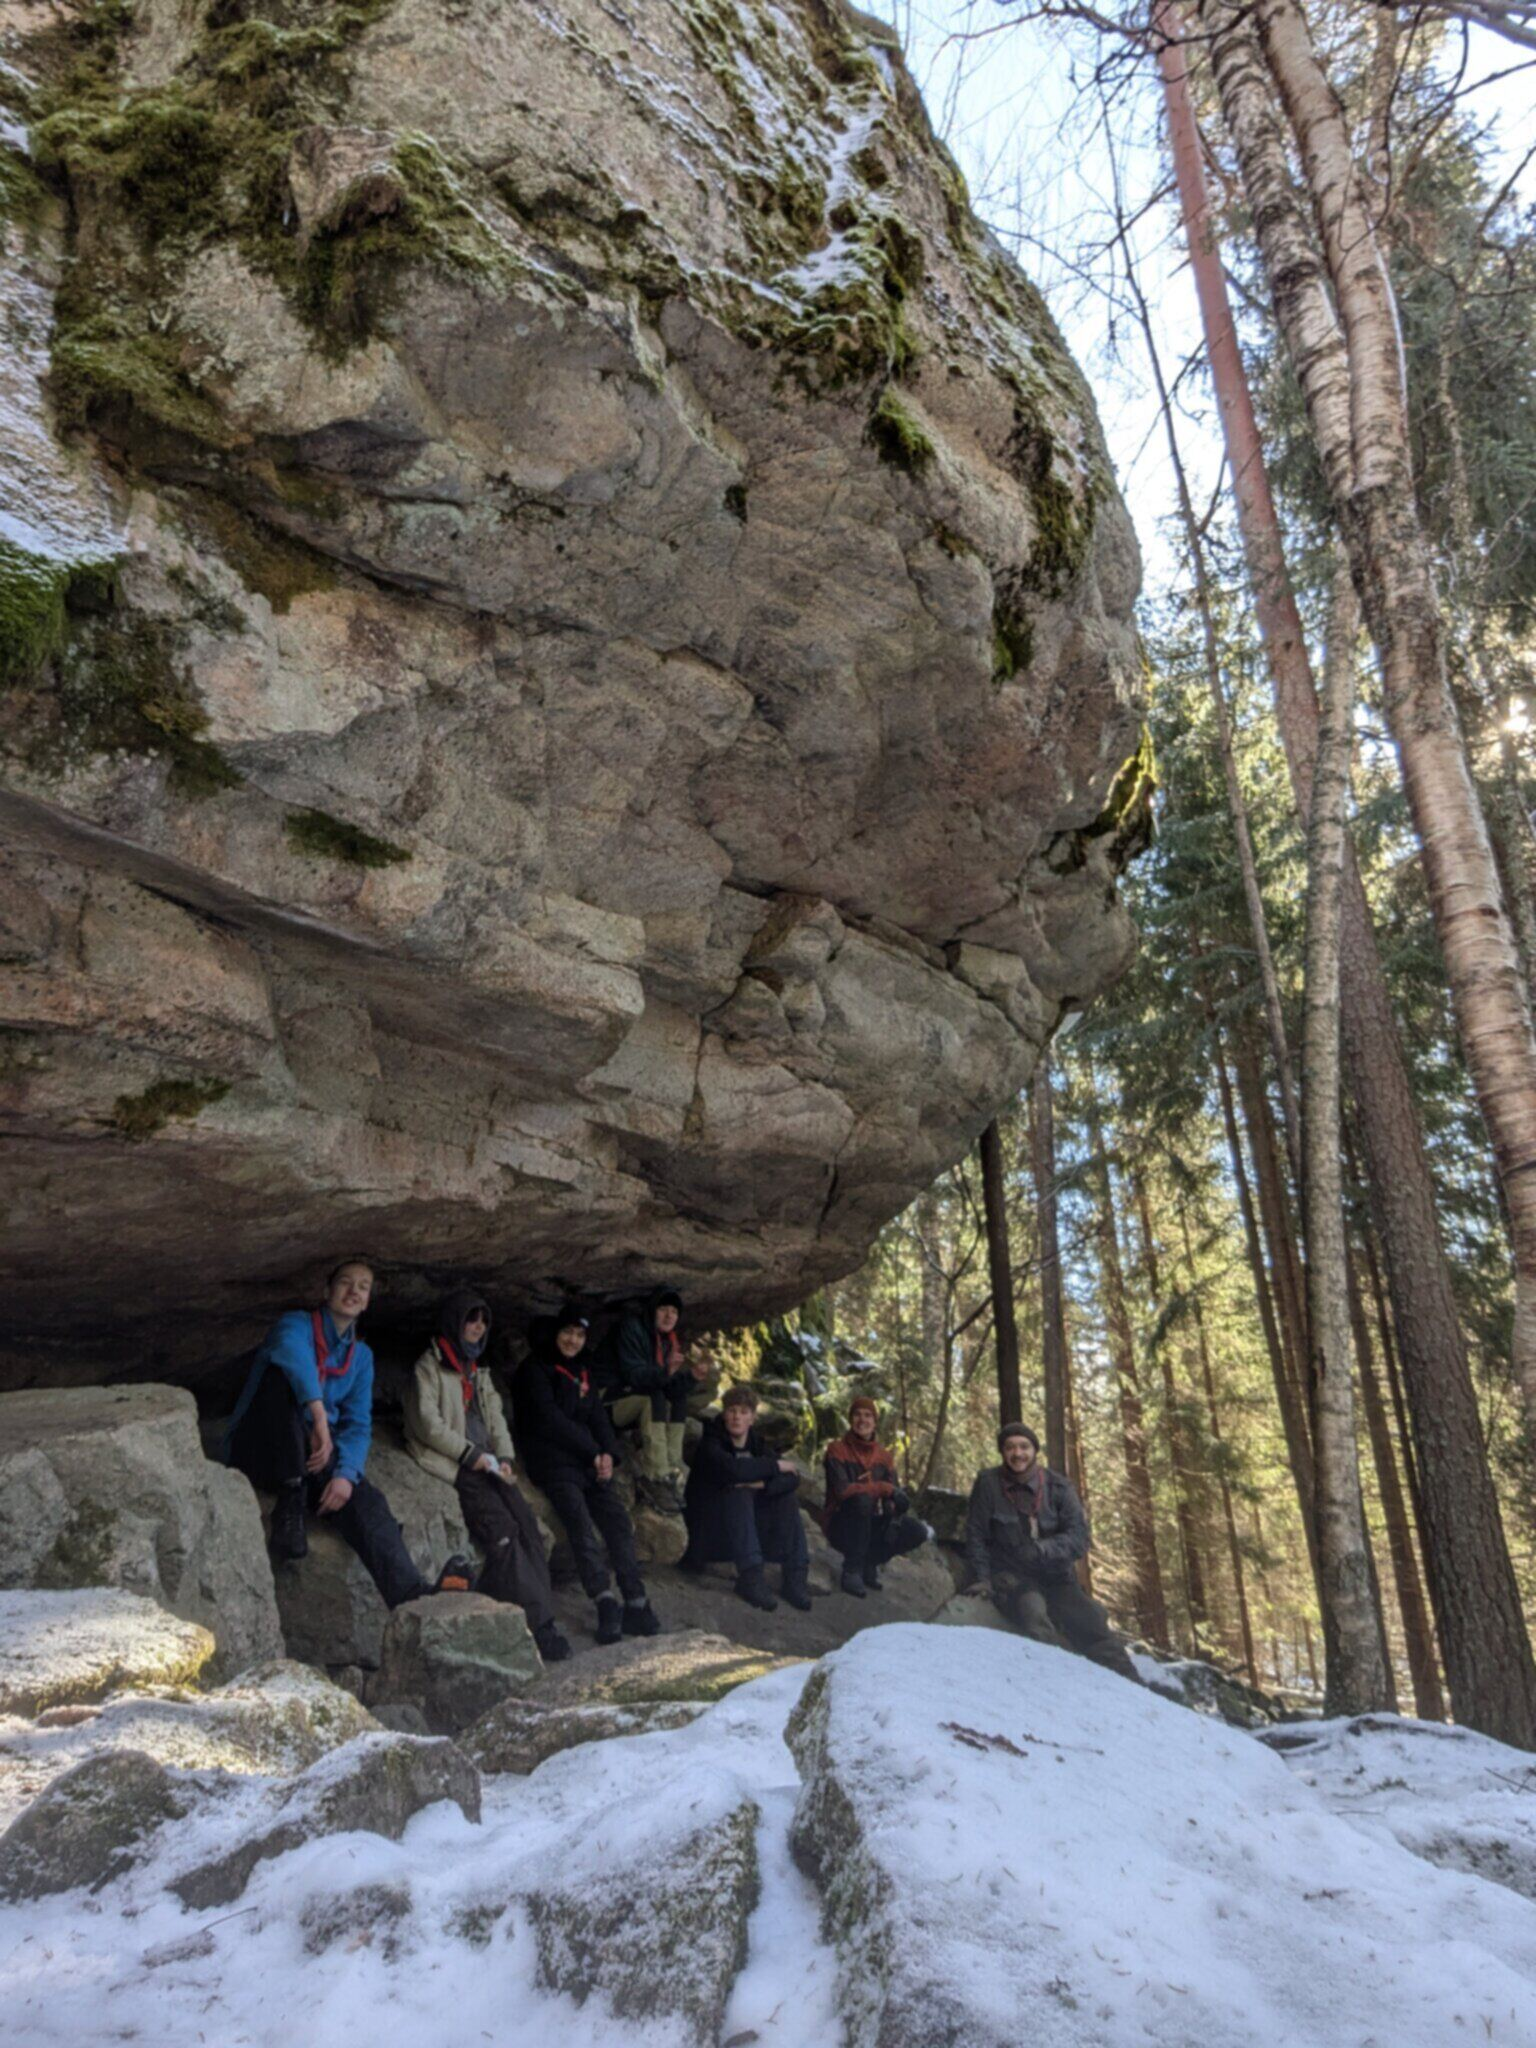
\includegraphics[width=1.2\linewidth,trim={4cm 0 6cm 0},clip]{assets/minihaikki7}

\end{multicols}


\vspace{1cm}
\noindent\null\hfill Kuvat: Tanguy\\
\noindent\null\hfill Teksti: Leo

\section{Riihitykset Piilopirtillä KESKEN}

\textit{Rusakoiden vanhempien ikäkausien yhä seuraamat 
luokkamerkkivaatimukset ovat lippukunnan oma sovellus perinteisistä 
suomalaisista partio"-ohjelmista. Luokkamerkkien avulla opitaan monia 
hyödyllisiä erätaitoja ja tutustutaan partiotapoihin. Luokkamerkin 
loppukokeessa eli riihityksessä päästään soveltamaan opittuja taitoja 
käytännössä.}

\textit{Viimeksi riihityksiä on järjestetty Sipoonkorvessa 12.2.2025, 
Länsi"-Helsingissä 9.6.2019 ja Nuuksiossa 10.2.2018. Tässä jutussa 
päästään kurkistamaan niin sanotusti esiripun taakse, kun julkaisemme 
vuoden 2018 riihityksenaikaisen rastimiesten Whatsapp"-ryhmän keskustelun. 
A"-Team"-vartio teki Lentävä nuoli "=merkkiin liittyviä rastitehtäviä, kun 
taas Jamalit 5000 ja Suunnistajat"-vartiot suorittivat III luokkaa ja 
Unibrows"-vartio II luokkaa. Julkaisemme myös Unibrows"-vartion kirjoittaman 
riihitysraportin ensimmäistä kertaa.}

\medskip

\noindent\null\hfill Kuva ja teksti: Janne

\begin{multicols}{2}
\setlength{\parindent}{0em} 10.59 - V: A-team matkalla! (J: ilmoita myös 
kumpaa puolta Orajärveä 2:lta lähdetään)

11.02 - V: Jamalit 5000 lähtee, tai ainakin kovasti yrittää...

11.04 - V: Suunnistajat lähtee

11.08 - V: Ja viimeisetkin matkaan!

11.29 - T: Rastimies 1 asemissa, ryhmästä X näkö- ja äänihavainto 
toiselta rannalta

11.46 - J: Rastimies 2 matkalla: etappi 1-2 erit. raskas. ~30 cm lunta, ei 
tallottu...

11.48 - T: Ryhmä 1 poistui rastilta 2

11.51 - J: Suunnistajat hukassa. Soittivat. Ovat ilmeisesti Ruuhijärven 
rannassa...

11.52 - T: Taisivat minulle koittaa kanssa, en ehtinyt vastata. Muut 
rastilla/matkalla rastille 2

12.08 - J: Rasti 2 asemissa.

12.12 - V: Rastia 4 vielä etsitään, eli 3:lle ei kannata ketään 
päästää...

12.19 - T: Viimeinen ryhmä saapui rastille 1, vahvuus vain 3, yksi puuttuu

12.22 - T: Ryhmä siis suunnistajat, K ilmeisesti palannut kämpälle, tai 
ainakin sinne suuntaan lähtenyt

12.33 - T: Viimeinen ryhmä poistui rastilta 1, rastimies aloittaa siirtymän 
kohti rastia 5

12.36 - J: Onko rasti 3 asemissa?

12.36 - V: Ei, vielä ei edes 4 löytynyt...

12.38 - J: A-Team lähtövalmiudessa rastilla 2. Odottaa lähtölupaa...

12.46 - M: Rasti 4 on miehitetty. Täällä on korppi!

12.51 - J: Jamalit 5000 lähtövalmiudessa rastilla 2. Odottaa lähtölupaa...

13.05 - J: Unibrows lähtövalmiudessa rastilla 2. Odottaa lähtölupaa...

\begin{figure*}[!t]
\centering\small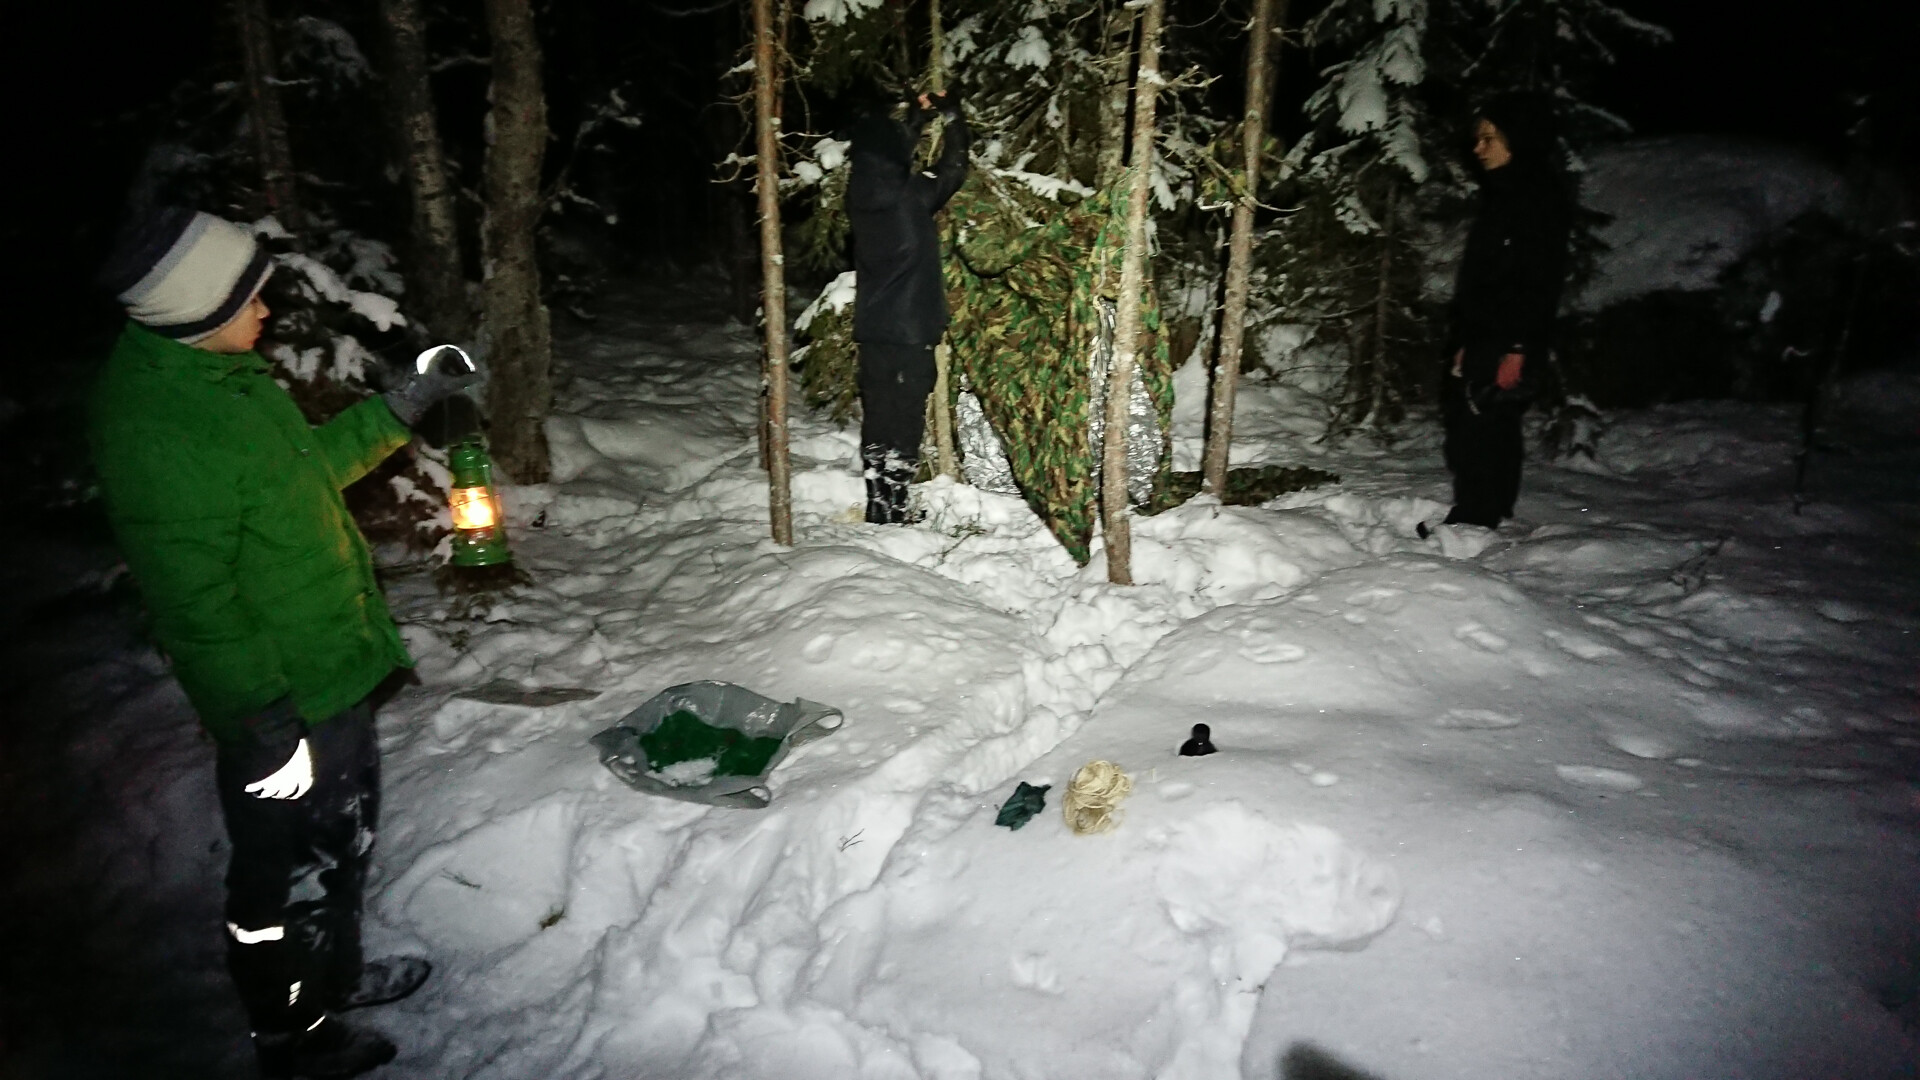
\includegraphics[width=\textwidth]{assets/riihitys2018}
Unibrows"-vartio riihityksen viimeisellä rastilla kasaamassa myrskylyhtyä ja 
laavua.
\end{figure*}

13.09 - T: Ruokarastille saavuttu, eksynyt lammas seisoi kuistilla. Jätin 
siihen.

13.11 - V: Käännyn nyt ladulta (lähes umpinaiselle) polulle kohti 3, voi 
laittaa ryhmiä yksi kerrallaan liikkeelle...

13.13 - J: A-Team lähti rastilta 2. Orajärven itälaitaa.

13.17 - J: Jamalit 5000 lähti rastilta 2. Orajärven itälaitaa.

13.21 - J: Unibrows lähti rastilta 2. Orajärven itälaitaa.

13.41 - J: Suunnistajat lähti rastilta 2. Orajärven itälaitaa.

13.42 - J: Kaikki käyneet rastilla 2. Rasti sulkeutuu.

13.42 - M: {\fontspec{Symbola}\symbol{"1F44D}}

14.09 - V: Rasti 3 paikallaan, Jamalit 5000 ja A-team jatkavat kohti rastia 4

14.26 - M: XXX on kadonneiden ryhmien numero... J5000 ja AAA omien sanojensa 
mukaan hukassa...

14.27 - M: Ovat siis yhdessä.

14.27 - V: Unibrows lähti rastilta 3, myös Suunnistajien ääni kuultu 
(muttei vielä näköhavaintoa)...

14.41 - J: Unibrows löydetty.

14.43 - J: AAAn ja J5000 kaukainen äänihavainto.

14.44 - M: Upeeta! Pyysin heitä pitämään älämölöä...

14.53 - J: Siis toso kaukainen. +1 km.

14.54 - V: Suunnistajat melkein rastilla 4, lähden täältä yhtä matkaa 
ryhmän kanssa niin eivät eksy...

14.55 - M: Kuulin huudon itsestäni koilliseen.

14.59 - J: Vartiot löydetty

15.00 - M: {\fontspec{Symbola}\symbol{"1F44D}}

15.10 - J: Aika nuutunutta on porukka. 4. rastille 950 m linnuntietä.

15.21 - J: Unibrows saatu kiinni. Nyt on 3 vartiota klimpissä.

15.49 - M: AAA ja J5000 lähtivät kämpälle tie -reittiä.

15.50 - M: Unibrows ei ole saapunut vielä rastille 4.

15.50 - M: Myös suunistajia odotellaan...

15.50 - V: Suunnistajat kääntyvät juuri ladulta pohjoiseen kohti rastia 4

15.52 - M: Huolestummeko Unibrowsista?

16.00 - V: Unibrowskin löysi tiensä rastille 4...

16.01 - V: T: voisit laittaa kuumaa mehua valmiiksi, täällä aika 
paleltunutta ja väsynyttä poukkaa tulossa...

16.05 - T: Laitetaan. Myös takka sytytettiin, että kämppään saadaan 
vähän lämpöä.

16.07 - J: AAA maalissa.

16.14 - J: J5000 maalissa.

16.19 - M: Unibrows has left the 4th piste.

19.06 - M: A:lla on huoltoaluepalvelua. Sen kengät on katastrofi...
\end{multicols}

\medskip

\noindent\textbf{Unibrows"-vartion riihitysraportti}

\begin{multicols}{2}
\noindent Aloittaessamme riihitystä meille ilmeni heti pienoinen ongelma, 
sillä kukaan meistö ei oikein muistanut kuinka kartasta katsotaan 
koordinaatteja. Lopulta pääsimme lähtemään ensimmäiselle rastille päin. 
Ensimmäisellä rastilla testattiin tietämystämme ilmansuunnista (esim. mihin 
päin muurahaiskeko osoittaa). Tämän jälkeen arvioimme erilaisia pituuksia. 
Toisella Rastilla kertasimme, että miten joku pelastetaan jäistä. tämän 
jälkeen odotimme hetken aikaa, että Väinö olisi omalla rastillaan. 
Lähtiessämme kolmannelle rastille oli se jo raskasta, sillä maasto oli jo 
muuttumassa korkeaksi. Lähtiessämme kolmannelta rastilta olimme jo poikki, ja 
eksyimme hieman matkalla. Lopulta pääsimme perille, mutta olimme kaikki 
kylmissään ja juuri silloin meidän piti ruveta tekemään solmuja 
(paalusolmu ja pukkisolmu jos oikein muistan). palatessamme piilopirtille muut 
olivat jo kokkaamassa ruokaa. Liityimme heihin ja rupesimme myöskin 
kokkaamaan. Ruokamme kylläkin paloi pahasti pohjaan, mutta hyvää se silti 
oli. Viimeisen rastin suoritimme pimeässä, ja silloin pystytimme laavun 
sillä aikaa, kun Miika kokosi myrskylyhtyä jonka Janne oli hänelle purkanut. 
Saatuamme Jonnin kanssa laavun pystytettyä ja purettua, aloitimme viimeisen 
rastin. Rastin tehtävänä oli, että me suunnistamme takaisin piilopirtille. 
MUTTA me emme saaneet käyttää samoja polkuja joita olimme jo käyttäneet. 
Rämmimme sitten siellä metässä jonkin verran mutta pääsimme lopulta 
takaisin piilopirtille. 
\end{multicols}

\medskip

\noindent\null\hfill Teksti: Ilari


\section{III luokan riihitys Sipoonkorvessa}

% \smallskip
\noindent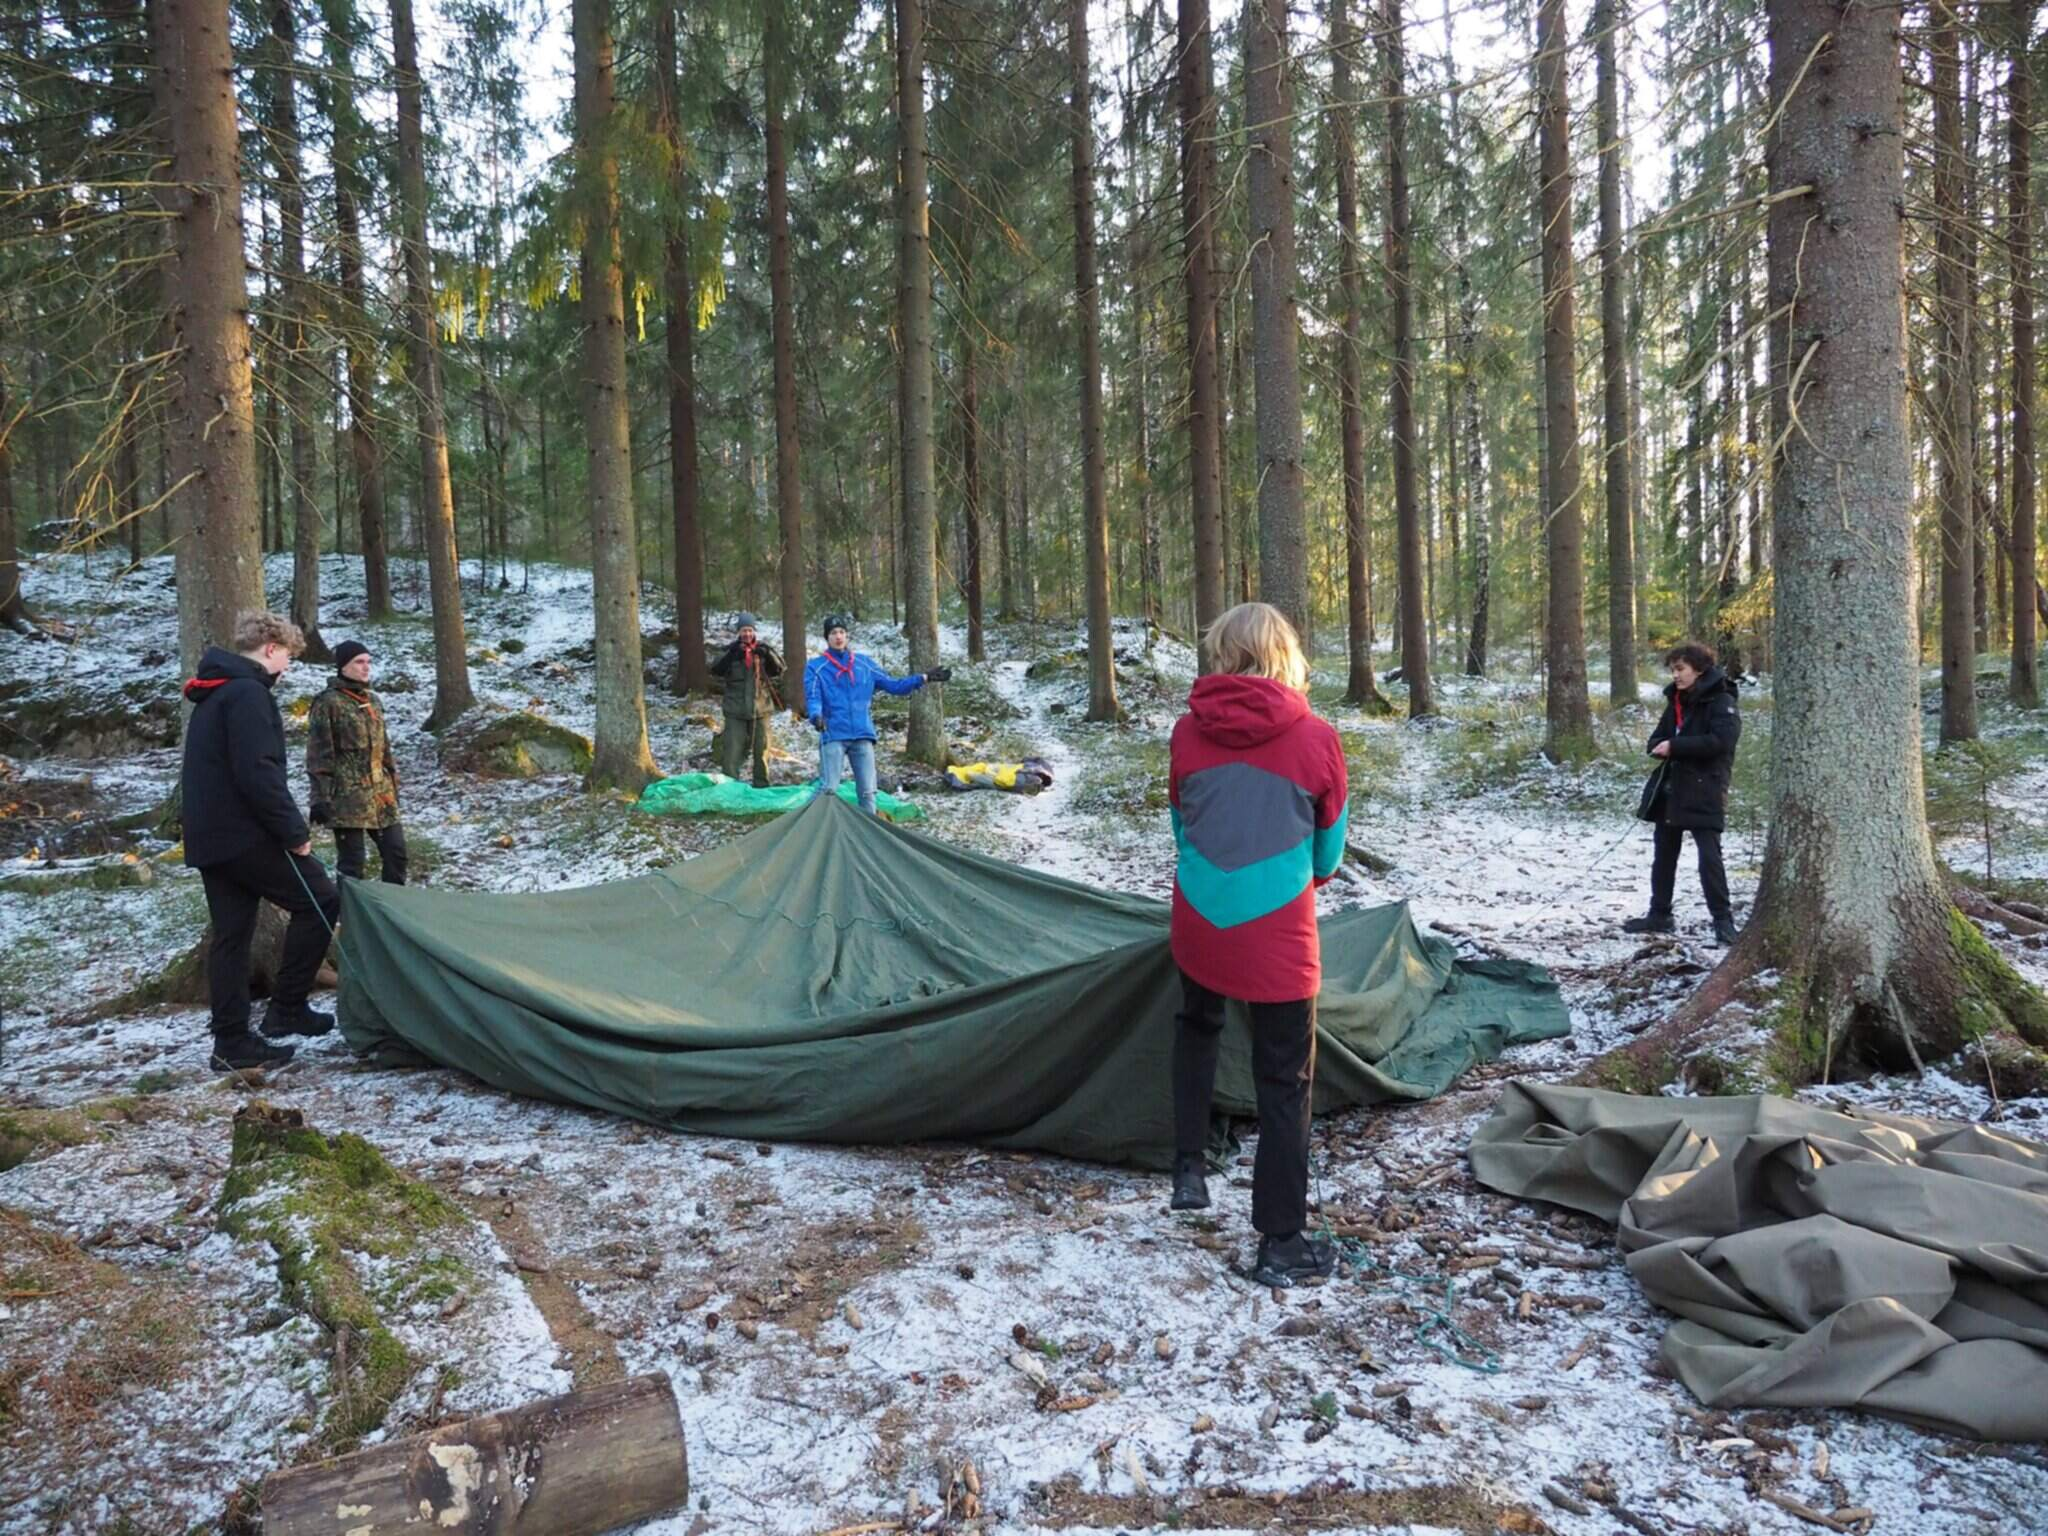
\includegraphics[width=1.0\linewidth]{assets/telttaretki4}

\begin{multicols}{2}

\noindent Huhtikuun yhdestoista päivä Kurkisuon rusakoiden seikkailijat ja tarpojat
lähtivät viileään mutta aurinkoiseen Sipoonkorpeen Bisajärven rannalle
telttailemaan ja suorittamaan kolmannen luokan riihitystä. Rusakot jakautuivat
Mikaelinkirkolla bussiosastoon sekä vanhaan tuttuun logistiikkaosastoon.
Leiriin ensimmäisenä saapui logistiikkaosasto puolijoukkueteltan, kamiinan ja
muiden varusteiden kanssa, vaikkei täysin selkeää parkkipaikkaa löytynytkään.
Hieman jäljessä saapui bussiosasto, joka väärään suuntaan mentyään ei ollut
huomannut parkkeerattua autoa.

Leiriin päästyään rusakot ryhtyivät pystyttämään puolijoukkuetelttaa,
hakkaamaan halkoja ja kaksi rusakoista pystytti oman pienemmän telttansa, koska
halusivat kokeilla sitä. Kun halot oli hakattu ja teltat kamiinaa myöten
pystytetty, menivät rusakot Bisajärven keittokatokselle syömään itse tuomiaan
iltapaloja. Kun rusakot saivat syötyä jaettiin yön kipinävuorot, minkä jälkeen
mentiin nukkumaan

\vspace*{-0.16cm}

\columnbreak

\begin{center}
	\noindent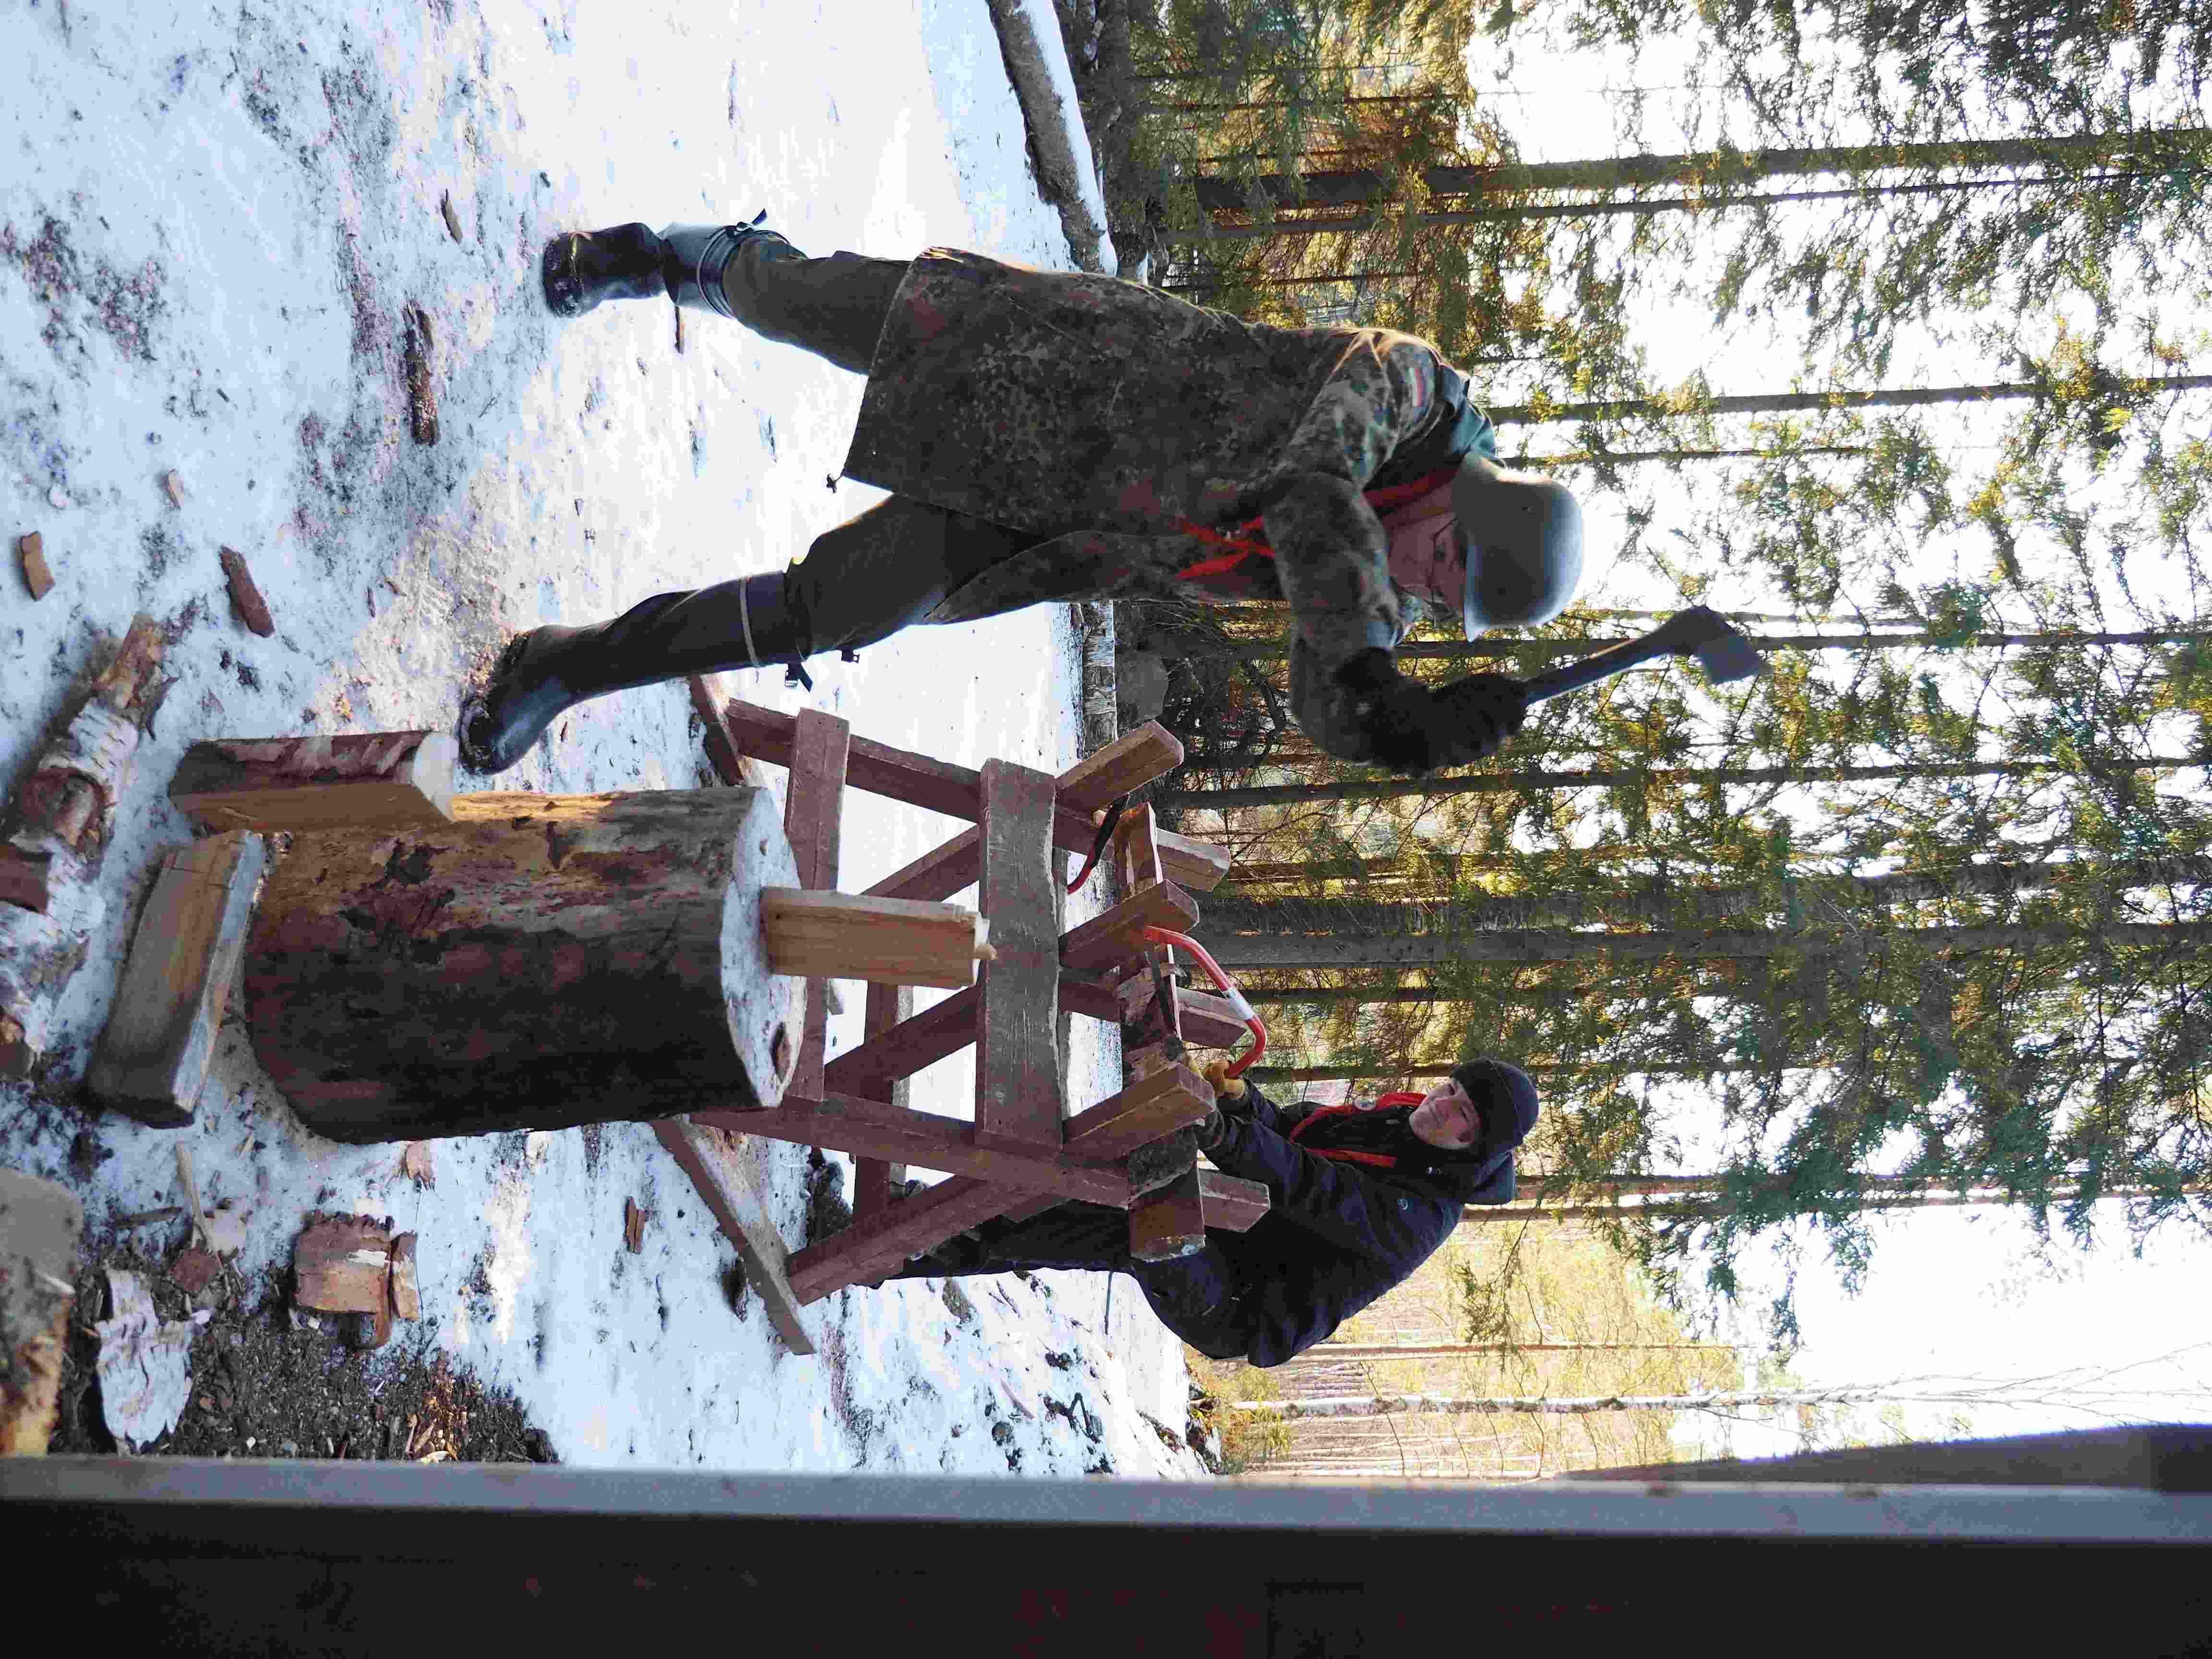
\includegraphics[height=0.9\linewidth,angle=90]{assets/telttaretki5}
\end{center}

Aamulla rusakot heräsivät lämpimälle aamupuurolle voisilmän, hillon tai
kuivattujen marjojen kera. Yön aikana oli satanut räntää, mistä huolimatta
molemmissa teltoissa oli nukuttu hyvin. Kun aamupala ja aamutoimet oli saatu
suoritettua, jaettiin vartiolaiset vartioihin ja niin saatiin riihitys
käyntiin.

Riihitys on vartioikäisten partio-ohjelmaan kuulunut suorite, joka toteutetaan
suunnistuksen muodossa. Tällä kertaa tehtävät alkoivat jo lähdöstä, jossa
vartiolaisten tehtävänä oli arvioida Bisajärven pisin halkaisija, rantaviivan
pituus sekä viereisen kukkulan korkeus järven pinnasta. Sieltä riihittäjät
suunnistivat ensimmäiselle rastille, jolla puhuttiin jokaisenoikeuksista,
eritoten tulenteosta ja siihen liittyvästä vastuusta. Toinen rasti oli
omistettu pillimerkeille, joita vartioiden tuli osata neljä kappaletta. Näihin
lukeutui esimerkiksi merkit jotka tarkoittavat “tulkaa tänne” ja “vaara.”
Kolmas rasti oli ensiapurasti, jossa riihittäjien tuli auttaa haavoittunutta
henkilöä. Neljäs rasti oli puhelinkentän ulottumattomissa oleva solmurasti.
Rastilla riihittäjien tuli tehdä merimies-, paalu- ja lippusolmu, sekä
siansorkka, ja tietää solmujen käyttötarkoitukset. Viimeisellä rastilla käytiin
läpi partioihanteita. Maalissa tehtävänä oli valmistaa vartioille lounaaksi
keittoa, josta tuli oikein hyvää ja se maistui kaikille.

\smallskip
\begin{center}
	\noindent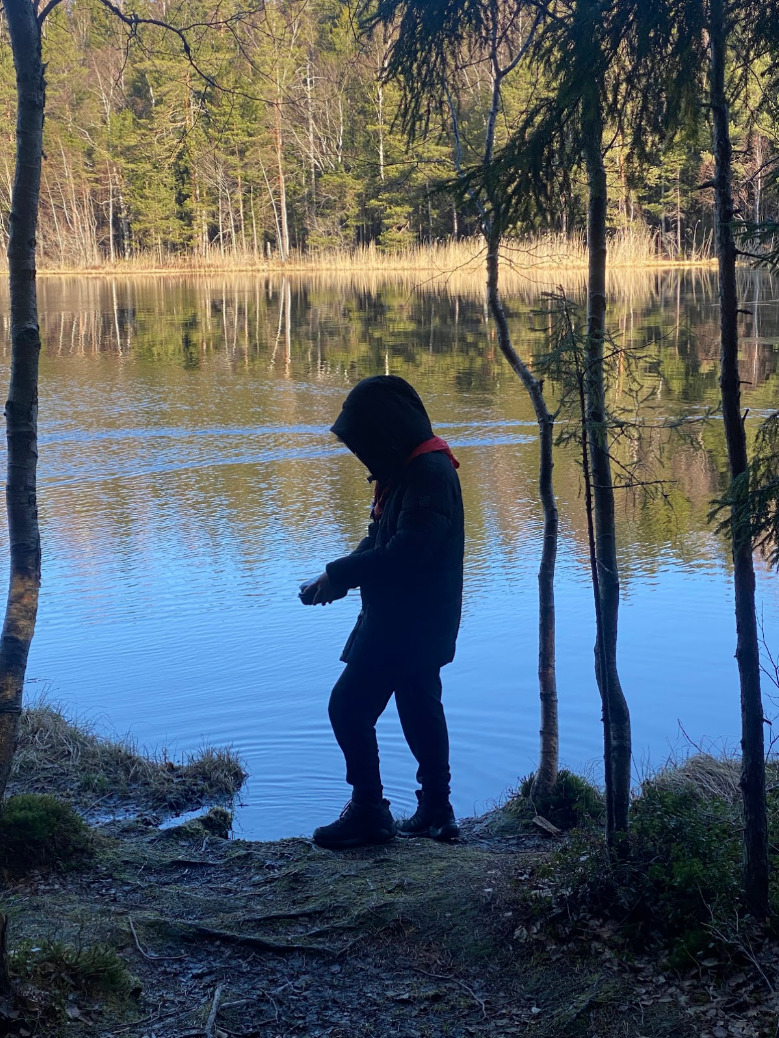
\includegraphics[width=0.9\linewidth]{assets/telttaretki1}
\end{center}

Lounaan jälkeen vartiot viimeistelivät riihityksen harjoittelemalla tulentekoa
sekä teltan kamiinalla, että risukeittimellä. Lopun iltapäivää rusakot
viettivät mitenkä halusivat, osa hakkasi halkoja ja osa vuoli makkaratikkuja,
joista muutamasta tuli hieman tarpeellista suurempia. 

\smallskip
\noindent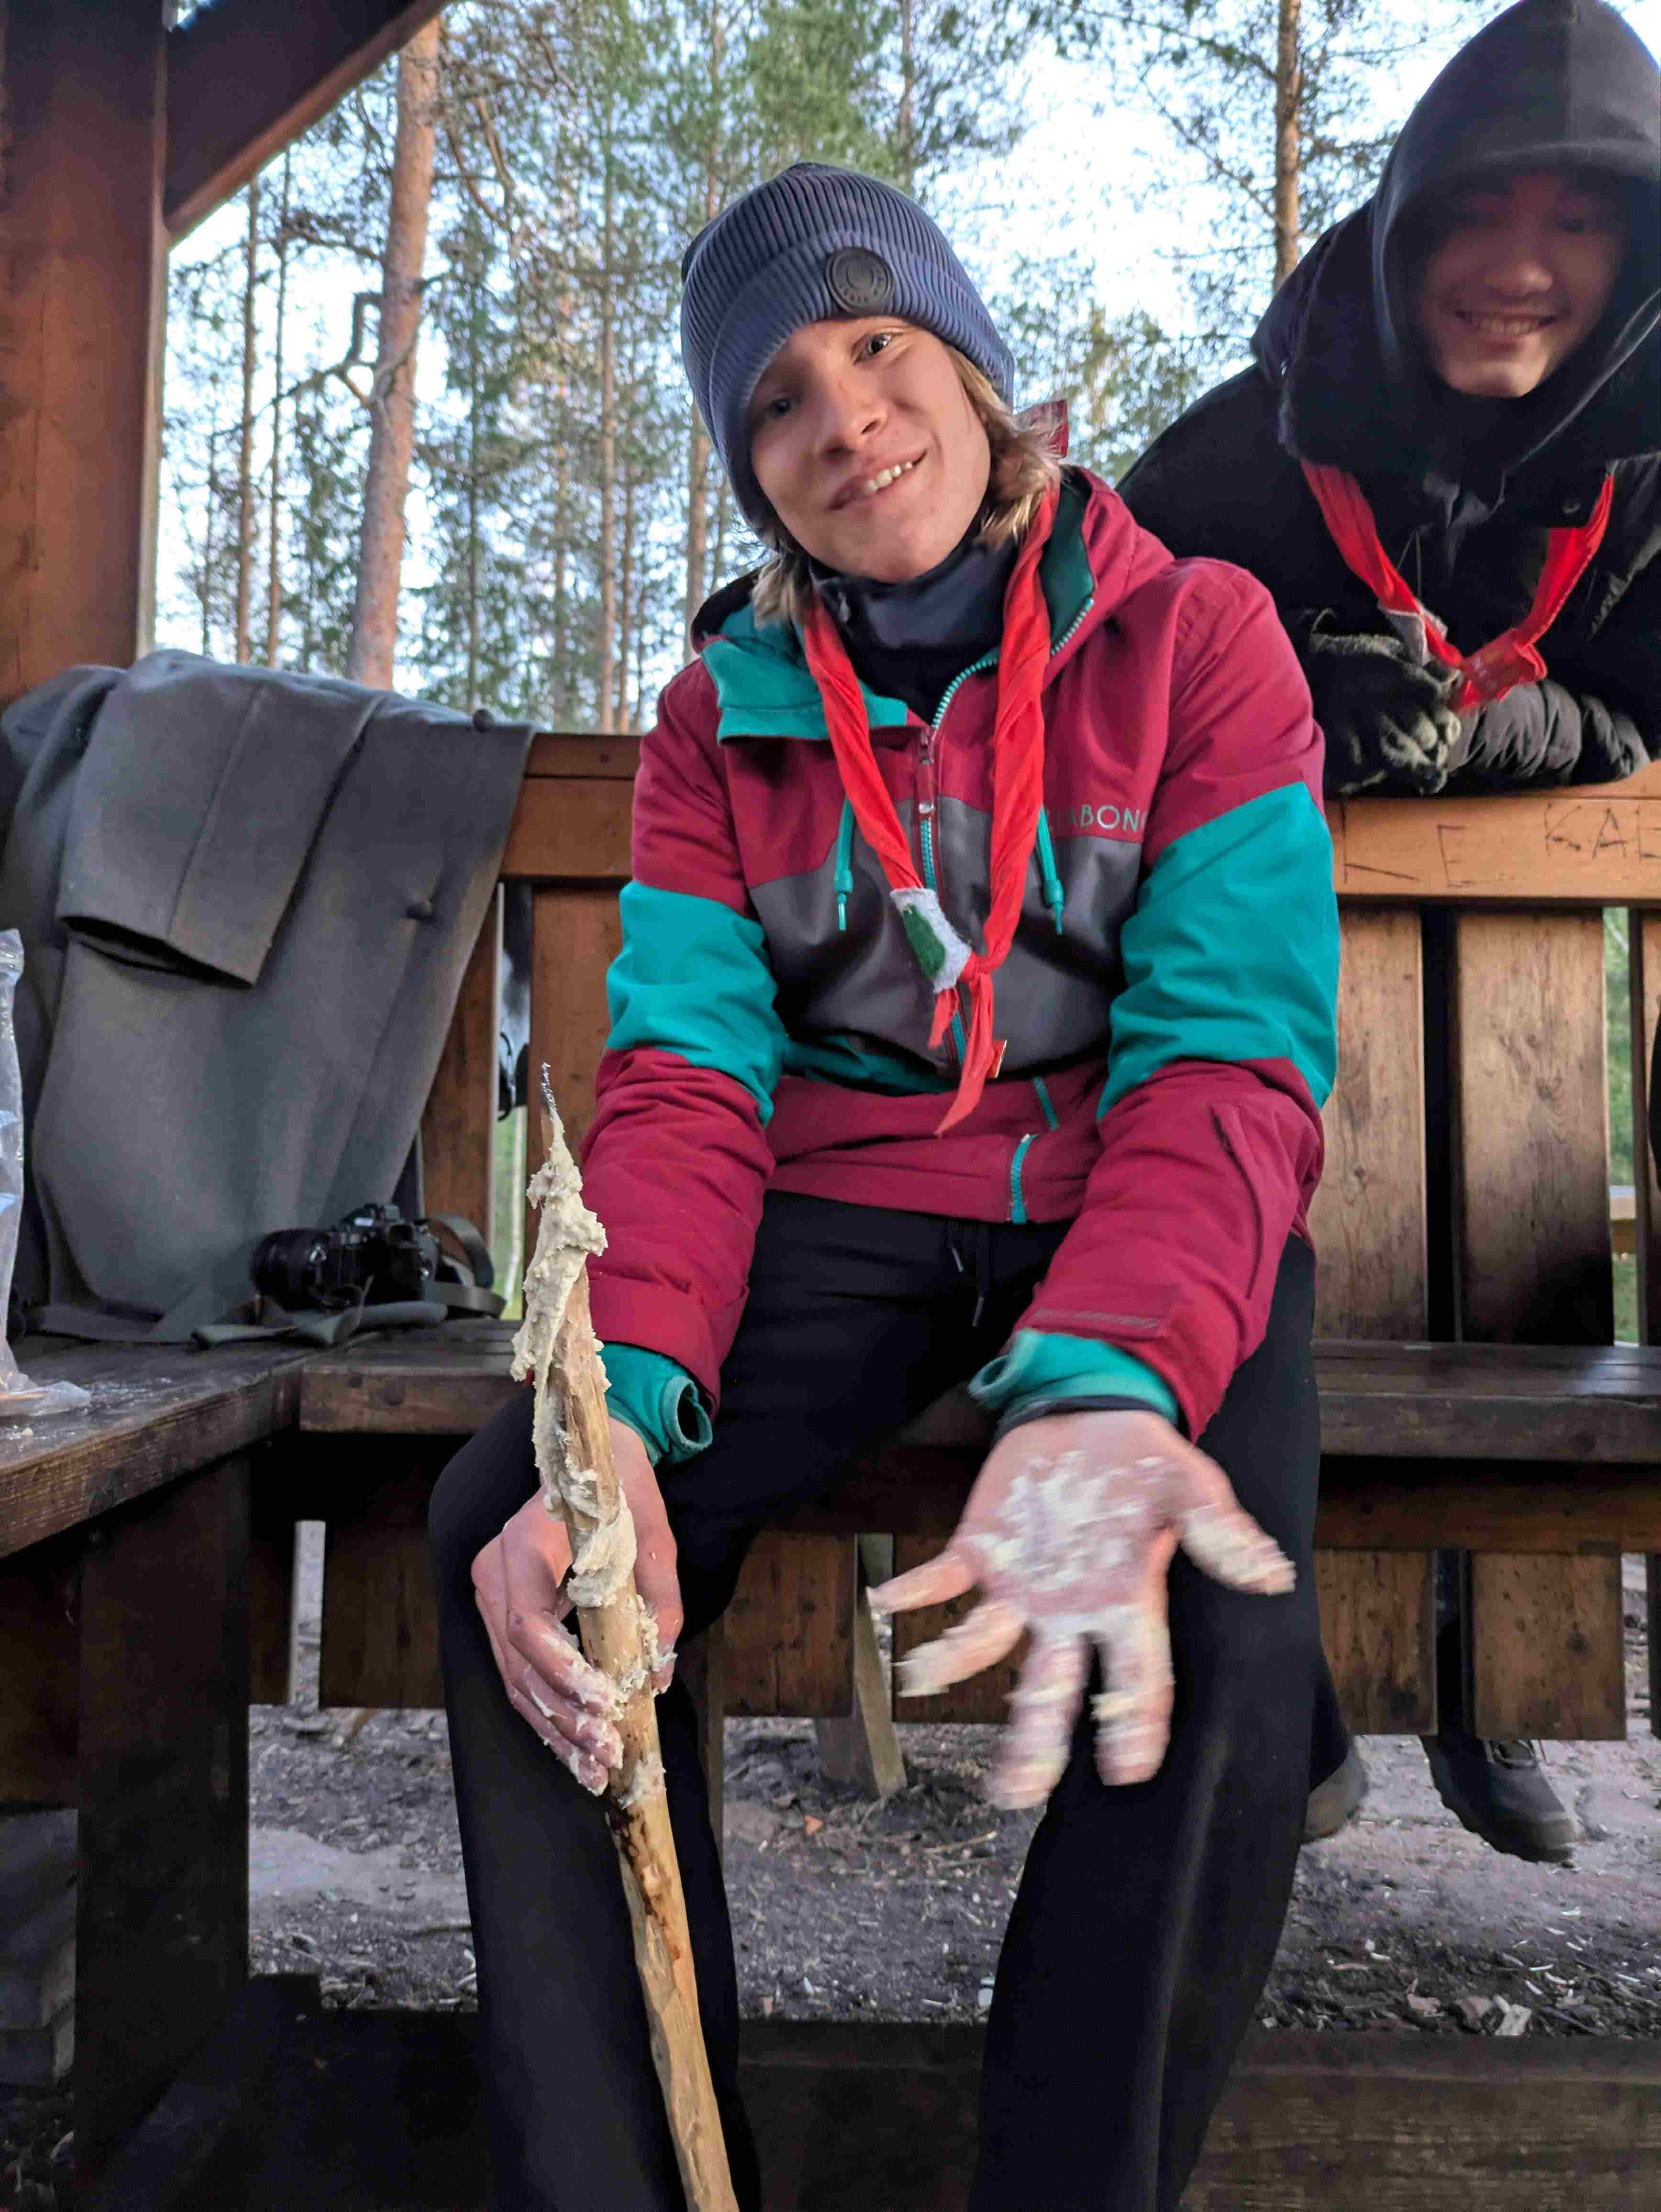
\includegraphics[width=1.0\linewidth]{assets/telttaretki3}

Makkaratikut vuoltuaan rusakot kokoontuivat jälleen keittokatokselle, jossa he
paistoivat makkaraa iltapalaksi. Makkaroiden jälkeen rusakot pääsivät myös
paistamaan tikkupullaa. Pullaa paistaessa taikina kierretään tikun ympäri, ja
paistetaan tulen yllä. Eräällä rusakolla paisto ei sujunut yhtä hyvin kun
taikina tarttui hänen käsiinsä. Iltapalan jälkeen osa rusakoista jäi vielä
keittokatokselle ihailemaan auringonlaskua, kunnes mentiin nukkumaan,

Sunnuntain vastaisena yönä kipinät sujuivat taas vaikeuksitta, mutta yöllä
leirin ohi kulki koira, joka haukkuessaan hämmästytti kipinässä olleita
rusakkoja. Sunnuntaina leirin purku aloitettiin herätyksen ja aamupalan
jälkeen. Pakatessa opeteltiin myös puolijoukkueteltan pakkaamista, joka
osoittautui osalle rusakoista oletettua vaikeammaksi. Loppujenlopuksi kaikki
saatiin pakattua, ja rusakot jakautuivat jälleen bussiosastoon sekä
logistiikkaosastoon. Logistiikkaosaston koko vahvuus eli seitsemän rusakkoa
survoutui alkumatkaksi yhteen autoon kaluston kanssa, jolloin muun muassa
rinkat kulkivat ensimmäiset kilometrit sylissä, kunnes osa rusakoista jätti
logistiikkaosaston ja hyppäsi bussiin kotia kohti.

\smallskip
\noindent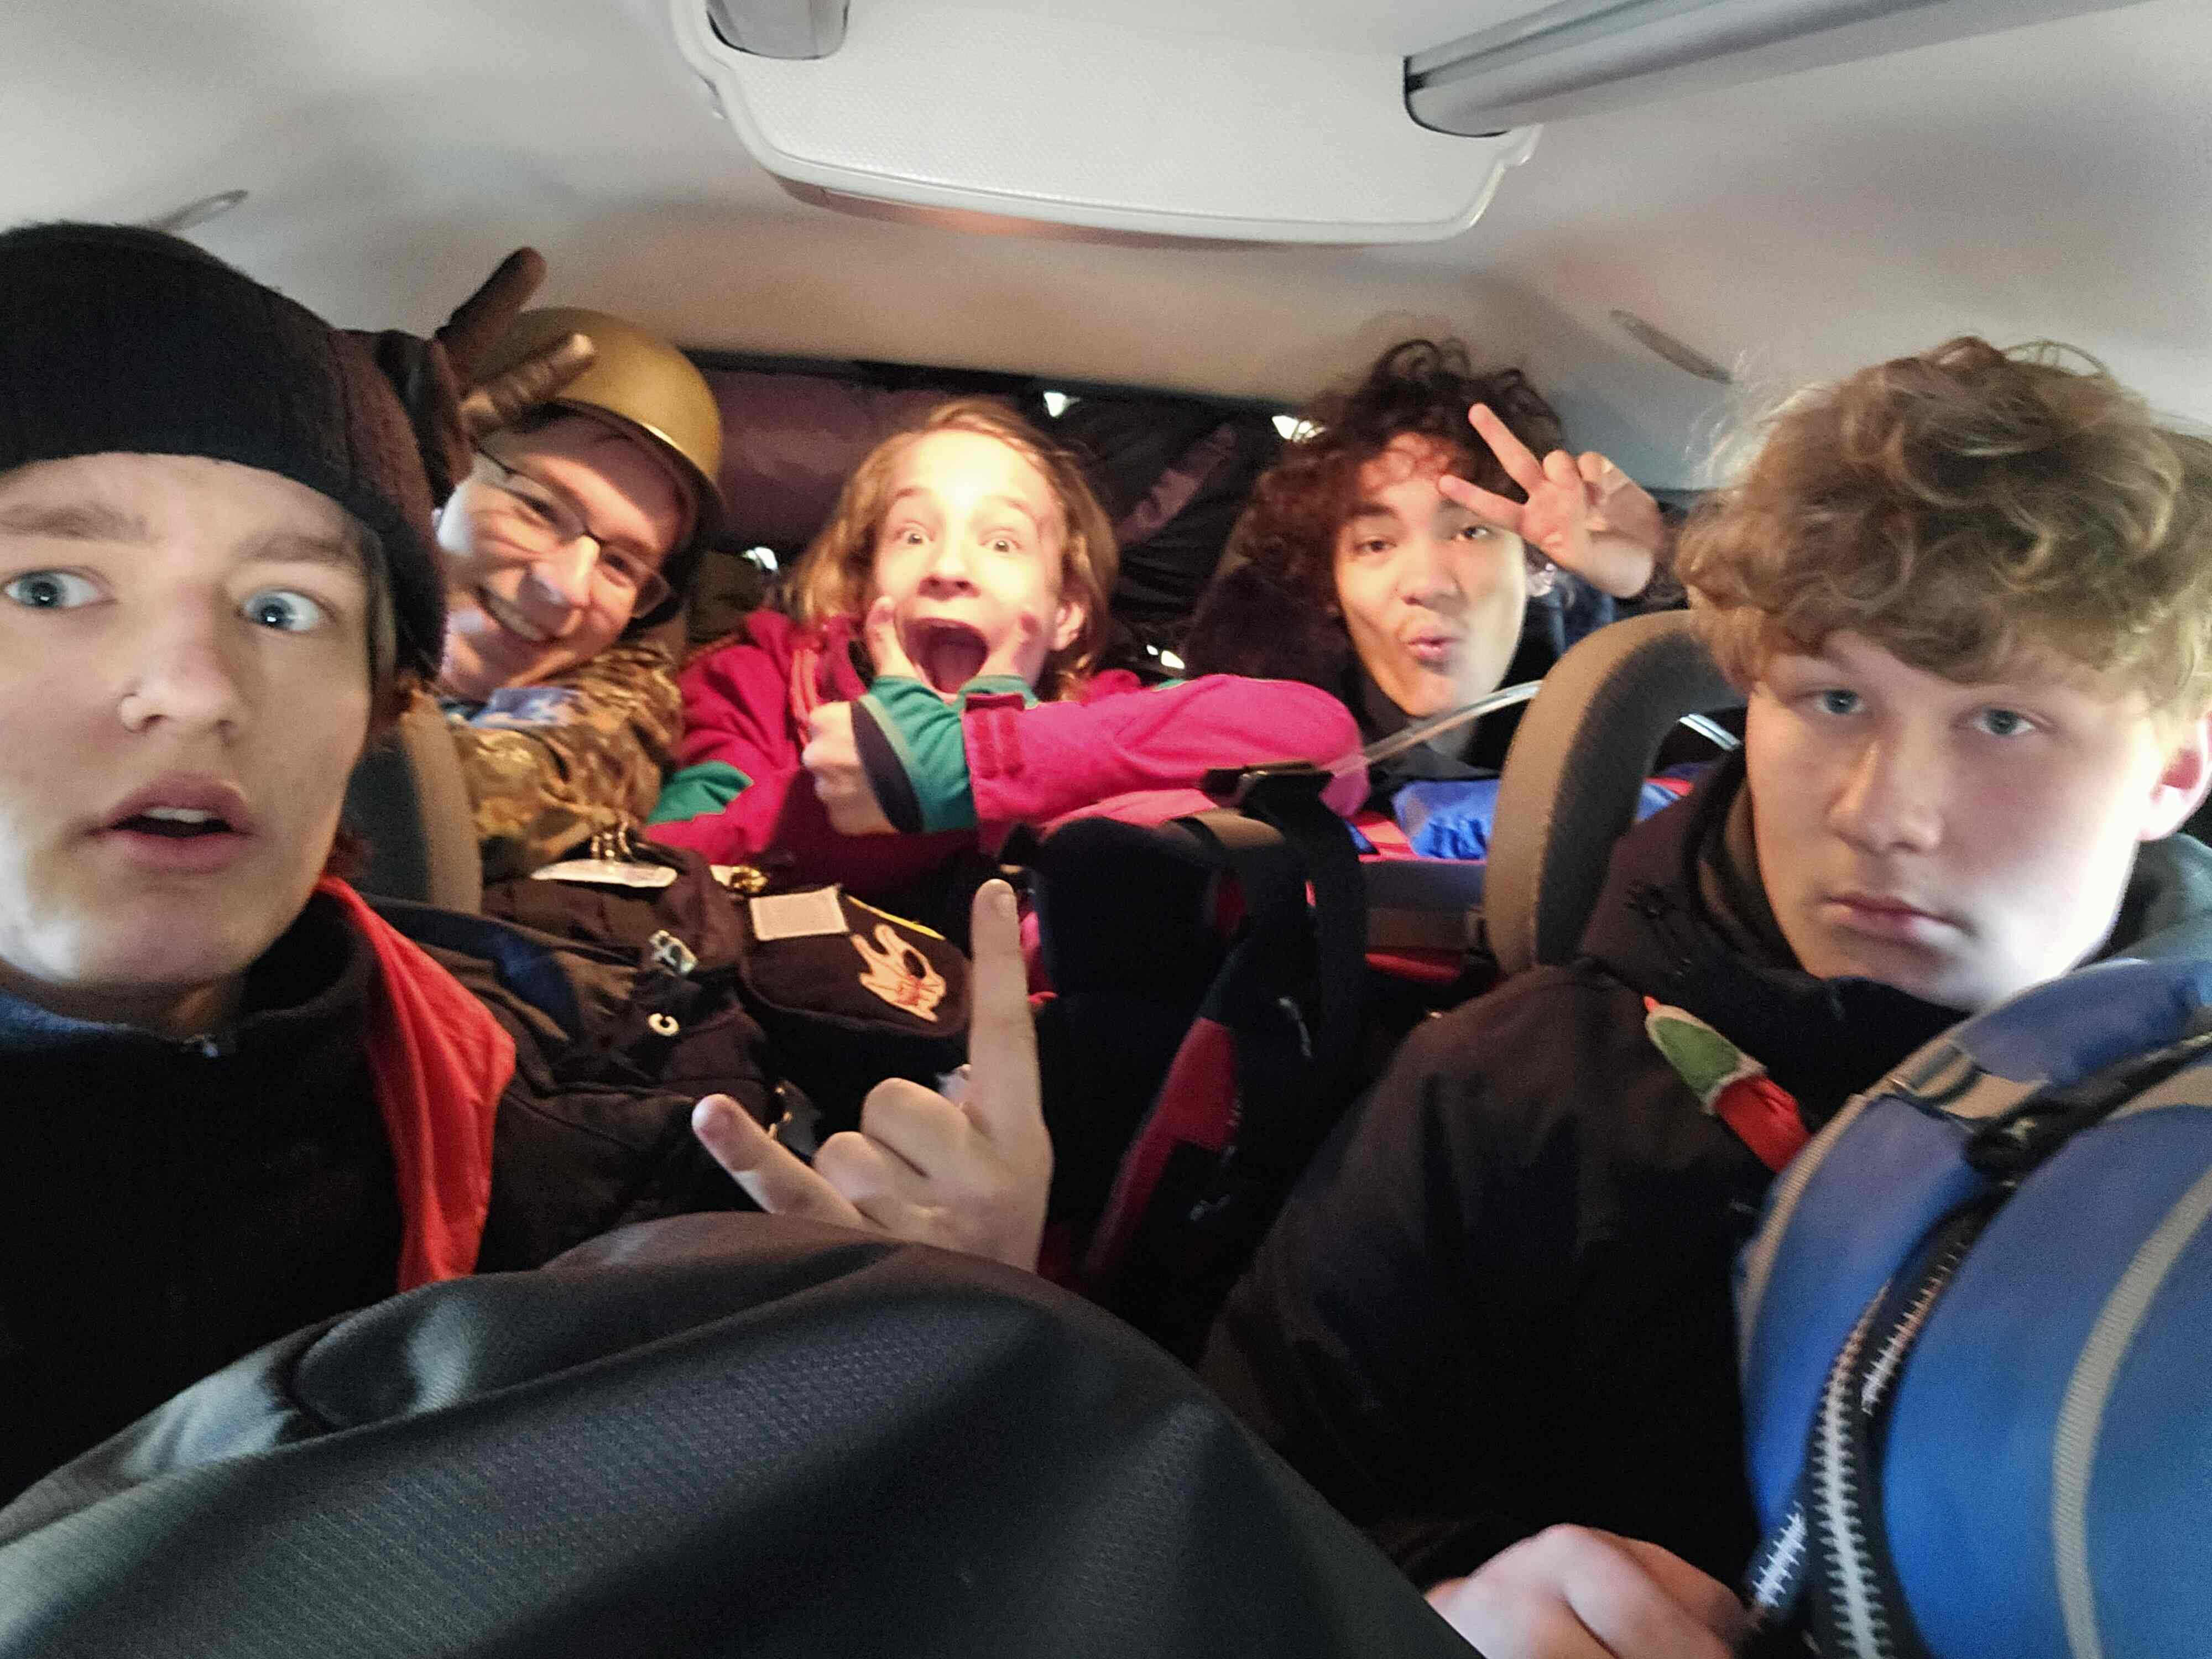
\includegraphics[width=1.0\linewidth]{assets/telttaretki2}

\end{multicols}

\noindent\null\hfill Texti: Päärynä-Hyttyset\\
\noindent\null\hfill Kuvat: PäHy, Leo \& Tanguy\\


\section{Kevätjuhlassa ansioituneet}

\begin{figure}[!b]
\centering\includegraphics[width=\textwidth]{example-image-a}
\caption{Blaa blaa blaa.}
\end{figure}

\begin{multicols}{2}
\noindent Lippukunnan kevätjuhla järjestettiin perinteikkäästi leikkipuisto Kipinäpuistossa jo tutussa ''amfiteatterissa''. Juhlassa jaettiin parven ja vartioiden keväällä suorittamia merkkejä.

Ilmastosankari- ja liikunta"-jäljet: \textit{Kurjet}"-parvi (x).

Länsi"-ilmansuunta: \textit{Pomppupallot}"-vartio (x).

Yhteiskunta"-tarppo: \textit{Päärynähyttyset}"-vartio (x).

Vihreä nahkalilja: x

Punainen nahkalilja: x

Harmaa nahkalilja: x

Aktiivisimman kolkan kiertopalkinto: x

Kiitos"-pinssi: x
\end{multicols}

\medskip

\noindent\null\hfill Kuva: x\\ 
\noindent\null\hfill Teksti: Janne


% \section{Johtajien kansallispuistokierros Ruotsissa}


% \section{Muistoja vuodelta 2024: Uikun uinti -vaellus 26.–30.6.}

%Pending the interviews so commented for now. Move maybe to 2/2025.
%\section{Partiomenetelmä? KESKEN}

\textit{Varsin usein kuulee kysyttävän, mitä partio on. Partiomenetelmä tekee partiosta partiota. Tassun 1/2008 partioihannejutun ja Suomen Partiolaisten jäsenkokouksen 16.--17.11.2024 hyväksymän partiomenetelmäuudistuksen innoittamina Tassun toimitus kysyi rusakoilta esimerkkejä, miten partiomenetelmän eri osa"-alueet ovat näkyneet heidän toiminnassaan.}

\begin{multicols}{2}
\noindent\textbf{Lupaus, tunnus ja ihanteet}. {\small Partiolaisen lupaus, tunnus ja ihanteet kuvaavat partion arvoja. Partiolainen pyrkii toimimaan näiden arvojen mukaisesti.\par}

\medskip\noindent\textbf{Symboliikka}. {\small Partion symboliikka muodostuu yhteisesti merkityksellisiksi koettujen toimintatapojen ja tunnusten kokonaisuudesta. Symboliikka tukee oman, ryhmän ja yhteisön identiteetin kehittymistä.\par}

\medskip\noindent\textbf{Oma partiopolku}. {\small Innostava ja sopivan haastava toiminta auttaa kasvamaan ja kehittymään omalla partiopolulla. Partiossa opitaan yksin ja yhdessä taitoja elämää varten.\par}

\medskip\noindent\textbf{Ryhmässä toimiminen}. {\small Partiossa toimitaan vertaisryhmissä, joissa tehdään päätöksiä ja kannetaan vastuuta yhdessä. Oma ryhmä on turvallinen ympäristö harjoitella johtajuutta ja vuorovaikutusta.\par}

\medskip\noindent\textbf{Tekemällä oppiminen}. {\small Partiossa opitaan yhdessä kokemalla ja tekemällä. Etukäteen suunnittelu ja jälkikäteen reflektointi tukevat oppimista.\par}

\medskip\noindent\textbf{Aikuinen tuki}. {\small Partio on nuorten liike, mitä aikuiset tukevat. Aikuinen tukee lapsen ja nuoren yksilöllistä kasvua, osallistumista sekä vaikuttamismahdollisuuksia kuunnellen ja auttaen.\par}

\medskip\noindent\textbf{Hyvän tekeminen}. {\small Partiossa opitaan kantamaan vastuuta itsestä ja muista. Partiolainen rakentaa parempaa maailmaa, on aktiivinen kansalainen ja toimii yhdessä muiden kanssa yhteisöjensä hyväksi.\par}

\medskip\noindent\textbf{Toiminta luonnossa}. {\small Luonto on partiossa keskeisin kasvamisympäristö. Luonnossa toimiminen rakentaa henkilökohtaista luontosuhdetta.\par}

\medskip\noindent\textbf{Elämyksellisyys}. {\small Partiossa koetaan pieniä ja suuria elämyksiä sekä seikkailuja erilaisissa ympäristöissä. Partio tarjoaa mahdollisuuden pitää hauskaa yhdessä.\par}
\end{multicols}

\medskip

\noindent\null\hfill Kuvat: ???\\
\noindent\null\hfill Lähteet: SP:n peruskirja


% 
\section{Salaperäinen viesti}

\setlength\tabcolsep{-2pt}
	\begin{table*}[h]
	\small\centering
\makebox[0.94\textwidth][c]{%
	\begin{tabular}{|ccccccccccccccccc|ccccccccccccccccc|}
	\hline
	\multicolumn{16}{|c|}{\makecell{\morse{E} \\ E}} & \multicolumn{16}{c|}{\makecell{\morse{T} \\ T}} \\ \hline
	\multicolumn{8}{|c|}{\makecell{\morse{I} \\ I}} & \multicolumn{8}{c|}{\makecell{\morse{A} \\ A}} & \multicolumn{8}{c|}{\makecell{\morse{N} \\ N}} & \multicolumn{8}{c|}{\makecell{\morse{M} \\ M}} \\ \hline
	\multicolumn{4}{|c|}{\makecell{\morse{S} \\ S}} & \multicolumn{4}{c|}{\makecell{\morse{U} \\ U}} & \multicolumn{4}{c|}{\makecell{\morse{R} \\ R}} & \multicolumn{4}{c|}{\makecell{\morse{W} \\ W}} & \multicolumn{4}{c|}{\makecell{\morse{D} \\ D}} & \multicolumn{4}{c|}{\makecell{\morse{K} \\ K}} & \multicolumn{4}{c|}{\makecell{\morse{G} \\ G}} & \multicolumn{4}{c|}{\makecell{\morse{O} \\ O}} \\ \hline
	\multicolumn{2}{|c|}{\makecell{\morse{H} \\ H}} & \multicolumn{2}{c|}{\makecell{\morse{V} \\ V}} &
	\multicolumn{2}{c|}{\makecell{\morse{F} \\ F}} & \multicolumn{2}{c|}{\makecell{\morseprosign{IM} \\ Ü}} &
	\multicolumn{2}{c|}{\makecell{\morse{L} \\ L}} & \multicolumn{2}{c|}{\makecell{\morse{Ä} \\ Ä}} &
	\multicolumn{2}{c|}{\makecell{\morse{P} \\ P}} & \multicolumn{2}{c|}{\makecell{\morse{J} \\ J}} &
	\multicolumn{2}{c|}{\makecell{\morse{B} \\ B}} & \multicolumn{2}{c|}{\makecell{\morse{X} \\ X}} &
	\multicolumn{2}{c|}{\makecell{\morse{C} \\ C}} & \multicolumn{2}{c|}{\makecell{\morse{Y} \\ Y}} &
	\multicolumn{2}{c|}{\makecell{\morse{Z} \\ Z}} & \multicolumn{2}{c|}{\makecell{\morse{Q} \\ Q}} &
	\multicolumn{2}{c|}{\makecell{\morse{Ö} \\ Ö}} & \multicolumn{2}{c|}{\makecell{\morseprosign{MM} \\ -{}-{}-}} \\
	\hline
	% \multicolumn{1}{|c|}{\morse{}} & \multicolumn{1}{c|}{\morse{}} & \multicolumn{1}{c|}{\morse{}} & \multicolumn{1}{c|}{\morse{}} & \multicolumn{1}{c|}{\morse{}} & \multicolumn{1}{c|}{\morse{}} & \multicolumn{1}{c|}{\morse{}} & \multicolumn{1}{c|}{\morse{}} & \multicolumn{1}{c|}{\morse{}} & \multicolumn{1}{c|}{\morse{}} & \multicolumn{1}{c|}{\morse{}} & \multicolumn{1}{c|}{\morse{}} & \multicolumn{1}{c|}{\morse{}} & \multicolumn{1}{c|}{\morse{}} & \multicolumn{1}{c|}{\morse{}} & \multicolumn{1}{c|}{\morse{}} & \multicolumn{1}{c|}{\morse{}} & \multicolumn{1}{c|}{\morse{}} & \multicolumn{1}{c|}{\morse{}} & \multicolumn{1}{c|}{\morse{}} & \multicolumn{1}{c|}{\morse{}} & \multicolumn{1}{c|}{\morse{}} & \multicolumn{1}{c|}{\morse{}} & \multicolumn{1}{c|}{\morse{}} & \multicolumn{1}{c|}{\morse{}} & \multicolumn{1}{c|}{\morse{}} & \multicolumn{1}{c|}{\morse{}} & \multicolumn{1}{c|}{\morse{}} & \multicolumn{1}{c|}{\morse{}} & \multicolumn{1}{c|}{\morse{}} & \multicolumn{1}{c|}{\morse{}} & \multicolumn{1}{c|}{\morse{}} \\ \hline
	\end{tabular}%
}
\caption{Muistitaulukko Morsen kirjaimille, \cite{scoutwikimorse}}
% \caption{Muistitaulukko Morsen kirjaimille ja numeroille}
\end{table*}

\noindent\daaah{4cm}\morseprosign{?}\\
\noindent\morse{ABCDEFGHIJKLMNO}\\
\noindent\morse{PQRSTUVWXYZÅÄÖ}\\
\noindent\morse{0123456789}\\
\noindent\morse{?/=:,.}\\


%TIP COLUMNS
\include{chapters/kesäretkeilyvinkit.tex}

%COMPETITIONS

\section{Kuvakilpailun hedelmiä}

\textit{Koska \textit{Vene}-samoajavartio ei osallistunut, heidät nostettiin kuvakilpailun tuomaristoksi. Heidän pohdintansa jälkeen tässä ovat kilpailun tulokset.}

\vspace{0.64cm}

\begin{multicols}{2}

% \vspace*{-0.32cm}
	\subsection*{3. paikka:}
\begin{center}
	\noindent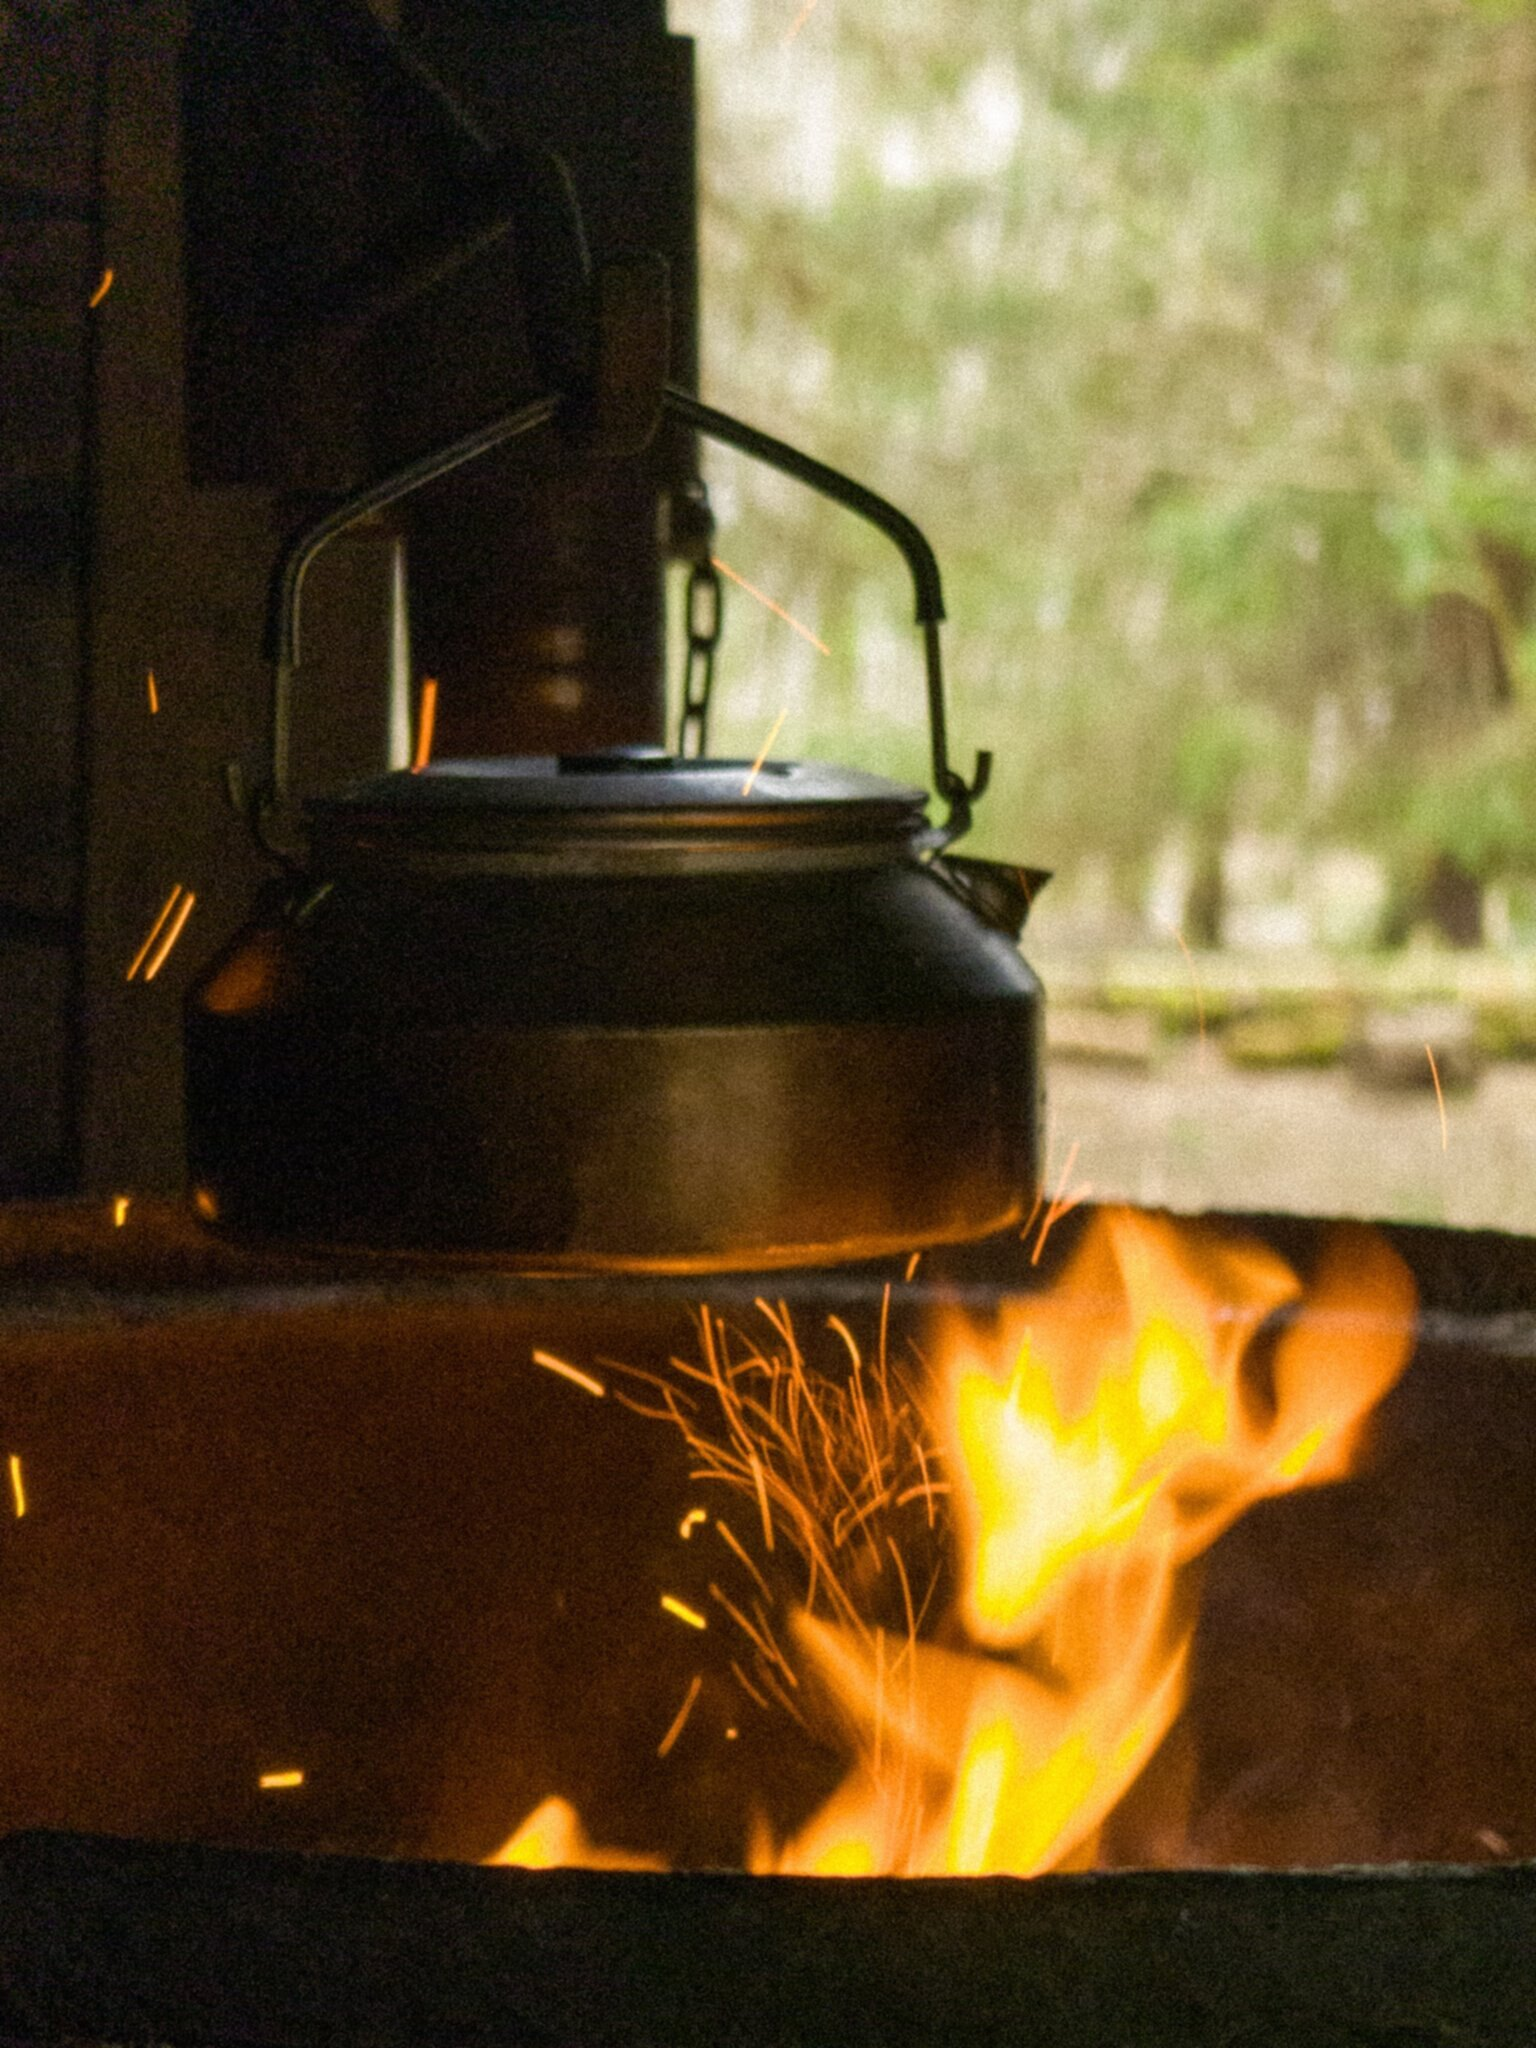
\includegraphics[height=0.9\linewidth]{assets/kuvakilpailu3}\\
	``Kahvii'' - Mikko% Niinimäki
\end{center}

\columnbreak

% \vspace*{-0.16cm}
	\subsection*{2. paikka:}
	\vspace*{0.54cm}
\begin{center}
	\noindent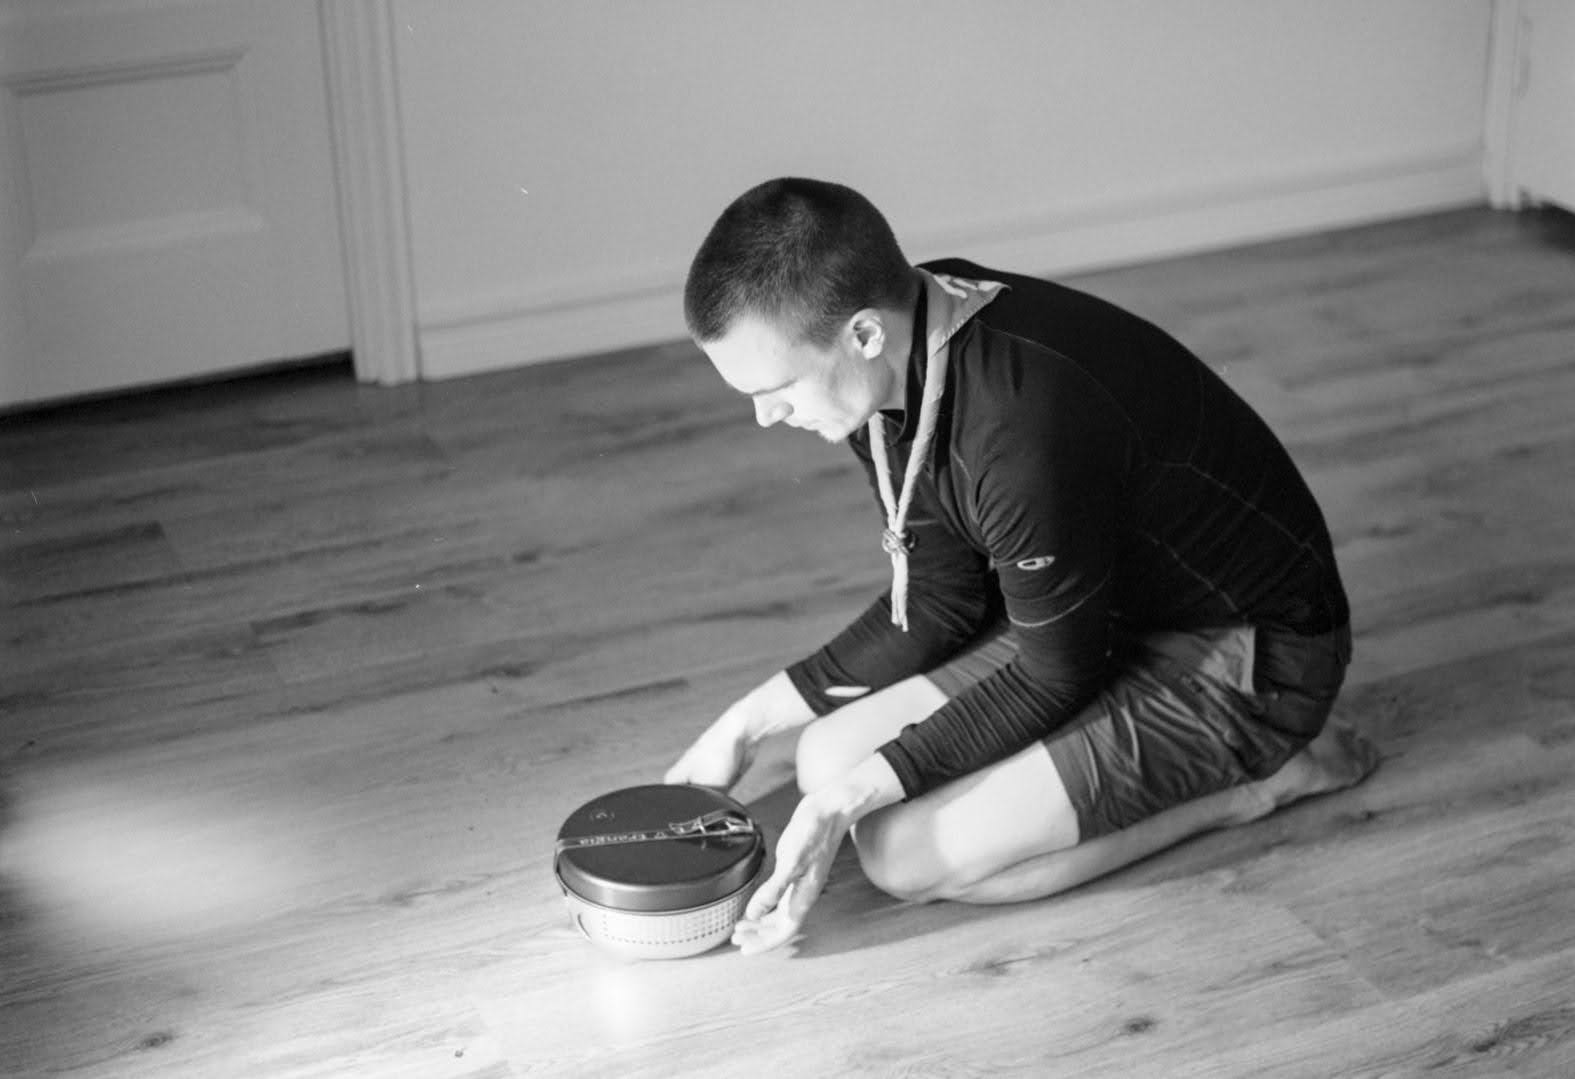
\includegraphics[width=0.99\linewidth]{assets/kuvakilpailu2}\\
	``Mies ja retkikeitin'' - Janne% Suomalainen
	\vspace*{0.54cm}
\end{center}

\end{multicols}

\begin{multicols}{2}

	\noindent Lähteet: \quad --

	\noindent Tuomariston keskiarvo: 2,5/5

	\columnbreak

	\noindent Lähteet: Poika ja pääkallo\\ \hfill - Magnus Enckell

	\noindent Tuomariston keskiarvo: 3,75/5

\end{multicols}

\begin{multicols}{2}

\noindent Kuva itsessään on oikein hieno ja se voisi sopia erinomaisesti Tassuun esim.
artikkelin kuvitukseksi. Kuva on sopivan yksinkertainen ja tunnelmallinen ja
kuvaa hyvin sitä, miltä kahvin juominen metsäretkellä tuntuu. Kuitenkin
kuvakilpailun tehtävänannon se ohittaa, sillä se ei viittaa mihinkään
taideteokseen, eikä näin ollen ole kilpailun sääntöjen mukainen.

	\columnbreak

\noindent Kuvan idea on luova ja kuvaan otettu retkikeitin myös lisää siihen
asiaankuuluvaa partiotunnelmaa. Asetelma mukailee hienosti alkuperäistä
taideteosta. Kuvan valotus on paikoittain hieman liian kirkas. Kuva on hyvin
yksinkertainen ja vaikka se ei olekaan huono asia, raati jäi kaipaamaan jotakin
elementtiä, joka olisi kiinnittänyt katsojan mielenkiinnon paremmin, minkä
vuoksi se jäi hitusen alle voittopisteiden.

\end{multicols}

\clearpage
% \vspace*{0.64cm}
\subsection*{1. paikka:}
\begin{center}
	\noindent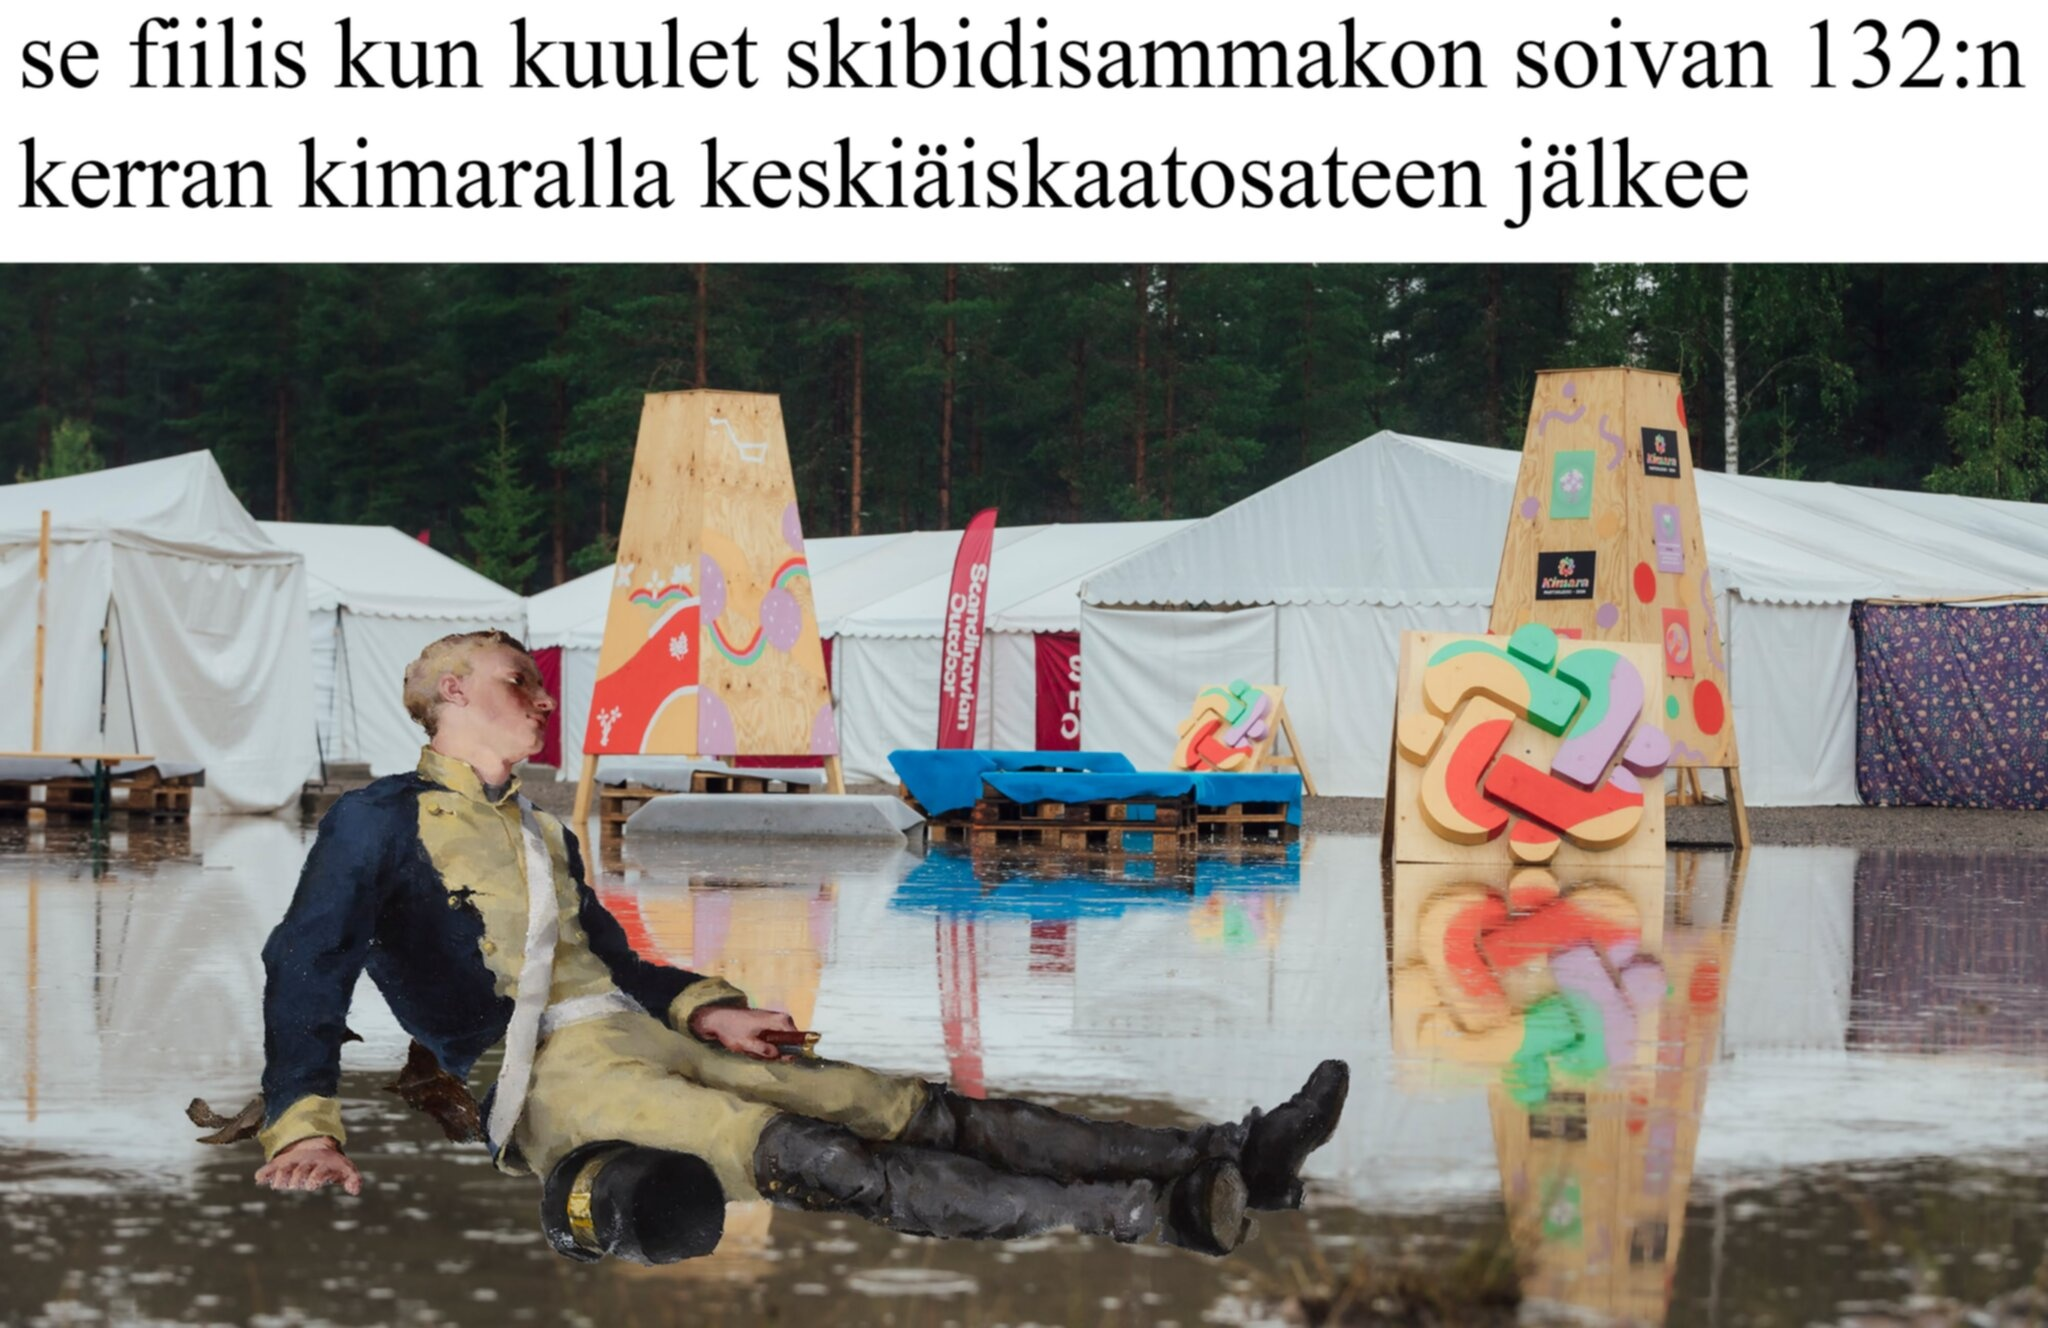
\includegraphics[width=1.0\linewidth]{assets/kuvakilpailu1}\\
	``rip bro.png'' - Alden% Forsström
\end{center}

\noindent Lähteet: \quad Haavoittunut Soturi Hangessa - Helene Schjerfbeck

\qquad\qquad Hanna Hämäläisen kuva, PäPa:n kuvapankistä

\bigskip
\noindent Tuomariston keskiarvo: 3,875/5\\
\noindent Eliaksen arvio: ``5/5 absolute cinema''

\bigskip
\noindent Kuva vetosi raatiin, sillä suurin osa pystyi samaistumaan siinä
kuvattuun tuskaan ja epätoivoon. Myös raadin iän ja kypsyyden huomioon ottaen
ei tule yllätyksenä, että meemiformaatti keräsi eniten pisteitä. Hauskuutta
kuvaan lisää se, että sen taustana on käytetty oikeaa kuvaa kuvatusta
tilanteesta. Tekijältä kuitenkin meni ohi oiva mahdollisuus käyttää numeroa
104, jolloin kuvasta olisi tullut entistä moniulotteisempi. Myös kuvatekstin
kielelliseen asuun olisi voinut panostaa enemmän. Kuva ei myöskään aukea
yleisölle, joka ei ollut Kimaralla kokemassa kuvattua tilannetta ja tästä
syystä myös tuomariston pisteiden keskiarvo laski.


\section{Neulesuunnittelukilpailu}\label{sec:neulekilpailu}

\begin{wrapfigure}{r}{0.25\textwidth}
	\noindent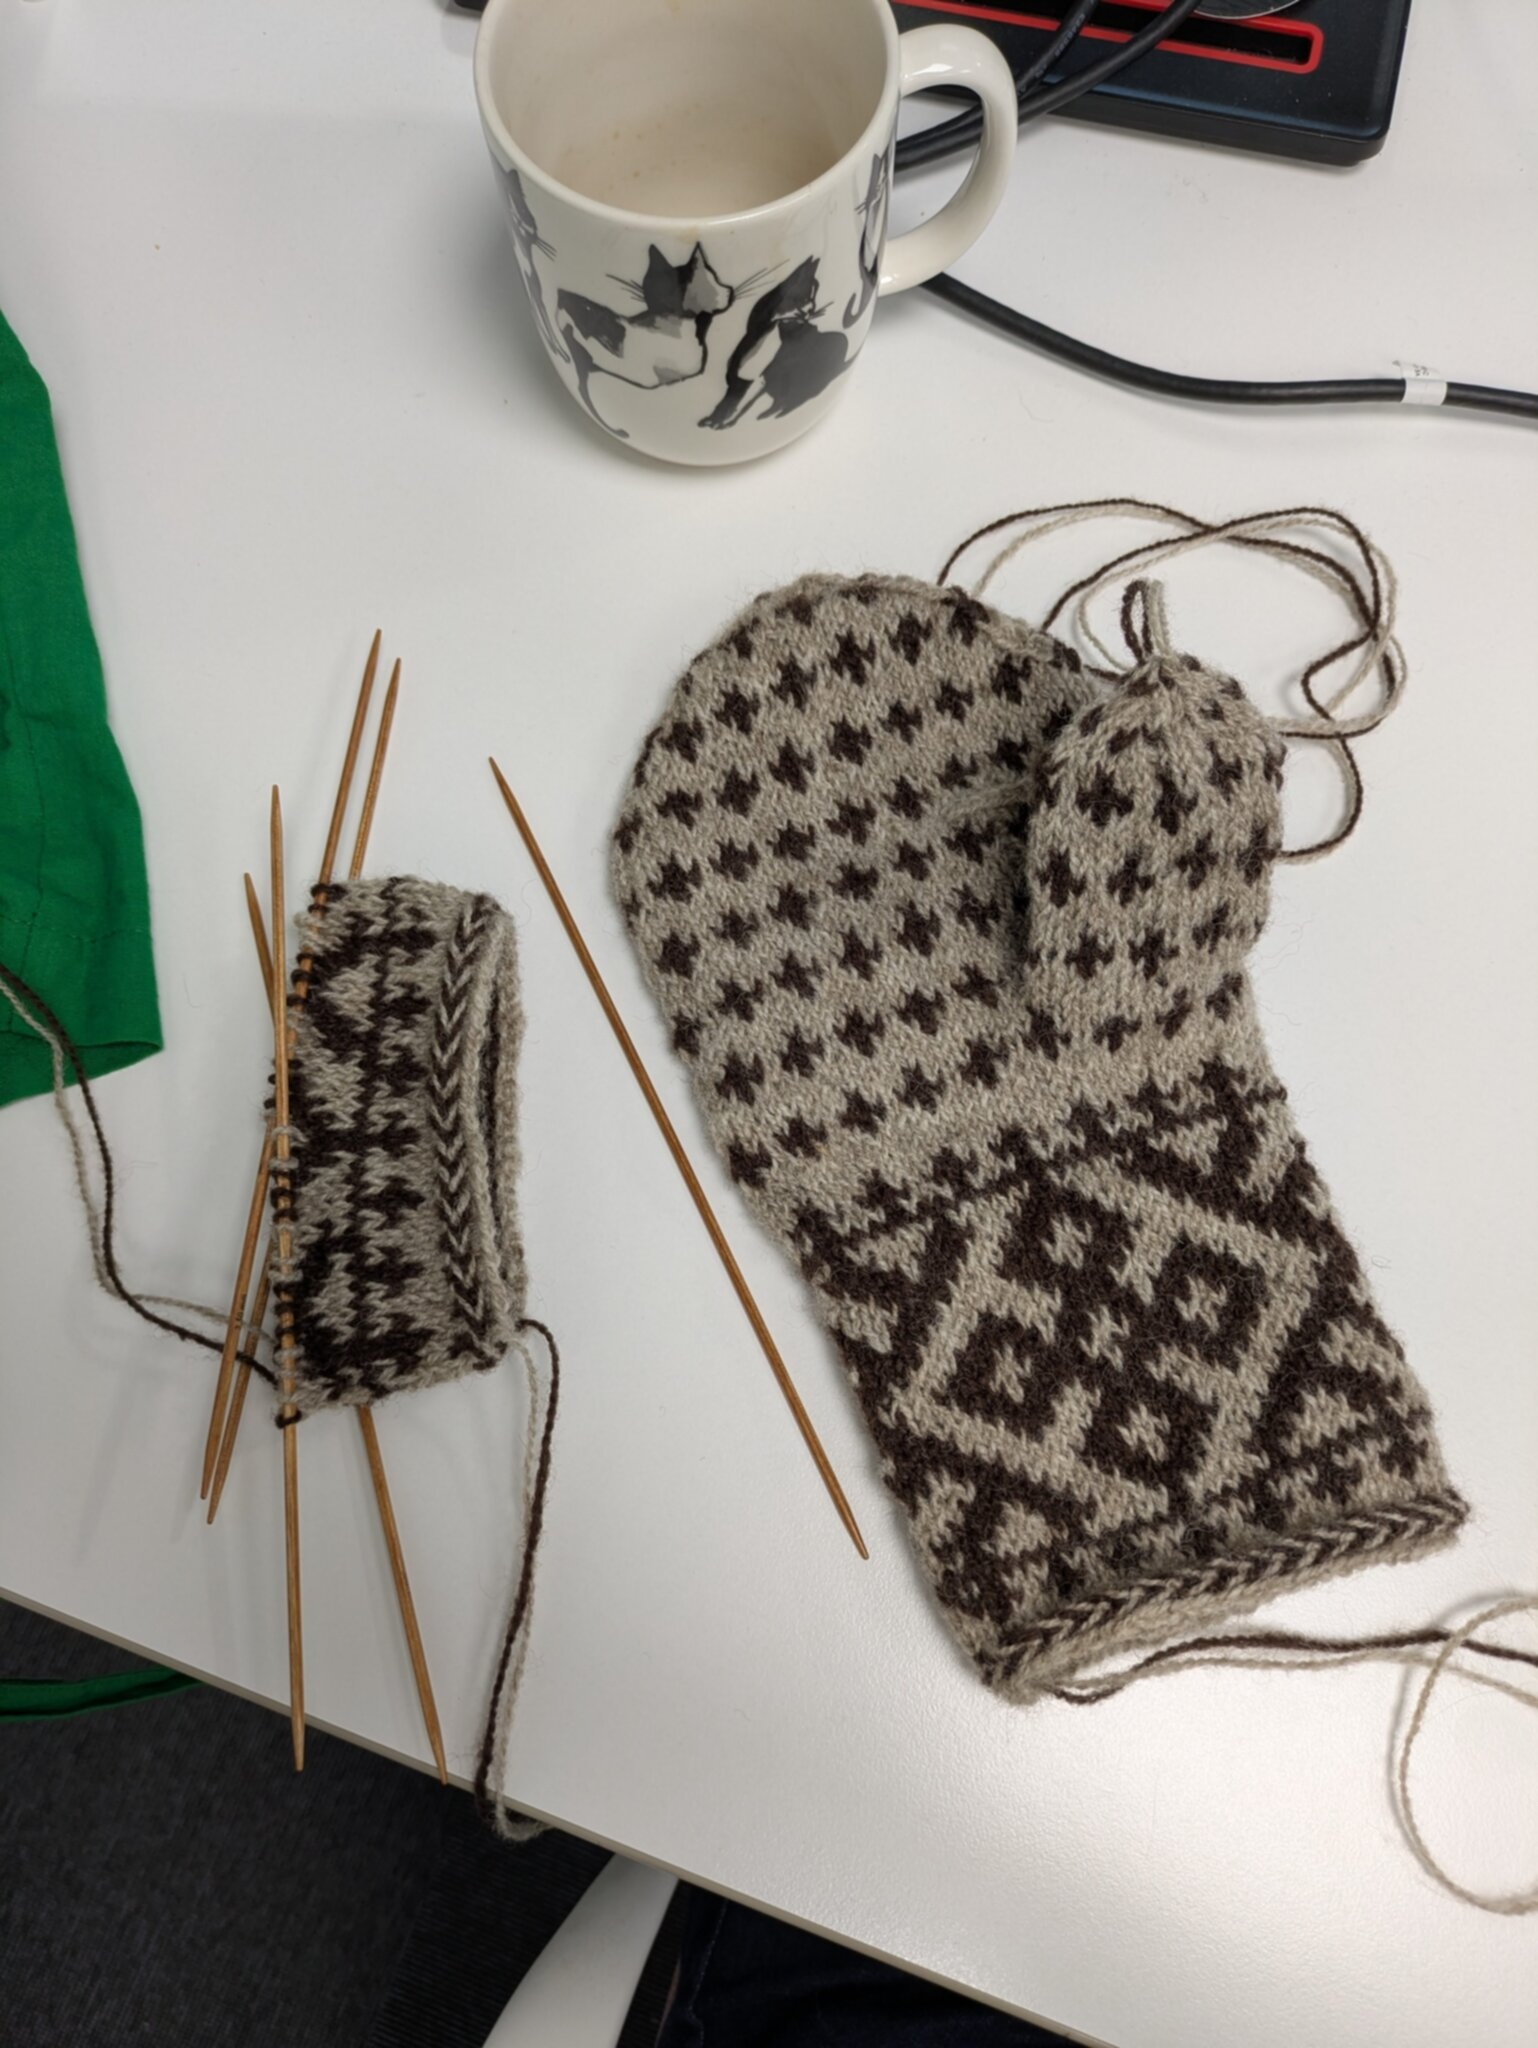
\includegraphics[width=0.9\linewidth]{assets/neulekilpailu1}
\end{wrapfigure}

Osallistumalla Tassun seuraavaan kilpailuun saatat ehkä olla \textbf{se},
joka suunnittelee KuRu:n seuraavan puolivirallisen vaatekappaleen. Me
ajattelimme, että olisi mukavaa saada KuRu:n oma neuleohje, jota kaikki
halukkaat jäsenet voisivat neuloa {\tiny(tai voisivat saada jonkun neulomaan
heille\ldots)} ja käyttää ylpeydellä.

Vaikka voi vaikuttaa siltä, että järjestämme kilpailun vain Anninalle,
\mbox{Nonnalle} ja Tanguylle, me haluamme, että se olisi mahdollisimman avoin
kaikille -- myös niille, joilla ei ole ollenkaan kokemusta neulesuunnittelusta
eikä neulomisesta. Täysin valmista neulepiirrosta ei tarvitse palauttaa eikä
\mbox{tarkkoja} silmukkalukuja ja kaikkea muuta. Jos sinulla on visio,
piirustuksia tai vain ideoita, kaikki käy, ja voidaan yhdessä valmistella
täydelliset ohjeet sen jälkeen, kun voittaja on valittu.

Vaatekappaleen tyyppi jätetään osallistujan päätettäväksi, mutta toivomme,
että se olisi sellainen, että useimmat voisivat toteuttaa sen olematta
konkareita, esimerkiksi lapaset, sukat, pipo, huivi tai vaikkapa kypärämyssy!

Arvostelemme ehdotukset kolmen kriteerin perusteella: Ehdotuksen kauneus (hyvin subjektiivista, kyllä kyllä), sen neulomisen helppous ja \mbox{''KuRu:maisuus''}.

Osallistu kilpailuun lähettämällä ehdotuksesi Tassun päätoimittajalle
sähköpostilla (osoitteen löydät lehden sisäkannesta) tai suoraan esimerkiksi
Whatsapp"-viestillä. Julkaisemme voittajan seuraavassa Tassussa.

\vfill

\begin{center}
	\noindent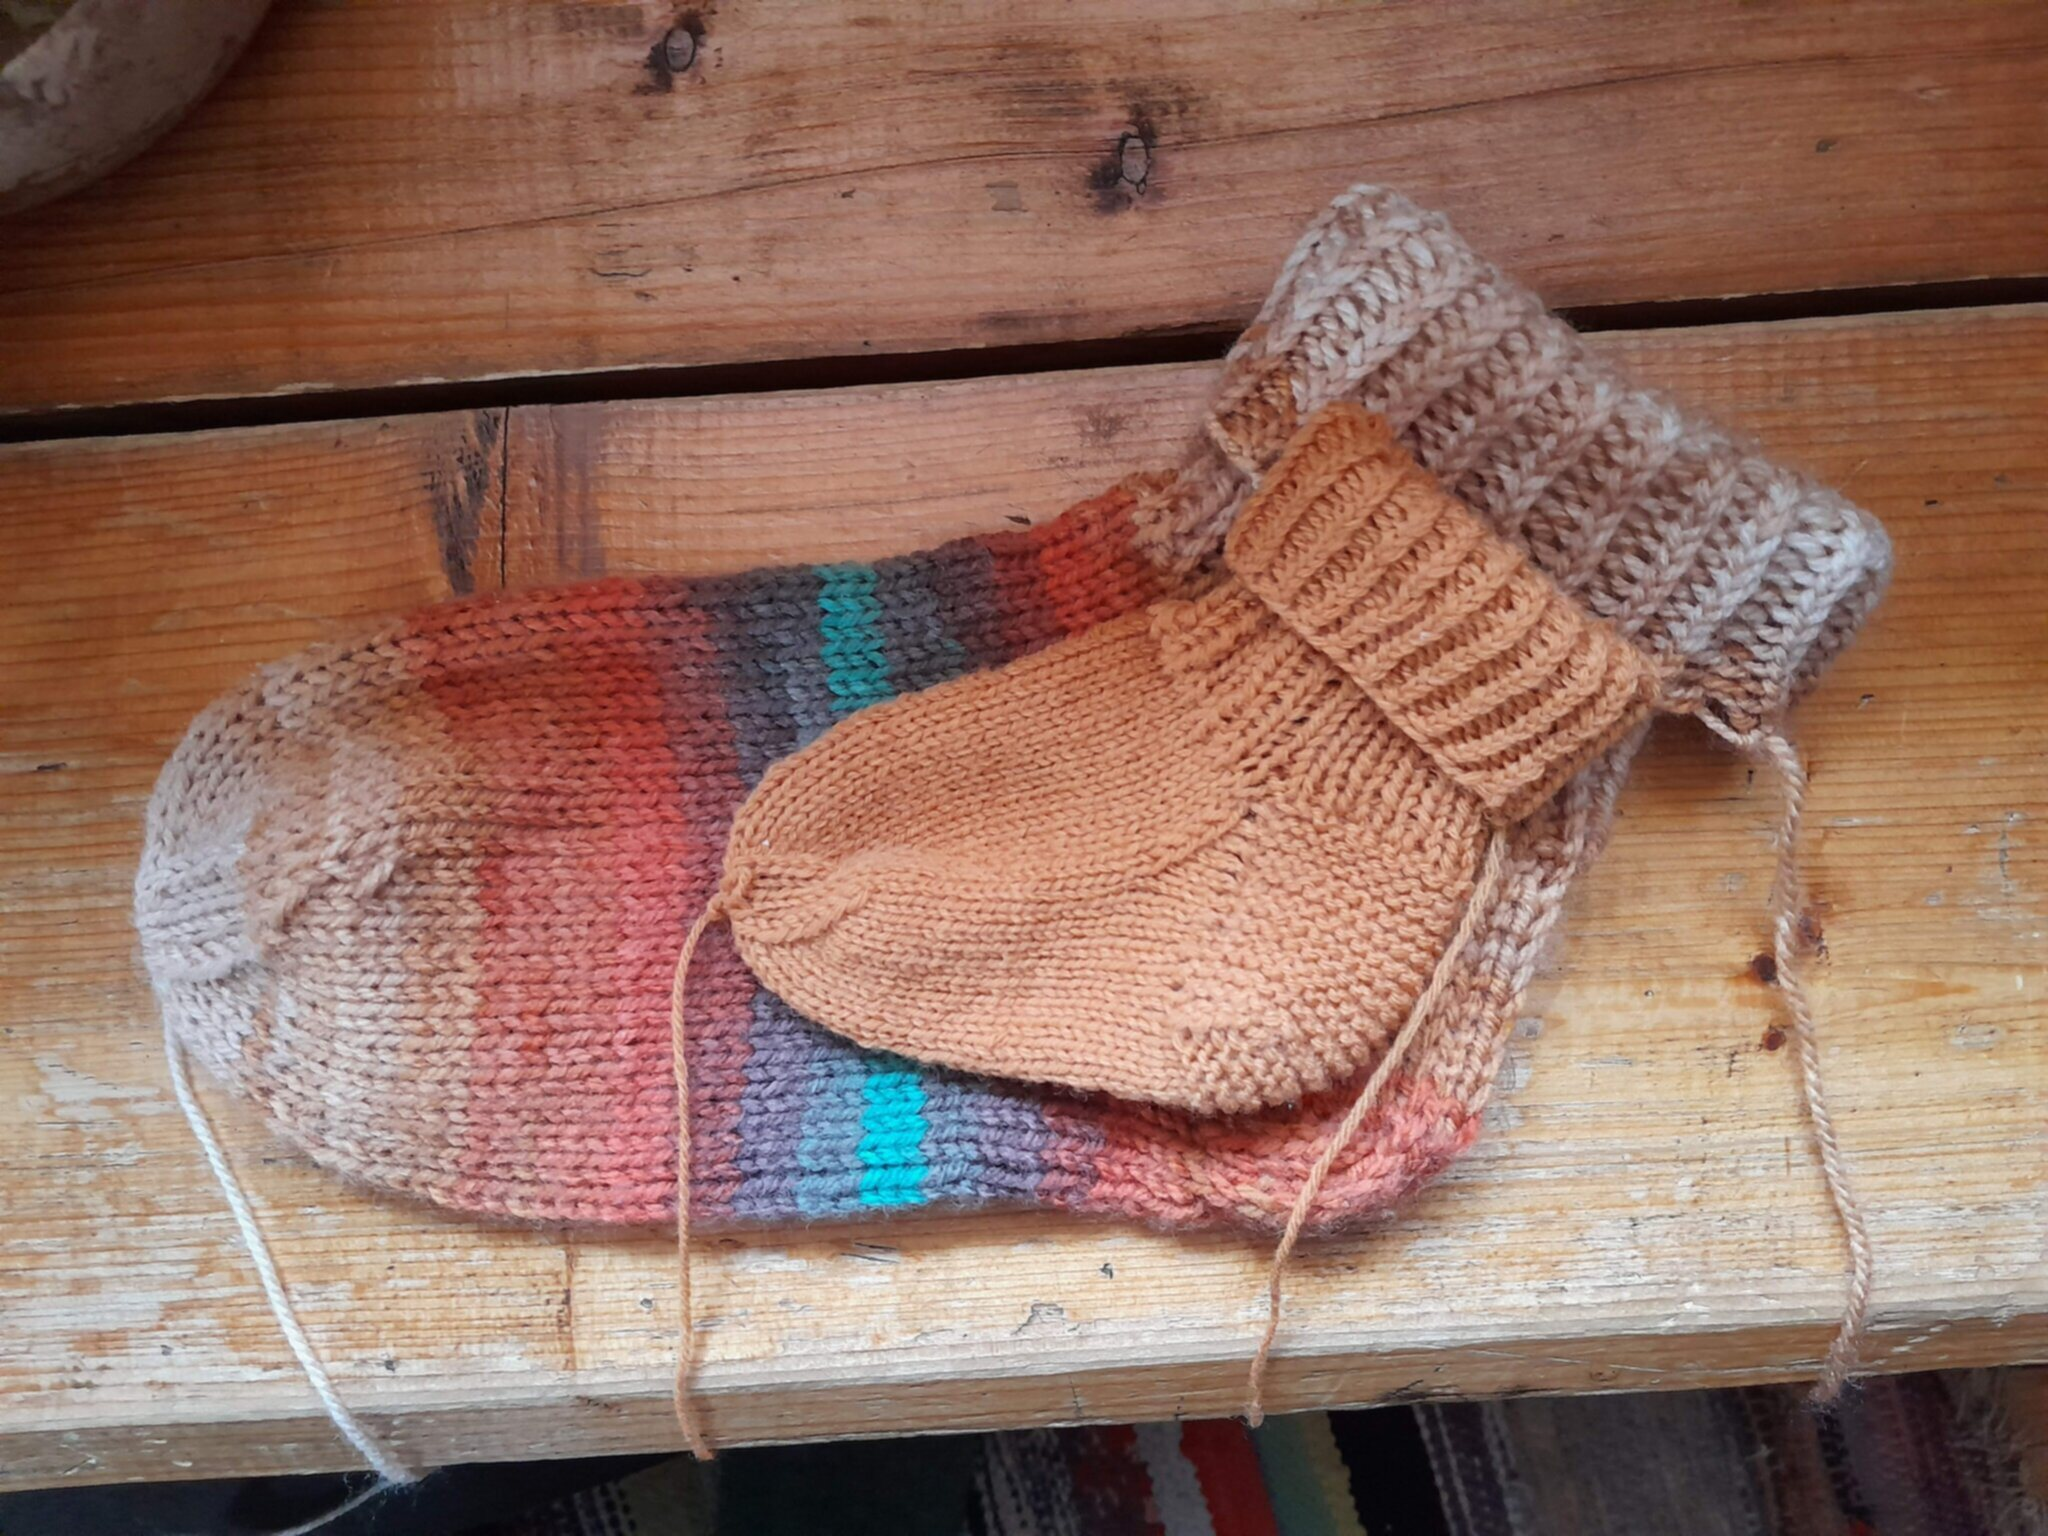
\includegraphics[width=0.8\linewidth,trim={0 9cm 0 9cm},clip]{assets/neulekilpailu2}
\end{center}


% \clearpage\section{Tulossa pian}

\clearpage

\thispagestyle{empty}
\newgeometry{left=2cm,right=1cm,top=1cm,bottom=1cm}
\ThisCenterWallPaper{1.07}{assets/no_auto_compression/takakansikuva.jpg}~

\vfill

\newtcolorbox{kuruboxendpage}[1][]{%
    enhanced,
    before skip=0mm,after skip=0mm, 
    width=0.68\textwidth, boxrule=0mm,
    colback=kuru, colframe=kuru, % Colors
    sharp corners,
    underlay={%
	    \fill[kuru] ([xshift=-8mm,yshift=3mm]frame.north west) -- ([yshift=1mm]frame.north east)
	    -- ([xshift=1mm,yshift=-3mm]frame.south east) -- ([xshift=-7mm,yshift=-1mm]frame.south west)
	    -- cycle;
	    \fill[white] ([xshift=-4mm,yshift=-1mm]frame.north west) ellipse (1mm and 2mm);
	    \fill[white] ([xshift=-1mm,yshift=-1mm]frame.north west) ellipse (1mm and 2mm);
	    \fill[white] ([xshift=-2.5mm,yshift=-5mm]frame.north west) circle (1mm);
	    \fill[white] ([xshift=-2.5mm,yshift=-8mm]frame.north west) circle (1mm);
        },
    % drop fuzzy shadow, % Shadow
    title={#1},
}

{
	\noindent
	\begin{addmargin}[0.32cm]{0cm}
		\begin{center}
			\begin{kuruboxendpage}[]
				\color{white}{\Large\bfseries 1/2025 Kurkisuon Rusakot ry}
			\end{kuruboxendpage}
		\end{center}
	\end{addmargin}
}


\end{document}
